%%%%%%%%%%%%%%%%%%%%%%%%%%%%%%%%%%%%%%%%%
% Masters/Doctoral Thesis 
% LaTeX Template
% Version 2.5 (27/8/17)
%
% This template was downloaded from:
% http://www.LaTeXTemplates.com
%
% Version 2.x major modifications by:
% Vel (vel@latextemplates.com)
%
% This template is based on a template by:
% Steve Gunn (http://users.ecs.soton.ac.uk/srg/softwaretools/document/templates/)
% Sunil Patel (http://www.sunilpatel.co.uk/thesis-template/)
%
% Template license:
% CC BY-NC-SA 3.0 (http://creativecommons.org/licenses/by-nc-sa/3.0/)
%
%%%%%%%%%%%%%%%%%%%%%%%%%%%%%%%%%%%%%%%%%

%----------------------------------------------------------------------------------------
%	PACKAGES AND OTHER DOCUMENT CONFIGURATIONS
%----------------------------------------------------------------------------------------

\documentclass[
11pt, % The default document font size, options: 10pt, 11pt, 12pt
%oneside, % Two side (alternating margins) for binding by default, uncomment to switch to one side
english, % ngerman for German
singlespacing, % Single line spacing, alternatives: onehalfspacing or doublespacing
%draft, % Uncomment to enable draft mode (no pictures, no links, overfull hboxes indicated)
%nolistspacing, % If the document is onehalfspacing or doublespacing, uncomment this to set spacing in lists to single
%liststotoc, % Uncomment to add the list of figures/tables/etc to the table of contents
%toctotoc, % Uncomment to add the main table of contents to the table of contents
parskip, % Uncomment to add space between paragraphs
%nohyperref, % Uncomment to not load the hyperref package
headsepline, % Uncomment to get a line under the header
%chapterinoneline, % Uncomment to place the chapter title next to the number on one line
%consistentlayout, % Uncomment to change the layout of the declaration, abstract and acknowledgements pages to match the default layout
]{MastersDoctoralThesis} % The class file specifying the document structure

\usepackage[utf8]{inputenc} % Required for inputting international characters
\usepackage[T1]{fontenc} % Output font encoding for international characters

\usepackage{mathpazo} % Use the Palatino font by default

\usepackage[sorting=none]{biblatex} % Use the bibtex backend with the authoryear citation style (which resembles APA)
% \usepackage[backend=bibtex,style=authoryear,natbib=true]{biblatex} % Use the bibtex backend with the authoryear citation style (which resembles APA)

% \addbibresource{example.bib} % The filename of the bibliography
\addbibresource{main.bib} % The filename of the bibliography

\usepackage[autostyle=true]{csquotes} % Required to generate language-dependent quotes in the bibliography

\usepackage{amsmath}  % Provides lots of good commands for math formulas.
\usepackage{subcaption}  % Provides the \subfigure command
\usepackage{epigraph}

%-----------------------------------------------------------------
% Code Formatting
\usepackage{listings}  % Provides pretty code formatting
\definecolor{codegray}{rgb}{0.5,0.5,0.5}
\definecolor{backgray}{rgb}{0.95,0.95,0.95}
\lstset{
	basicstyle=\footnotesize,
	% backgroundcolor=\color{backgray},
	% numberstyle=\color{codegray},
	xleftmargin=2em,
	numbers=left,
	numbersep=5pt,
	% frame=trBL,
	% frameround=fttt
}
% Better inline directory listings
\usepackage{xcolor}
\definecolor{light-gray}{gray}{0.95}
\newcommand{\code}[1]{\colorbox{light-gray}{\texttt{#1}}}

%----------------------------------------------------------------------------------------
%	MARGIN SETTINGS
%----------------------------------------------------------------------------------------

\geometry{
	paper=letterpaper, % Change to letterpaper for US letter
	inner=2.5cm, % Inner margin
	outer=3.8cm, % Outer margin
	bindingoffset=.5cm, % Binding offset
	top=1.5cm, % Top margin
	bottom=1.5cm, % Bottom margin
	%showframe, % Uncomment to show how the type block is set on the page
}

%----------------------------------------------------------------------------------------
%	THESIS INFORMATION
%----------------------------------------------------------------------------------------

\thesistitle{DIY Supercube} % Your thesis title, this is used in the title and abstract, print it elsewhere with \ttitle
\supervisor{Dr. Robert \textsc{Heinrichs}} % Your supervisor's name, this is used in the title page, print it elsewhere with \supname
\examiner{} % Your examiner's name, this is not currently used anywhere in the template, print it elsewhere with \examname
\degree{Honors Thesis in Software Engineering} % Your degree name, this is used in the title page and abstract, print it elsewhere with \degreename
\author{Joseph \textsc{Hale}} % Your name, this is used in the title page and abstract, print it elsewhere with \authorname
\addresses{} % Your address, this is not currently used anywhere in the template, print it elsewhere with \addressname

\subject{Software Engineering} % Your subject area, this is not currently used anywhere in the template, print it elsewhere with \subjectname
\keywords{} % Keywords for your thesis, this is not currently used anywhere in the template, print it elsewhere with \keywordnames
\university{\href{http://www.asu.edu}{Arizona State University}} % Your university's name and URL, this is used in the title page and abstract, print it elsewhere with \univname
\department{\href{http://department.university.com}{Barrett, The Honors College}} % Your department's name and URL, this is used in the title page and abstract, print it elsewhere with \deptname
\group{\href{http://researchgroup.university.com}{Fulton Schools of Engineering}} % Your research group's name and URL, this is used in the title page, print it elsewhere with \groupname
\faculty{\href{http://faculty.university.com}{Dr. Robert Heinrichs}} % Your faculty's name and URL, this is used in the title page and abstract, print it elsewhere with \facname

\AtBeginDocument{
	\hypersetup{pdftitle=\ttitle} % Set the PDF's title to your title
	\hypersetup{pdfauthor=\authorname} % Set the PDF's author to your name
	\hypersetup{pdfkeywords=\keywordnames} % Set the PDF's keywords to your keywords
	
	% Set colors of the various links within the PDF document.
	% A good summary can be found here: https://tex.stackexchange.com/a/50754
	\hypersetup{colorlinks=true} % Don't color links in the print version
	\hypersetup{urlcolor=[rgb]{0.2549,0.0353,0.3569}} % Set the color of hyperlinks to ProblemSolved-You's Purple
	\hypersetup{linkcolor=[rgb]{0.2549,0.0353,0.3569}} % Set the color of hyperlinks to  ProblemSolved-You's Purple
	\hypersetup{citecolor=[rgb]{0.2549,0.0353,0.3569}} % Set the color of hyperlinks to ProblemSolved-You's Purple
}

\begin{document}

\frontmatter % Use roman page numbering style (i, ii, iii, iv...) for the pre-content pages

\pagestyle{plain} % Default to the plain heading style until the thesis style is called for the body content

%----------------------------------------------------------------------------------------
%	TITLE PAGE
%----------------------------------------------------------------------------------------

\begin{titlepage}
\begin{center}

\vspace*{.06\textheight}
{\scshape\LARGE \univname\par}\vspace{1.5cm} % University name
\textsc{\Large Honors Thesis}\\[0.5cm] % Thesis type

\HRule \\[0.4cm] % Horizontal line
{\huge \bfseries \ttitle\par}\vspace{0.4cm} % Thesis title
\HRule \\[1.5cm] % Horizontal line
 
\begin{minipage}[t]{0.4\textwidth}
\begin{flushleft} \large
\emph{Author:}\\
\href{https://github.com/jhale1805}{\authorname} % Author name - remove the \href bracket to remove the link
\end{flushleft}
\end{minipage}
\begin{minipage}[t]{0.4\textwidth}
\begin{flushright} \large
\emph{Supervisor:} \\
\href{https://isearch.asu.edu/profile/3180015}{\supname} % Supervisor name - remove the \href bracket to remove the link  
\end{flushright}
\end{minipage}\\[3cm]
 
\vfill

\large \textit{A thesis submitted in fulfillment of the requirements\\ for the degree of \degreename}\\[0.3cm] % University requirement text
\textit{in the}\\[0.4cm]
\groupname\\\deptname\\[2cm] % Research group name and department name
 
\vfill

{\large \today}\\[4cm] % Date
%\includegraphics{Logo} % University/department logo - uncomment to place it
 
\vfill
\end{center}
\end{titlepage}

%----------------------------------------------------------------------------------------
%	DECLARATION PAGE
%----------------------------------------------------------------------------------------

\begin{declaration}
\addchaptertocentry{\authorshipname} % Add the declaration to the table of contents
\noindent I, \authorname, declare that this thesis titled, \enquote{\ttitle} and the work presented in it are my own. I confirm that:

\begin{itemize} 
\item This work was done wholly or mainly while in candidature for a research degree at this University.
\item Where any part of this thesis has previously been submitted for a degree or any other qualification at this University or any other institution, this has been clearly stated.
\item Where I have consulted the published work of others, this is always clearly attributed.
\item Where I have quoted from the work of others, the source is always given. With the exception of such quotations, this thesis is entirely my own work.
\item I have acknowledged all main sources of help.
\item Where the thesis is based on work done by myself jointly with others, I have made clear exactly what was done by others and what I have contributed myself.\\
\end{itemize}
 
\noindent Signed:\\
\rule[0.5em]{25em}{0.5pt} % This prints a line for the signature
 
\noindent Date:\\
\rule[0.5em]{25em}{0.5pt} % This prints a line to write the date
\end{declaration}

\cleardoublepage

%----------------------------------------------------------------------------------------
%	QUOTATION PAGE
%----------------------------------------------------------------------------------------

\vspace*{0.2\textheight}

\noindent\enquote{\itshape Thanks to my solid academic training, today I can write hundreds of words on virtually any topic without possessing a shred of information, which is how I got a good job in journalism.}\bigbreak

\hfill Dave Barry

%----------------------------------------------------------------------------------------
%	ABSTRACT PAGE
%----------------------------------------------------------------------------------------

\begin{abstract}
\addchaptertocentry{\abstractname} % Add the abstract to the table of contents
The Thesis Abstract is written here (and usually kept to just this page). The page is kept centered vertically so can expand into the blank space above the title too\ldots
\end{abstract}

%----------------------------------------------------------------------------------------
%	ACKNOWLEDGEMENTS
%----------------------------------------------------------------------------------------

\begin{acknowledgements}
\addchaptertocentry{\acknowledgementname} % Add the acknowledgements to the table of contents
The acknowledgments and the people to thank go here, don't forget to include your project advisor\ldots
\end{acknowledgements}

%----------------------------------------------------------------------------------------
%	LIST OF CONTENTS/FIGURES/TABLES PAGES
%----------------------------------------------------------------------------------------

\tableofcontents % Prints the main table of contents

\listoffigures % Prints the list of figures

\listoftables % Prints the list of tables

%----------------------------------------------------------------------------------------
%	ABBREVIATIONS
%----------------------------------------------------------------------------------------

\begin{abbreviations}{ll} % Include a list of abbreviations (a table of two columns)

\textbf{PCB} & \textbf{P}rinted \textbf{C}ircuit \textbf{B}oard\\
\textbf{TPS} & \textbf{T}urns \textbf{P}er \textbf{S}econd\\
\textbf{WCA} & \textbf{W}orld \textbf{C}ube \textbf{A}ssociation\\

\end{abbreviations}

%----------------------------------------------------------------------------------------
%	PHYSICAL CONSTANTS/OTHER DEFINITIONS
%----------------------------------------------------------------------------------------

\begin{constants}{lr@{${}={}$}l} % The list of physical constants is a three column table

% The \SI{}{} command is provided by the siunitx package, see its documentation for instructions on how to use it

Speed of Light & $c_{0}$ & \SI{2.99792458e8}{\meter\per\second} (exact)\\
%Constant Name & $Symbol$ & $Constant Value$ with units\\

\end{constants}

%----------------------------------------------------------------------------------------
%	SYMBOLS
%----------------------------------------------------------------------------------------

\begin{symbols}{lll} % Include a list of Symbols (a three column table)

$a$ & distance & \si{\meter} \\
$P$ & power & \si{\watt} (\si{\joule\per\second}) \\
%Symbol & Name & Unit \\

\addlinespace % Gap to separate the Roman symbols from the Greek

$\omega$ & angular frequency & \si{\radian} \\

\end{symbols}

%----------------------------------------------------------------------------------------
%	DEDICATION
%----------------------------------------------------------------------------------------

\dedicatory{For/Dedicated to/To my\ldots} 

%----------------------------------------------------------------------------------------
%	THESIS CONTENT - CHAPTERS
%----------------------------------------------------------------------------------------

\mainmatter % Begin numeric (1,2,3...) page numbering

\pagestyle{thesis} % Return the page headers back to the "thesis" style

% Include the chapters of the thesis as separate files from the Chapters folder
% Uncomment the lines as you write the chapters

% Chapter Template

\chapter{Introduction} % Main chapter title

\label{Chapter1} % Change X to a consecutive number; for referencing this chapter elsewhere, use \ref{ChapterX}

% TODO What are we looking at? What will be shown? State general research questions to answer. Start by defining the *problem*. The rest of the thesis will detail my solution.

% I am trying to persuade someone that a sound-based smart cube is viable on consumer grade hardware.

\section{The Advent of Smart Cubes}
Speedsolving, the sport of solving twisty puzzles like the Rubik’s Cube as fast as possible, has seen a resurgence of popularity since the early 2000s. % TODO add citation 
Over the past two decades many advances in cube technology have produced ever higher performing puzzles. 

Recently, the speedcubing community has seen the entrance of smart cubes, special versions of a Rubik’s Cube that can connect to a mobile device over Bluetooth. 
These smart cubes have sparked a wave of excitement with the vast opportunities they offer for automatic turn tracking, performance analysis, personalized improvement feedback, and networked competition.

\section{Obstacles to Adoption}
While a revolutionary idea, smart cubes still face several obstacles to widespread adoption. 

\begin{itemize}
    \item \emph{Cost}: Smart cubes can cost up to eight times as much as a comparable non-smart speedcube. For example, one popular budget speedcube, the Moyu Weilong, costs only \$5, while the cheapest smartcube, the Giiker Cube, starts at \$40. [TODO sources!]. On the higher end, a premium speedcube, like the Gans 356 XS, retails for just over \$60 while a premium smartcube, like the GoCube, retails for over \$100. [TODO Make this a footnote.]
    \item \emph{Performance}: Existing smart cubes turn slower than comparable non-smart cubes. [TODO source]
    \item \emph{Reliability}: Many smart cube owners report inability to connect the smart cube to a mobile device and missed/inaccurate turn tracking.
    \item \emph{Regulation}: Current competition rules ban the use of electronics during timed solves, thus banning the use of smart cubes. There is no foreseeable change to this rule. 
\end{itemize}

As a result of these obstacles, many speedcubers refrain from purchasing a smart cube, despite expressing significant interest in the opportunities smart cubes offer.

\section{Purpose of this Thesis}
The primary goal of this thesis is to create a proof-of-concept for a smart cube design that mitigates the performance and competitive regulatory concerns of existing smartcubes.

\subsection{Design Requirements}
TODO 

Specifically, the smart cube design discussed in this thesis will be assessed against the following criteria:
\begin{enumerate}
    \item \emph{Compatibility with Standard Speedcubes}: The design must be deployable within a standard (non-smart) speedcube. "How can a standard speedcube be enhanced into a smart cube?"
        \begin{enumerate} 
            \item The design must not require permanent modifications to the original speedcube.
            \item The design must not significantly impact the turn-speed of the original speedcube.
        \end{enumerate}
    \item \emph{Move Tracking Accuracy}: The design must be capable of tracking the face turns of a Rubik's Cube with over 99\% accuracy. 
    \item \emph{Move Tracking Granularity}: The design must be capable of recording the time spent executing each individual face turn of a Rubik's Cube.
    \item \emph{Competition Legality}: The design must be competition legal, meaning it results in a cube that either does not violate existing competition rules against the use of electronics or can be easily modified to regain compliance.
\end{enumerate}

\section{Thesis Overview}
TODO give an overview of the rest of the Thesis document.
% Chapter Template

\chapter{Background} % Main chapter title

\label{Chapter2} % Change X to a consecutive number; for referencing this chapter elsewhere, use \ref{ChapterX}


\section{A Brief History of the Rubik's Cube}

In 1974, Erno Rubik, a Hungarian professor of architecture, sought to help his students visualize space in three dimensions. To that end, he created a special cube whose faces could independently rotate around all three physical axes \cite{rubik-motivation}. When he added colored stickers to further aid in visualizing the movements, Mr. Rubik realized he had created a new puzzle. He patented his cube in 1975, \cite{rubik-patent} and since then over 450 million units have been sold \cite{forbes-rubik-merger}, allowing an estimated 1 in 7 humans on earth to try their hand at solving it \cite{rubik-population-reached}.

Since then, the cube has been the subject of academic research, competition, leisure, and cultural iconography.


\section{Rubik's Cube Mechanics}

Nunc posuere quam at lectus tristique eu ultrices augue venenatis. Vestibulum ante ipsum primis in faucibus orci luctus et ultrices posuere cubilia Curae; Aliquam erat volutpat. Vivamus sodales tortor eget quam adipiscing in vulputate ante ullamcorper. Sed eros ante, lacinia et sollicitudin et, aliquam sit amet augue. In hac habitasse platea dictumst.

\subsection{Subsection 1}
Nunc posuere quam at lectus tristique eu ultrices augue venenatis. Vestibulum ante ipsum primis in faucibus orci luctus et ultrices posuere cubilia Curae; Aliquam erat volutpat. Vivamus sodales tortor eget quam adipiscing in vulputate ante ullamcorper. Sed eros ante, lacinia et sollicitudin et, aliquam sit amet augue. In hac habitasse platea dictumst.

\subsection{Subsection 2}
Morbi rutrum odio eget arcu adipiscing sodales. Aenean et purus a est pulvinar pellentesque. Cras in elit neque, quis varius elit. Phasellus fringilla, nibh eu tempus venenatis, dolor elit posuere quam, quis adipiscing urna leo nec orci. Sed nec nulla auctor odio aliquet consequat. Ut nec nulla in ante ullamcorper aliquam at sed dolor. Phasellus fermentum magna in augue gravida cursus. Cras sed pretium lorem. Pellentesque eget ornare odio. Proin accumsan, massa viverra cursus pharetra, ipsum nisi lobortis velit, a malesuada dolor lorem eu neque.


\section{The World Cube Association}

Sed ullamcorper quam eu nisl interdum at interdum enim egestas. Aliquam placerat justo sed lectus lobortis ut porta nisl porttitor. Vestibulum mi dolor, lacinia molestie gravida at, tempus vitae ligula. Donec eget quam sapien, in viverra eros. Donec pellentesque justo a massa fringilla non vestibulum metus vestibulum. Vestibulum in orci quis felis tempor lacinia. Vivamus ornare ultrices facilisis. Ut hendrerit volutpat vulputate. Morbi condimentum venenatis augue, id porta ipsum vulputate in. Curabitur luctus tempus justo. Vestibulum risus lectus, adipiscing nec condimentum quis, condimentum nec nisl. Aliquam dictum sagittis velit sed iaculis. Morbi tristique augue sit amet nulla pulvinar id facilisis ligula mollis. Nam elit libero, tincidunt ut aliquam at, molestie in quam. Aenean rhoncus vehicula hendrerit.

\subsection{Competition Regulations}
Nunc posuere quam at lectus tristique eu ultrices augue venenatis. Vestibulum ante ipsum primis in faucibus orci luctus et ultrices posuere cubilia Curae; Aliquam erat volutpat. Vivamus sodales tortor eget quam adipiscing in vulputate ante ullamcorper. Sed eros ante, lacinia et sollicitudin et, aliquam sit amet augue. In hac habitasse platea dictumst. 
% Chapter Template

\chapter{State of the Art} % Main chapter title

\label{Chapter3} % Change X to a consecutive number; for referencing this chapter elsewhere, use \ref{ChapterX}


\section{Introduction}

TODO, be a *neutral* presentation of the current state of this technology. Give a big information dump to the reader.


\section{Commercial Smartcubes}

Commercial Smartcubes are special Rubik's Cubes built around sensors that can detect face turns and transmit that information over Bluetooth.
Some models can also measure and transmit data about the cube's orientation.

At the time of writing, there are three major smartcubes on the market: the Giiker Cube, the Go Cube, and the Gans 356i.
This section will discuss the internal components of each of these cubes that provide this move-tracking functionality.

\subsection{Giiker Cube}
The Xiaomi Giiker Cube was released in September 2018 making it the first commercial smartcube on the market \cite{giiker-thecubicle}.
This "Supercube" as it was branded, used a relatively simple system for tracking the cube's movements.
The core of the cube is built around a small circuit board with a microcontroller that measures the cube's movements and a bluetooth antenna that transmits those moves wirelessly (Figure ~\ref{fig:giiker-internal-board}).
The microcontroller detects each face turn by reading the voltage drop across a small circuit embedded within each center cap (Figure ~\ref{fig:giiker-center-front}).
The center cap circuit controls its output voltage by using a copper brush to change between four separate electric paths, three different resistors and ground, as each face rotates (Figure ~\ref{fig:giiker-center-brush}). \cite{giiker-internals}


% How to do a sub-figure: https://tex.stackexchange.com/a/37597
\begin{figure}
    \centering
    \begin{subfigure}{0.25\textwidth}
        \centering
        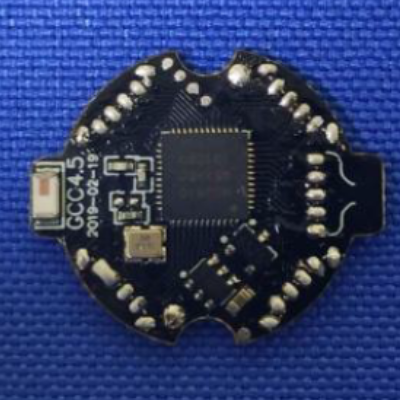
\includegraphics[width=.90\linewidth]{Figures/3 State of the Art/giiker-internal-board.png}
        \caption{Internal Board \cite{giiker-internals}}
        \label{fig:giiker-internal-board}
    \end{subfigure}%
    \begin{subfigure}{0.25\textwidth}
        \centering
        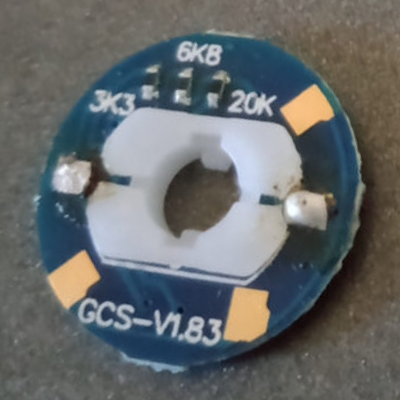
\includegraphics[width=.90\linewidth]{Figures/3 State of the Art/giiker-center-front.png}
        \caption{Center Cap Board \cite{eggins-giiker-internals}}
        \label{fig:giiker-center-front}
    \end{subfigure}%
    \begin{subfigure}{0.25\textwidth}
        \centering
        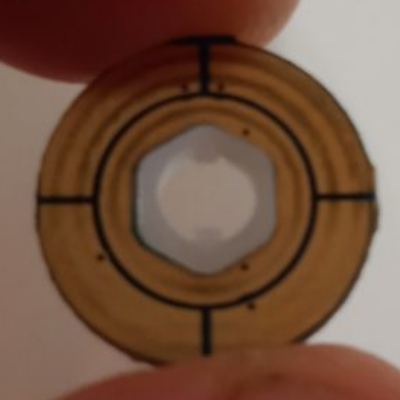
\includegraphics[width=.90\linewidth]{Figures/3 State of the Art/giiker-center-pads.png}
        \caption{Center Cap Pads \cite{eggins-giiker-internals}}
        \label{fig:giiker-center-pads}
    \end{subfigure}%
    \begin{subfigure}{0.25\textwidth}
        \centering
        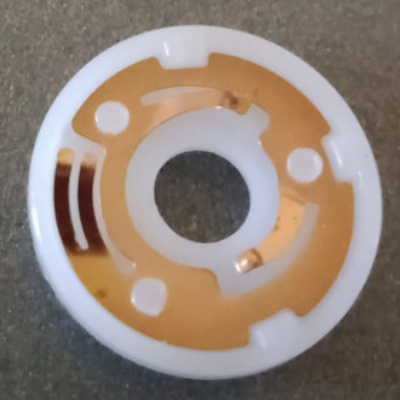
\includegraphics[width=.90\linewidth]{Figures/3 State of the Art/giiker-center-brush.png}
        \caption{Center Cap Brush \cite{eggins-giiker-internals}}
        \label{fig:giiker-center-brush}
    \end{subfigure}%
    \caption{The internal components of the Giiker Cube}
    \label{fig:giiker-internal-components}
\end{figure}

\subsection{Go Cube}
Announced on Kickstarter in June 2018, Patricula's GoCube was the first smartcube to include a gyroscope that would track a Rubik's Cube's orientation in addition to the face turns applied to it. \cite{gocube-product-launch-video}
Like the Giiker Cube before it, the GoCube's core contains a small circuit board with the main electronics including a microcontroller, bluetooth antenna, and the added gyroscope (Figure ~\ref{fig:gocube-core}). 
Though the teardown pictures from the Go Cube's FCC filing aren't particularly clear, it appears that the cube produces a voltage drop by changing which one of the four resistors across the bottom of the center cap board is in series with the circuit (Figure ~\ref{fig:gocube-cap-chip})

% How to do a sub-figure: https://tex.stackexchange.com/a/37597
\begin{figure}
    \centering
    \begin{subfigure}{0.25\textwidth}
        \centering
        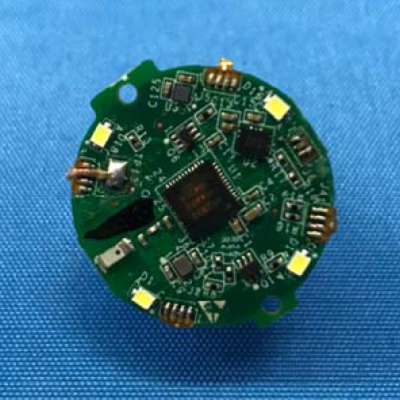
\includegraphics[width=.90\linewidth]{Figures/3 State of the Art/gocube-core.png}
        \caption{Internal Board}
        \label{fig:gocube-core}
    \end{subfigure}%
    \begin{subfigure}{0.25\textwidth}
        \centering
        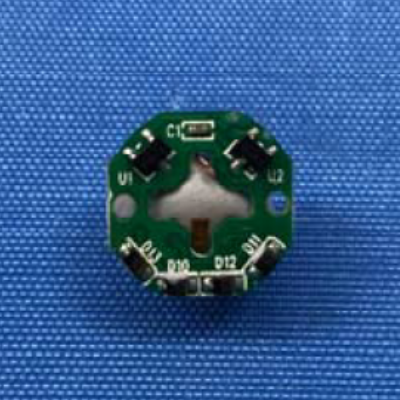
\includegraphics[width=.90\linewidth]{Figures/3 State of the Art/gocube-cap-chip.png}
        \caption{Center Cap Board}
        \label{fig:gocube-cap-chip}
    \end{subfigure}%
    \begin{subfigure}{0.50\textwidth}
        \centering
        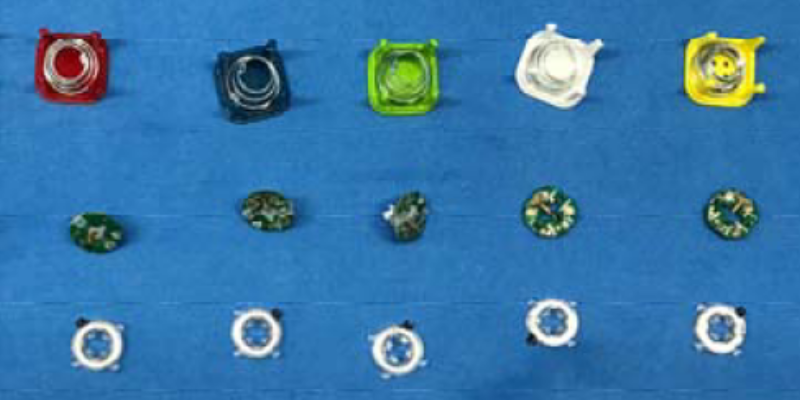
\includegraphics[width=.90\linewidth]{Figures/3 State of the Art/gocube-centers.png}
        \caption{Full Center Cap Teardown}
        \label{fig:gocube-centers}
    \end{subfigure}%
    \caption{The internal components of the Go Cube \cite{gocube-internals}
    \cite{gocube-internals}
    \cite{gocube-internals}}
    \label{fig:gocube-internal-components}
\end{figure}

\subsection{Gans 356i}
Released in July 2019, the Gans 356i was the first commercial smartcube produced by a traditional speedcube manufacturer. \cite{gans356i-thecubicle}
While the Gans 356i also uses a microcontroller to process the face turns and Bluetooth to transmit the move data, it tracks moves not through changing resistors in and out of a circuit, but via six plastic rods that connect the outer center caps to internal rotary encoders (Figure ~\ref{fig:gans356i-core}).

\begin{figure}
    \centering
    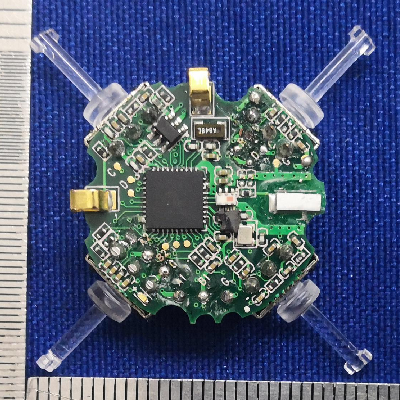
\includegraphics{Figures/3 State of the Art/gans356i-core.png}
    \decoRule
    \caption[Gans 356i Teardown]{The Gans 356i Cube's internal components. \cite{gans-356i-internals}}
    \label{fig:gans356i-core}
\end{figure}


\section{Academia}

\subsection{Rotary Encoders + Bluetooth}
TODO Discuss the viability of using rotary encoders + bluetooth for making a smart cube. Make sure to discuss the difference between absolute/relative rotary encoders.


\subsection{Sound}
TODO discuss the viability of using sound for making a smart cube.

\subsubsection{Google's "Data Over Sound" Project}
TODO discuss the Google's "data over sound" project and its applicability to this problem space.


\subsection{Computer Vision}
Computer Vision refers to the "field of Artificial Intelligence (AI) that enables computers and systems to derive meaningful information from digital images, videos, and other visual inputs." \cite{ibm-cv-definition}
Since human manipulation of a Rubik's Cube is a physical, observable process, Computer Vision algorithms could be developed to extract face turn information from videos of Rubik's Cube solutions.

This section summarizes some of the relevant research in this area, including computer vision algorithms capable of extracting individual sticker colors from video, measuring the angle of rotation of a specific face, and detection of entire face turns and face turn sequences.

\subsubsection{Sticker Color Classification}
In 2015, Jay Hack, an graduate student studying Computer Science at Stanford developed a neural network capable of recognizing the colors of a Rubik's Cube face from video in various lighting conditions.
His algorithm could classify frames within 7 milliseconds with 92\% accuracy. \cite{hackrubik}

\subsubsection{Measuring a Face's Angle of Rotation}
In 2019, OpenAI et al. published a viral video of a robot hand that had taught itself to solve a Rubik's Cube.
While the final, most successful version of the robot hand's software used a Giiker Cube to obtain the current rotational state of the cube, OpenAI et al. also researched the viability of tracking a Rubik's Cube's position using only computer vision.
Their most successful vision-only algorithm measured only the rotation angle of the top-most face on the Rubik's Cube and assumed significant hardware requirements: a modified sticker set for the Rubik's Cube, a well-lit environment, three strategically positioned RBG Basler cameras, and a neural network trained on "a pool of optimizer nodes, each of which uses 8 NVIDIA V100 GPUs and 64 CPU cores".
At peak performance, their vision-only algorithm's average error (the difference between the predicted face angle and the actual face angle) was 15.92$^\circ$, nearly three times the 5.90$^\circ$ average error of the hardware-based face angle measurement. \cite{openai2019rubiks}

\subsubsection{Classification of Single Moves and Entire Move Sequences}
In 2020, Junshen Kevin Chen, Wanze Xie, and Zhouheng Sun, graduate Computer Science students at Stanford created the DeepCube dataset consisting of over 20,000 videos of Rubik's Cube face turns with consistent lighting and backgrounds. 
They also built a neural network to classify the videos with the face turn they contained.
Their best performing model only made "one mistake every 15 moves" which corresponds to a 93.3\% accuracy. \cite{chendeepcube}


\subsection{Other Approaches}

TODO In this section I'm laying out a structure for discussing several of the options I looked into but ultimately disregarded. Should that go in the State of the Art chapter? or would it fit better in the Evaluation chapter to contrast against the potential of the sound-based implementation?

\subsubsection{RFID}
TODO discuss the viability of using RFID for making a smart cube.
\subsubsection{Magnetic Resonance}
TODO discuss the viability of using magnetic resonance for making a smart cube.
\subsubsection{Muscle-Tracking Armband}
TODO discuss the viability of using a muscle tracking armband for making a smart cube.


\section{Choice of Sound for My Thesis}

TODO This section might be large enough to merit its own chapter...
TODO Briefly detail the rationale for chosing to pursue a sound-based approach.
% Chapter Template

\chapter{Protocol Design} % Main chapter title

\label{Chapter4} % Change X to a consecutive number; for referencing this chapter elsewhere, use \ref{ChapterX}

\section{Introduction}
Designing a sound-based protocol for tracking the moves of a Rubik's Cube requires great care.
Lots of things produce sound that could interfere with the protocol: people talking, machines operating, nature stirring, and so forth.
Furthermore, the structure of the Rubik's Cube itself imposes stringent physical constraints on the size of any components used to produce the sounds used in the protocol.

This chapter first seeks to clearly detail the specific constraints that must be considered when designing a sound-based protocol for tracking the moves of a Rubik's Cube (\ref{sec:requirements}).
From there, a specific protocol will be proposed in Section \ref{sec:specification} for use in the successive chapters of this thesis.
This proposed protocol will be contrasted with an alternative option in Section \ref{sec:alternatives}.


\section{Requirements}
\label{sec:requirements}
This section will detail the constraints required for designing a protocol for tracking the moves of a Rubik's Cube.

These constraints include a sufficiently strong signal-to-noise ratio (\ref{subsec:signal-to-noise-ratio}), sufficient distinctiveness between tones (\ref{subsec:tone-distinctiveness}), the frequency response range of consumer hardware (\ref{subsec:frequency-response-range}), and the human auditory range (\ref{subsec:human-auditory-range}).

\subsection{Signal-to-Noise Ratio}
\label{subsec:signal-to-noise-ratio}
Sound is an easily accessible, and therefore noisy, medium of communication.
As a result, any data transmission protocol based on sound must be resilient to the presence of additional noise unrelated to the signal being transmitted.
For a sound-based protocol to be effective, its tones must be easily distinguishable from background noise.

For the purpose of this thesis, "background noise" will be considered the ambient noise present in a quiet room when a speedcuber is actively solving a Rubik's Cube.
To measure this background noise, three recordings were taken in a household bedroom (a typical place for a speedcuber to practice solving the cube) while solving a variety of speedcubes selected based on their "noisiness" along with a fourth control recording taken of just the ambient noise in the bedroom (i.e. while no cubes were being solved).

Measurements were taken for the following specific background environments:
\begin{enumerate}
    \item Background noise in a room without any use of a speedcube (Control).
    \item Background noise in a room while solving a "quiet" speedcube (the Gans 356).
    \item Background noise in a room while solving a "standard-volume" speedcube (the Gans XS).
    \item Background noise in a room while solving a "noisy" speedcube (the QiYi Qimeng).
\end{enumerate}

% How to do a sub-figure: https://tex.stackexchange.com/a/37597
\begin{figure}
    \centering
    \begin{subfigure}{0.50\textwidth}
        \centering
        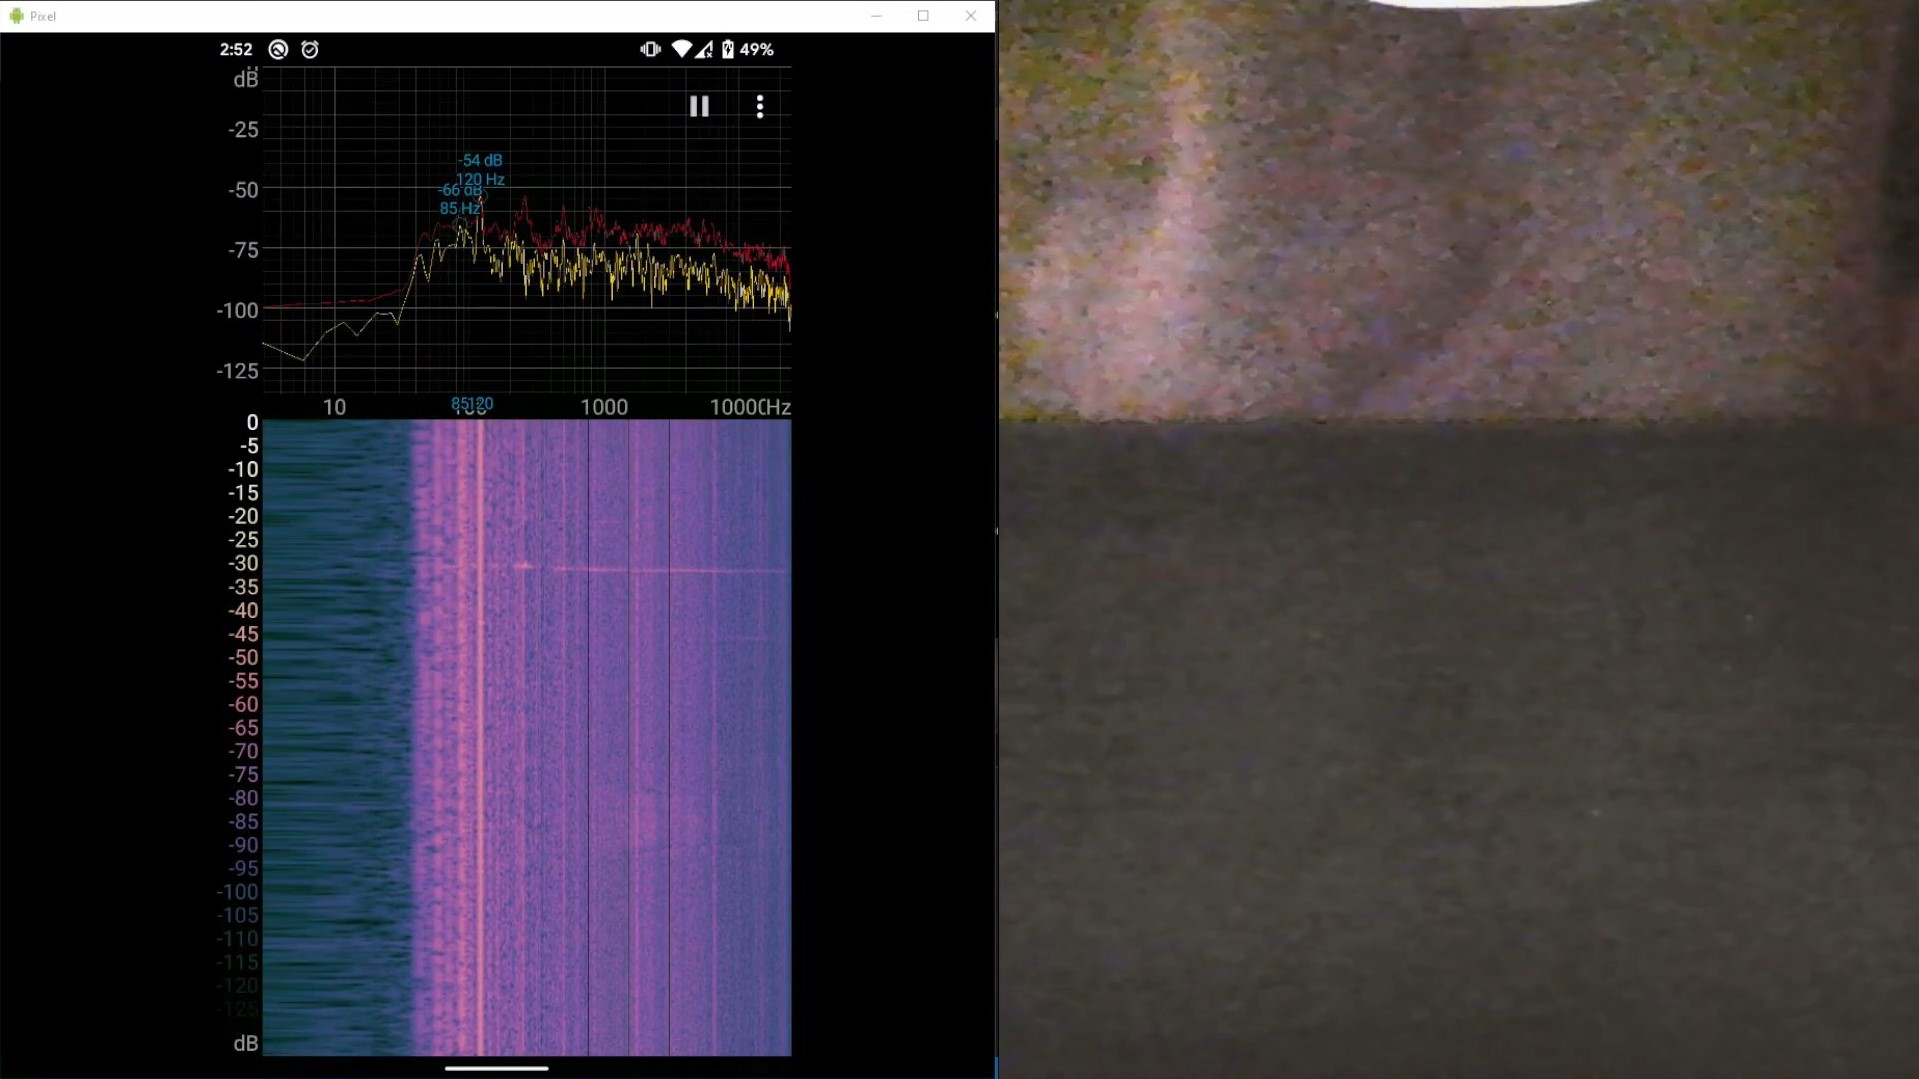
\includegraphics[width=.90\linewidth]{Figures/4 Protocol Design/Signal to Noise Ratio/silent_background_noise.jpg}
        \caption{Silent Room}
        \label{fig:signal-to-noise-ratio-silent}
    \end{subfigure}%
    \begin{subfigure}{.50\textwidth}
        \centering
        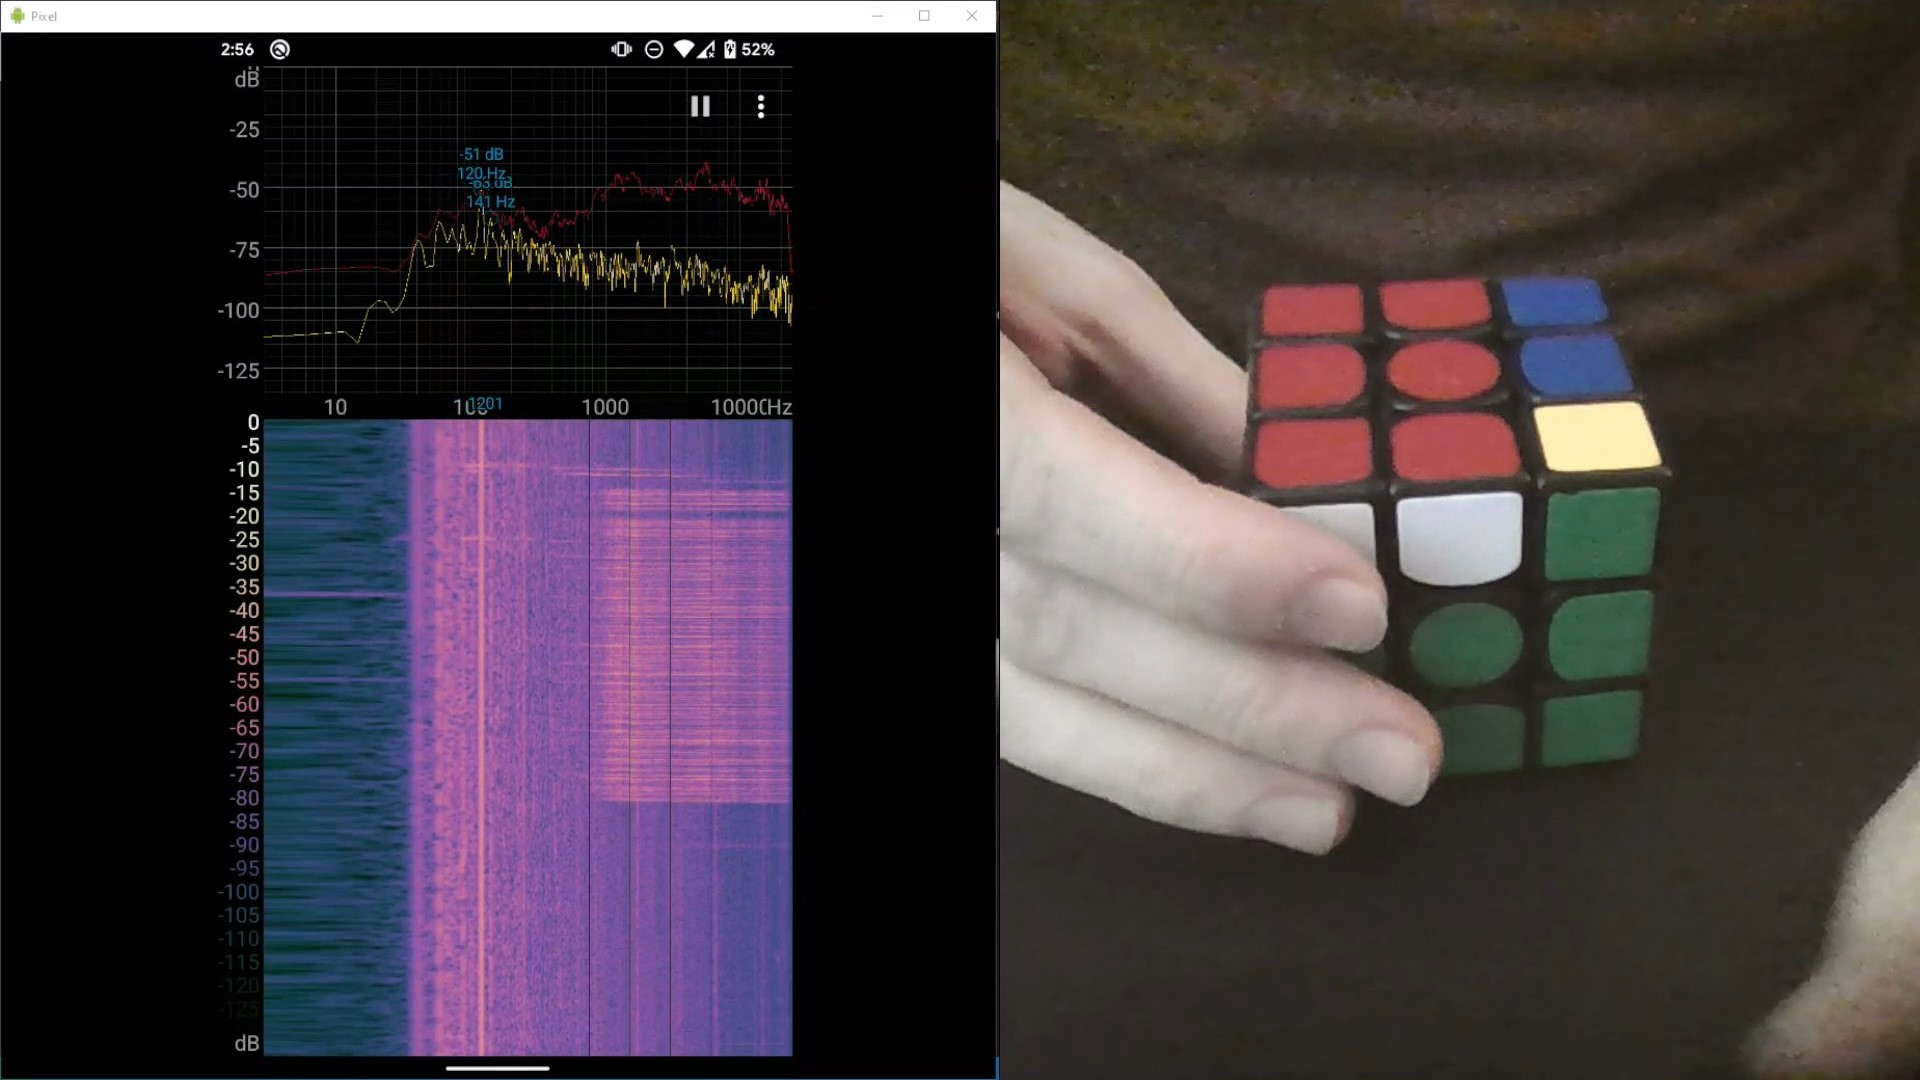
\includegraphics[width=.90\linewidth]{Figures/4 Protocol Design/Signal to Noise Ratio/356_background_noise.jpg}
        \caption{Quiet Solving (Gans 356)}
        \label{fig:signal-to-noise-ratio-356}
    \end{subfigure}\\%
    \begin{subfigure}{.50\textwidth}
        \centering
        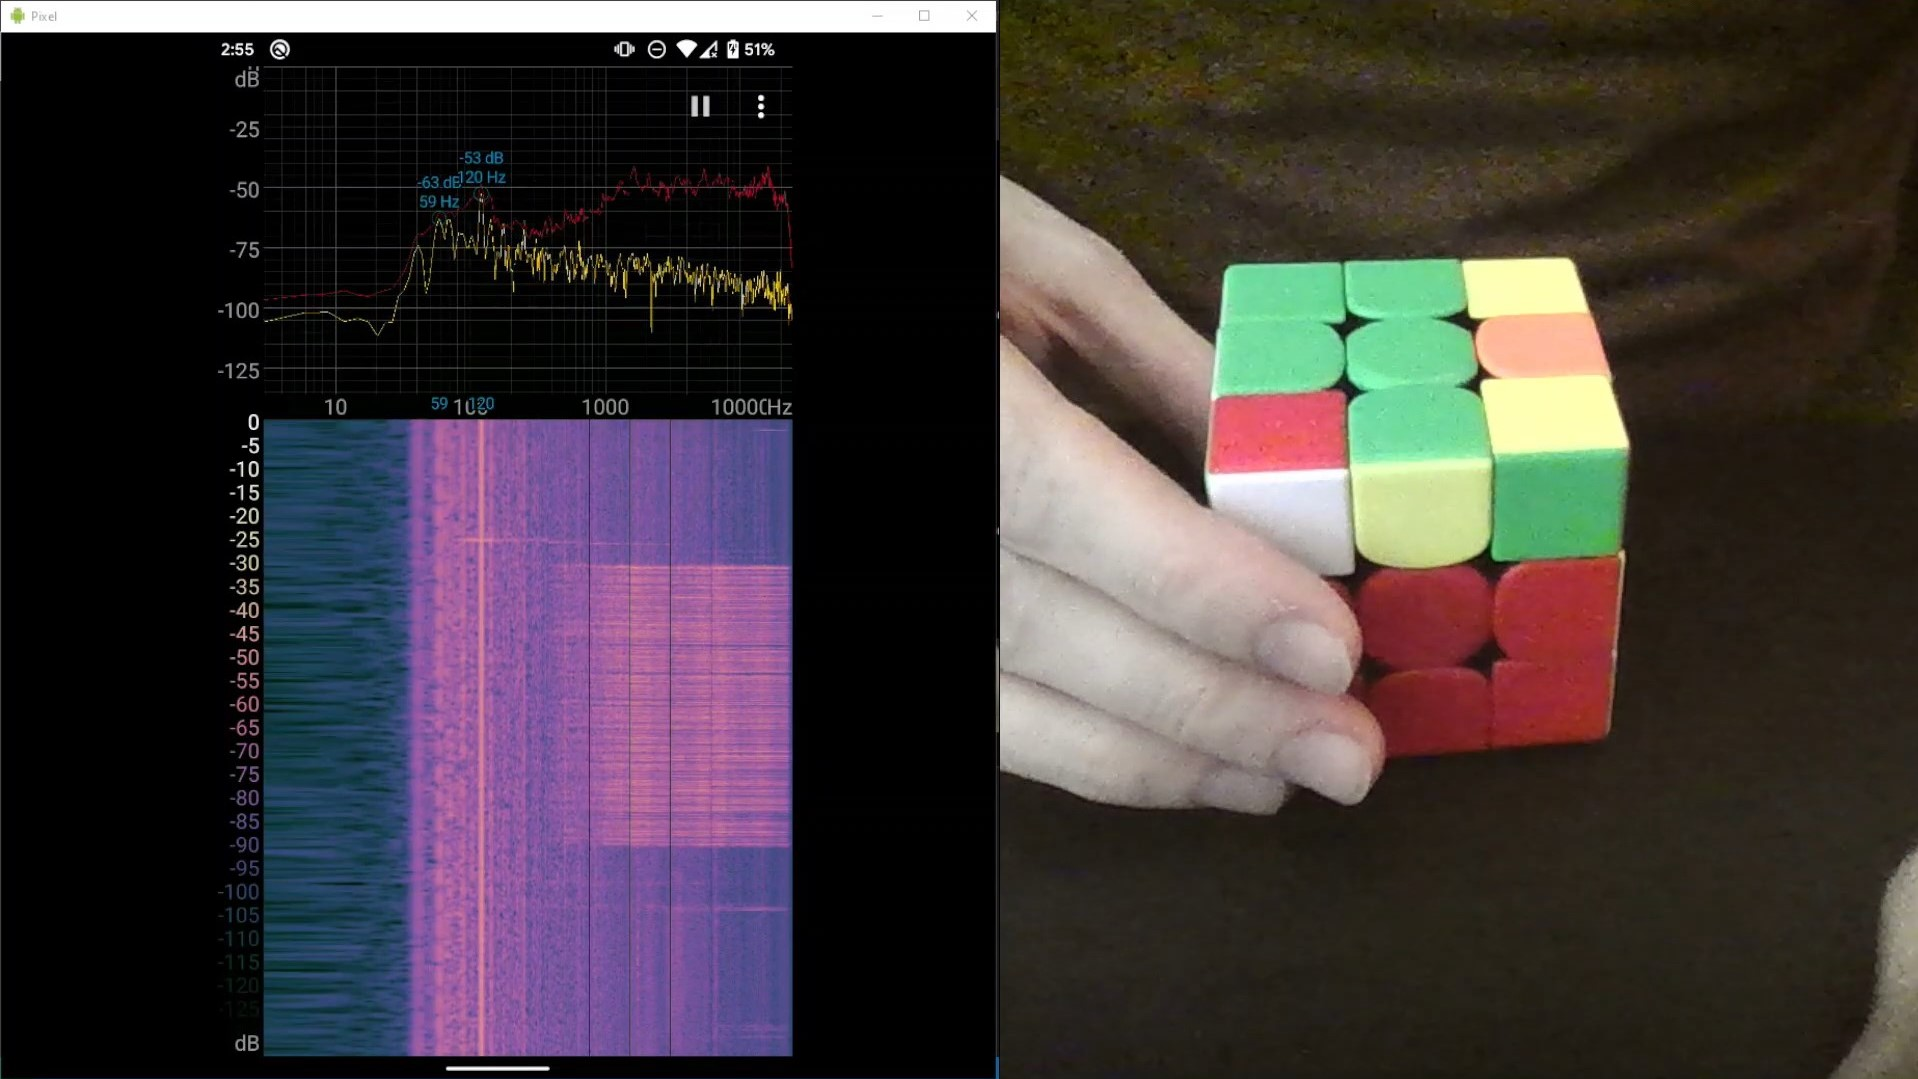
\includegraphics[width=.90\linewidth]{Figures/4 Protocol Design/Signal to Noise Ratio/xs_background_noise.jpg}
        \caption{Normal Solving (Gans XS)}
        \label{fig:signal-to-noise-ratio-xs}
    \end{subfigure}%
    \begin{subfigure}{.50\textwidth}
        \centering
        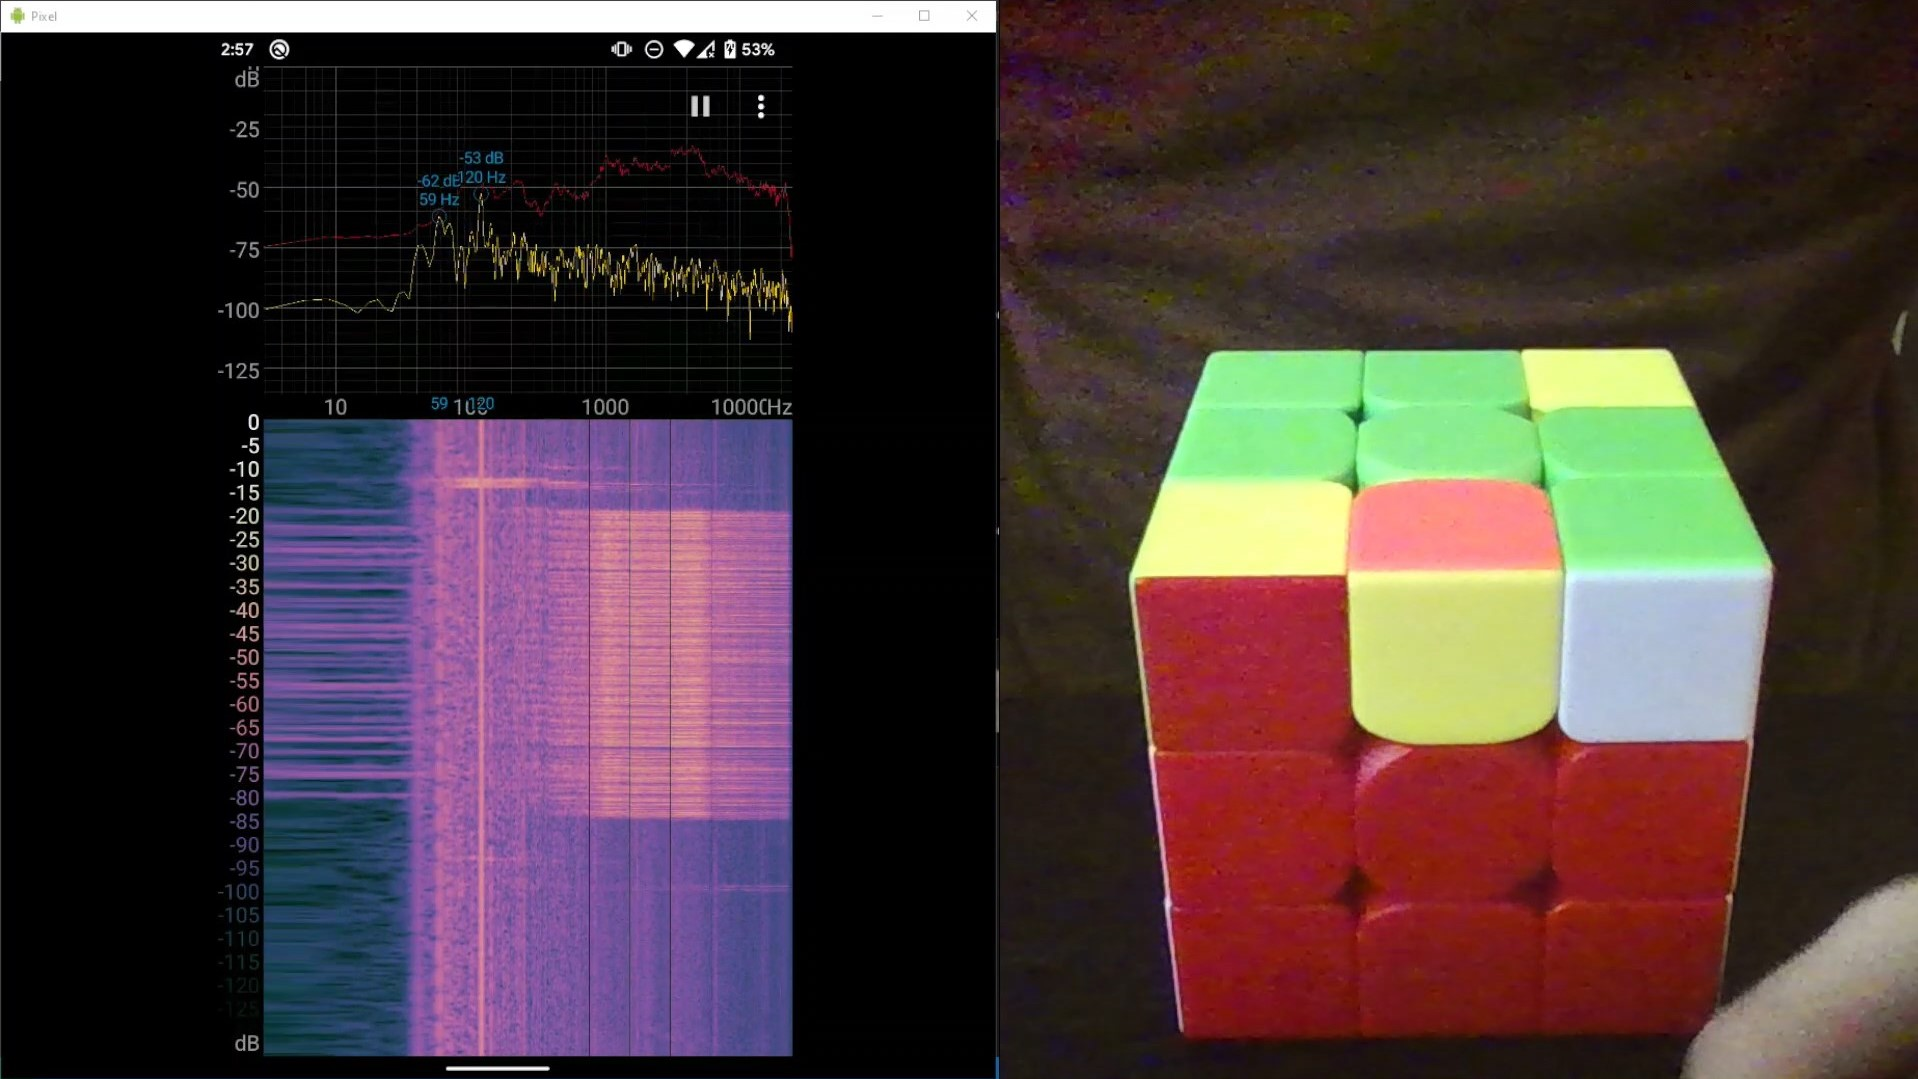
\includegraphics[width=.90\linewidth]{Figures/4 Protocol Design/Signal to Noise Ratio/qiyi_background_noise.jpg}
        \caption{Loud Solving (QiYi Qimeng)}
        \label{fig:signal-to-noise-ratio-qiyi}
    \end{subfigure}%
    \caption{The background noise of a quiet room compared to solving several speedcubes}
    \label{fig:signal-to-noise-ratio}
\end{figure}

As shown in Figure ~\ref{fig:signal-to-noise-ratio}, the predominant background noises in a "quiet" room are the tones between 80Hz - 500Hz which reach a max strength of -54dB.
In contrast, the background noise of solving a speedcube spans all the way from 1000Hz - 20000Hz, with particular strength from the noisy QiYi cube in the 1000Hz - 10000Hz range reaching up to -30dB.

Thus, a sound-based move tracking protocol must account for the following items in order to achieve an adequate signal-to-noise ratio:
\begin{itemize}
    \item Tones between 500Hz and 1000Hz are the easiest to detect while solving a speedcube.
    \item Tones between 1000Hz and 20000Hz must be significantly louder than -30dB to be properly detected.
\end{itemize}

\subsection{Tone Distinctiveness}
\label{subsec:tone-distinctiveness}
If more than one tone is required for the protocol, each tone must be unique enough to be easily distinguished from each other tone.
Since a standard smartphone or laptop microphone will be used on the listening end of this protocol, the definition of "easily distinguishable" must be based on an assessment of how clearly smartphone and laptop-grade microphones can distinguish similar frequencies.

To measure the sensitivity of a standard smartphone microphone (in this case a Google Pixel 1), a recording was taken of two distinct tones that started 500 Hz apart and stepped closer together in 10 Hz increments every 0.5 seconds until their frequencies were identical.

% How to do a sub-figure: https://tex.stackexchange.com/a/37597
\begin{figure}[h]
    \centering
    \begin{subfigure}{0.33\textwidth}
        \centering
        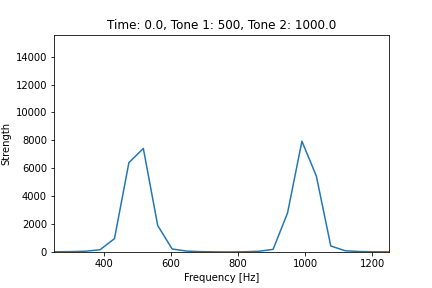
\includegraphics[width=.90\linewidth]{Figures/4 Protocol Design/Tone Distinctiveness/0.06.png}
        \caption{500Hz Separation}
        \label{fig:tone-sep-500}
    \end{subfigure}%
    \begin{subfigure}{0.33\textwidth}
        \centering
        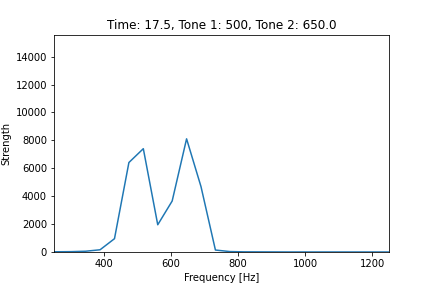
\includegraphics[width=.90\linewidth]{Figures/4 Protocol Design/Tone Distinctiveness/17.53.png}
        \caption{150Hz Separation}
        \label{fig:tone-sep-150}
    \end{subfigure}%
    \begin{subfigure}{0.33\textwidth}
        \centering
        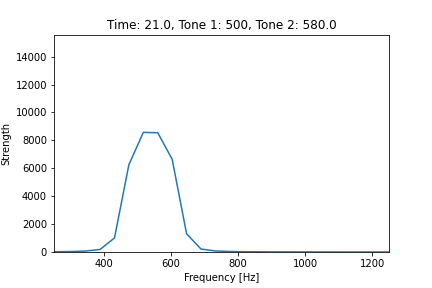
\includegraphics[width=.90\linewidth]{Figures/4 Protocol Design/Tone Distinctiveness/21.01.png}
        \caption{80Hz Separation}
        \label{fig:tone-sep-80}
    \end{subfigure}%
    \caption{As two tones get more similar, they get harder to distinguish, particular when fewer than 100Hz apart.}
    \label{fig:tone-sep}
\end{figure}

As shown in Figure ~\ref{fig:tone-sep}, the two tones are clearly distinguishable from 500Hz apart to 150Hz apart.
However, once the tones came within 80Hz of each other, they became entirely indistinguishable.

Thus, a sound-based move tracking protocol must account for the following items in order to achieve adequate tone distinctiveness:
\begin{itemize}
    \item Tones must be separated by at least 100Hz in order to be clearly distinguished from other tones in the protocol.
\end{itemize}


\subsection{Frequency Response Range of Consumer Hardware}
\label{subsec:frequency-response-range}
Since a standard smartphone or laptop microphone will be used on the listening end of this protocol, any tones used in the protocol must be within the range of tones that a smartphone or laptop-grade microphones can pick up.
This range is formally known as the "frequency response range" of the microphone.

According to a Stanford research paper that analyzed over 10,000 mobile devices, the typical smartphone microphone has a frequency response range of 20Hz to 20kHz as shown in Figure ~\ref{fig:freq-res-range}

\begin{figure}[h]
    \centering
    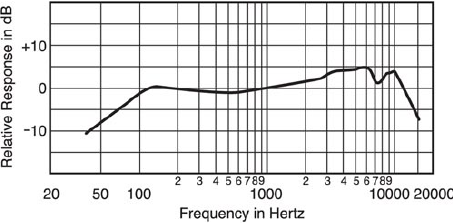
\includegraphics[width=.50\linewidth]{Figures/4 Protocol Design/Frequency Response Range/typical-smartphone-response-range.png}
    \decoRule
    \caption{"A typical frequency response curve for a microphone." \cite{typical-mic-range}}
    \label{fig:freq-res-range}
\end{figure}

Thus, a sound-based move tracking protocol must account for the following restrictions on which tones can be used for the protocol:
\begin{itemize}
    \item Tones used in the protocol must fall on the range of 20Hz-20kHz in order to be detectable by a typical smartphone or laptop microphone.
\end{itemize}

\subsection{Human Auditory Range}
\label{subsec:human-auditory-range}
An audible protocol could be distracting to a speedcuber. 
The human ear can detect audible frequencies from 20Hz to 20kHz, though this usually degrades with age with many people unable to notice sounds above 16kHz. \cite{audible-range}.
However, not all tones are pleasant to listen to, particularly higher frequency tones.
Tones within the frequency range of a piano (27.5Hz - 4kHz) are generally considered acceptable, while tones above the piano's upper range are often irritating. \cite{piano-range}

Thus, a sound-based move tracking protocol should be considerate of the human ear's sensitivity to various frequencies:
\begin{itemize}
    \item The most acceptable tones for human speedsolvers are in the musical range of up to 4kHz or above the standard audible range of 16kHz
\end{itemize}


\section{Specification}
\label{sec:specification}
Given the above constraints, this section will detail a sound-based protocol for tracking the moves of a Rubik's Cube by continuously transmitting the current state of the cube. In this protocol, changes to the cube's state cause a change in the transmitted tones which can be recorded and analyzed to determine the face turn applied.

\subsection{Representing the Cube's Current State}
\label{subsec:representing-cube-state}
As mentioned in Section \ref{sec:rubiks-anatomy}, a Rubik's Cube has six centerpieces that are fixed relative to each other, but can each rotate freely through four possible rotational positions as shown in Figure \ref{fig:rotation-alignment}.

\begin{figure}[h]
    \centering
    \begin{subfigure}{0.25\textwidth}
        \centering
        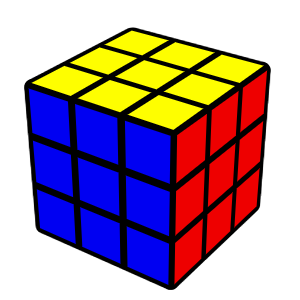
\includegraphics[width=.90\linewidth]{Figures/4 Protocol Design/Specification/fully-aligned.png}
        \caption{Full Alignment}
        \label{fig:rotation-aligned}
    \end{subfigure}%
    \begin{subfigure}{0.25\textwidth}
        \centering
        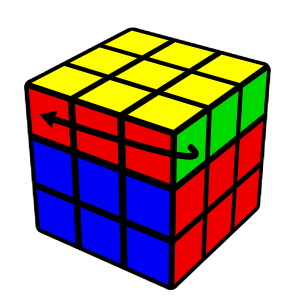
\includegraphics[width=.90\linewidth]{Figures/4 Protocol Design/Specification/90_misaligned.png}
        \caption{90$^\circ$ Misalignment}
        \label{fig:rotation-misaligned-90}
    \end{subfigure}%
    \begin{subfigure}{0.25\textwidth}
        \centering
        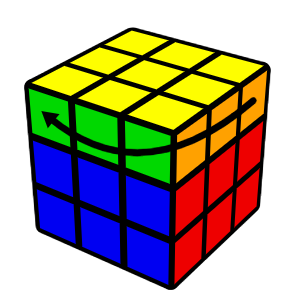
\includegraphics[width=.90\linewidth]{Figures/4 Protocol Design/Specification/180_misaligned.png}
        \caption{180$^\circ$ Misalignment}
        \label{fig:rotation-misaligned-180}
    \end{subfigure}%
    \begin{subfigure}{0.25\textwidth}
        \centering
        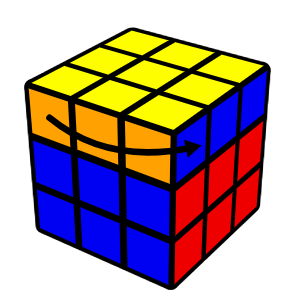
\includegraphics[width=.90\linewidth]{Figures/4 Protocol Design/Specification/270_misaligned.png}
        \caption{270$^\circ$ Misalignment}
        \label{fig:rotation-misaligned-270}
    \end{subfigure}%
    \caption{Each face of the Rubik's Cube can occupy one of four rotational positions at any given time (Pictures from \cite{rubiks-turns-images})}
    \label{fig:rotation-alignment}
\end{figure}

The state of a centerpiece is defined as its current rotational position. 
Implicit in this definition is the fact that a centerpiece is guaranteed to occupy one and only one of its four possible states at any given time.

Each of the six centerpieces has an independent set of four possible states, yielding a total of 24 different centerpiece states for the Rubik's Cube, of which there will always be exactly six active at any given time.

It's important to note that a knowledge of the current state of each centerpiece does not imply knowledge of the exact state of each of edge and corner cubie.
For example, after applying the algorithm R U R' U' all centerpieces have the same state they occupied prior to the algorithm's execution while, most of the edges and corners in the R and U layers will have been moved or rotated.
However, in the reverse case, knowledge of the applied move sequence is sufficient information to determine the exact state of all cubies.
Section \ref{subsec:tracking-face-turns} will explain how extract full move sequences using only the state information of the centers.

\subsection{Tracking Face Turns}
\label{subsec:tracking-face-turns}
The only way to change a centerpiece's state is by applying a face turn.
As such, when a centerpiece is rotated to a new position, its state changes to that of the new position.
From there, a simple comparison of the new state to the previous state reveals the exact face turn applied to the cube.

Thus, in order to determine the sequences of moves applied to the Rubik's Cube, one simply needs to track how the state of its centerpieces changes over time. 

\subsection{Conveying State Through Sound}
\label{subsec:conveying-state-through-sound}
Conveying the current state of the cube's centerpieces through sound can be done by simply associating each of the 24 possible centerpiece states with a specific tone and broadcasting a signal composed of the six tones corresponding to the active states of the cube's centerpieces.
Whenever a face turn is applied, the tone associated with the rotated centerpiece would change to the tone representing the piece's new state.
From there, a microphone equipped device can record the broadcast frequencies, measure the changes in the frequencies over time, convert the frequency changes to state changes, and finally extract any move sequence applied to the cube.


\section{Alternatives}
\label{sec:alternatives}
% \subsection{Relative Sound Positioning}
% \label{subsec:relative-sound-positioning}
Instead of transmitting the current state of the cube's centerpieces, an alternative protocol design could seek to directly transmit the face turns applied to the cube.

This perspective focuses on the fact that all move sequences can be broken down into a series of 90$^\circ$ face turns.
Since the cube consists of 6 faces, and each face can be turned either clockwise or counterclockwise, one could design a two-tone protocol using only 8 discrete audio frequencies to build the smart cube.
The first tone would come from one of six predefined audio bands, one for each face of the cube. 
The second tone would come from one of two separately predefined audio bands, one for each possible direction of rotation.
From this, an audio processing model could be designed to process a sequence of these two-tone pairs and reconstruct the sequence of face rotations by recording the rotated face followed by its direction of rotation.

However, while this model minimizes the number of discrete frequencies required to communicate changes in the cube's state, it carries many challenges.
Consider the example of a speedcuber averaging 5 turns per second (common for a 12-15 second solver) with bursts up to 10 TPS.
The burst TPS would require the successful transmission of 20 sequential tones within a single second - only 50ms per tone, all in the midst of additional noise from the cube's pieces hitting each other harder at the higher turn speed.
Adding to the difficulty, since each tone is only ever transmitted once, the audio detection model must achieve 100\% tone recognition to be able to accurately reconstruct the originating move sequence.
As a result, this model fails to support any sort of error correction that would make it resistant to the common challenges to data transmission through sound.
 
% Chapter Template

\chapter{Audio Decoding Algorithm Design} % Main chapter title

\label{Chapter5} % Change X to a consecutive number; for referencing this chapter elsewhere, use \ref{ChapterX}


\section{Synthetic Audio Generation}

Prior to investing significant resources in PCB design, we found it prudent to develop a synthetic model of the ideal audio output of the DIY Supercube. This model consists of a synthetic audio generator that, when given a specific move sequence, generates a `.wav` file consisting of the distinct time series tones that the DIY Supercube would theoretically produce. The synthetic data produced by this model then served as the first test cases for the final audio decoding model.

\subsection{Representing the Audio Protocol}
TODO pull from Jupyter notebook

\subsection{Representing the Rubik's Cube}
TODO pull from Jupyter Notebook

\subsection{Generating the Audio for an Arbitary Algorithm}
TODO pull from Jupyter Notebook

TODO show a spectrogram of the generated audio here


\section{Decoding the Synthetic Audio}

TODO pull from Jupyter Notebook

\subsection{Examining the Waveform}
TODO pull from Jupyter Notebook

\subsection{Conversion to Strength of Individual Frequencies}
TODO pull from Jupyter Notebook


\section{Adding Realisitic Noise to the Synthetic Audio}

TODO pull from Jupyter Notebook


\section{Decoding the Noisy Synthetic Audio}

TODO pull from Jupyter Notebook

\subsection{Optimizing algorithm parameters}
TODO - Share the strategy for finding the optimal parameters, and the end results, but defer the detailed analysis for the Evaluation.
 
% Chapter Template

\chapter{The Transmitter} % Main chapter title
\label{Chapter6} 


\section{Introduction}

The transmitter for the sound-based move tracking protocol is in charge
of creating the tones representing each centerpiece's current state,
and updating those tones each time a centerpiece changes state.

This chapter will detail a proof-of-concept design for a printed
circuit board (PCB) containing only nine discrete components capable of
generating all the tones required for encoding one centerpiece's state.

This chapter assumes that the reader has a knowledge of basic circuit
components like resistors and capacitors. It begins with a
discussion of the requirements/constraints for the physical transmitter
(Section \ref{sec:transmitter-requirements}) and an experiment
analyzing the effects of various sound obstructions on signal strength
(Section \ref{sec:minimizing-sound-obstruction}). From there a formal
design schematic for the transmitter will be presented (Section
\ref{sec:transmitter-design}) and prototyped (Sections
\ref{sec:prototype} and \ref{sec:miniaturization})


\section{Requirements}
\label{sec:transmitter-requirements}

This section will detail the constraints within which the transmitter
will be required to operate. These constraints include the physical
size of the transmitter (Section
\ref{subsec:prospects-of-miniaturization}), the precision of tone
generation (Section \ref{subsec:precision-of-tone-generation}), the
reliability of the transmitter in changing tones to reflect a face turn
(Section \ref{subsec:responsiveness-to-face-turns}), and the intensity
of output audio that the transmitter can produce (Section
\ref{subsec:transmitter-signal-to-noise-ratio}).

\subsection{Prospects of Miniaturization}
\label{subsec:prospects-of-miniaturization}

The transmitter must be both removable and small enough to fit in the
center cap of each face of a speedcube. This requirement stems from two
sources. First, in contrast to all existing smartcubes, most
non-smartcubes have small, solid cores (Figure
\ref{fig:356-core-closed}) that provide no extra space for the
inclusion of any electronics, but do have a small amount of open space
within their center cubies (Figure \ref{fig:356-core-open}). Second,
the use of a cube with non-removable, embedded electronics violates the
WCA competition regulation 2i \cite{wca-regulations} (See also Section
\ref{subsec:competition-regulations}).

\begin{figure}[h]
    \centering
    \caption{Internal pieces of a standard speedcube (Gans 356)}
    \label{fig:356-core}
    \begin{subfigure}{.45\textwidth}
        \centering
        \caption{View of the small, solid plastic core}
        \label{fig:356-core-closed}
        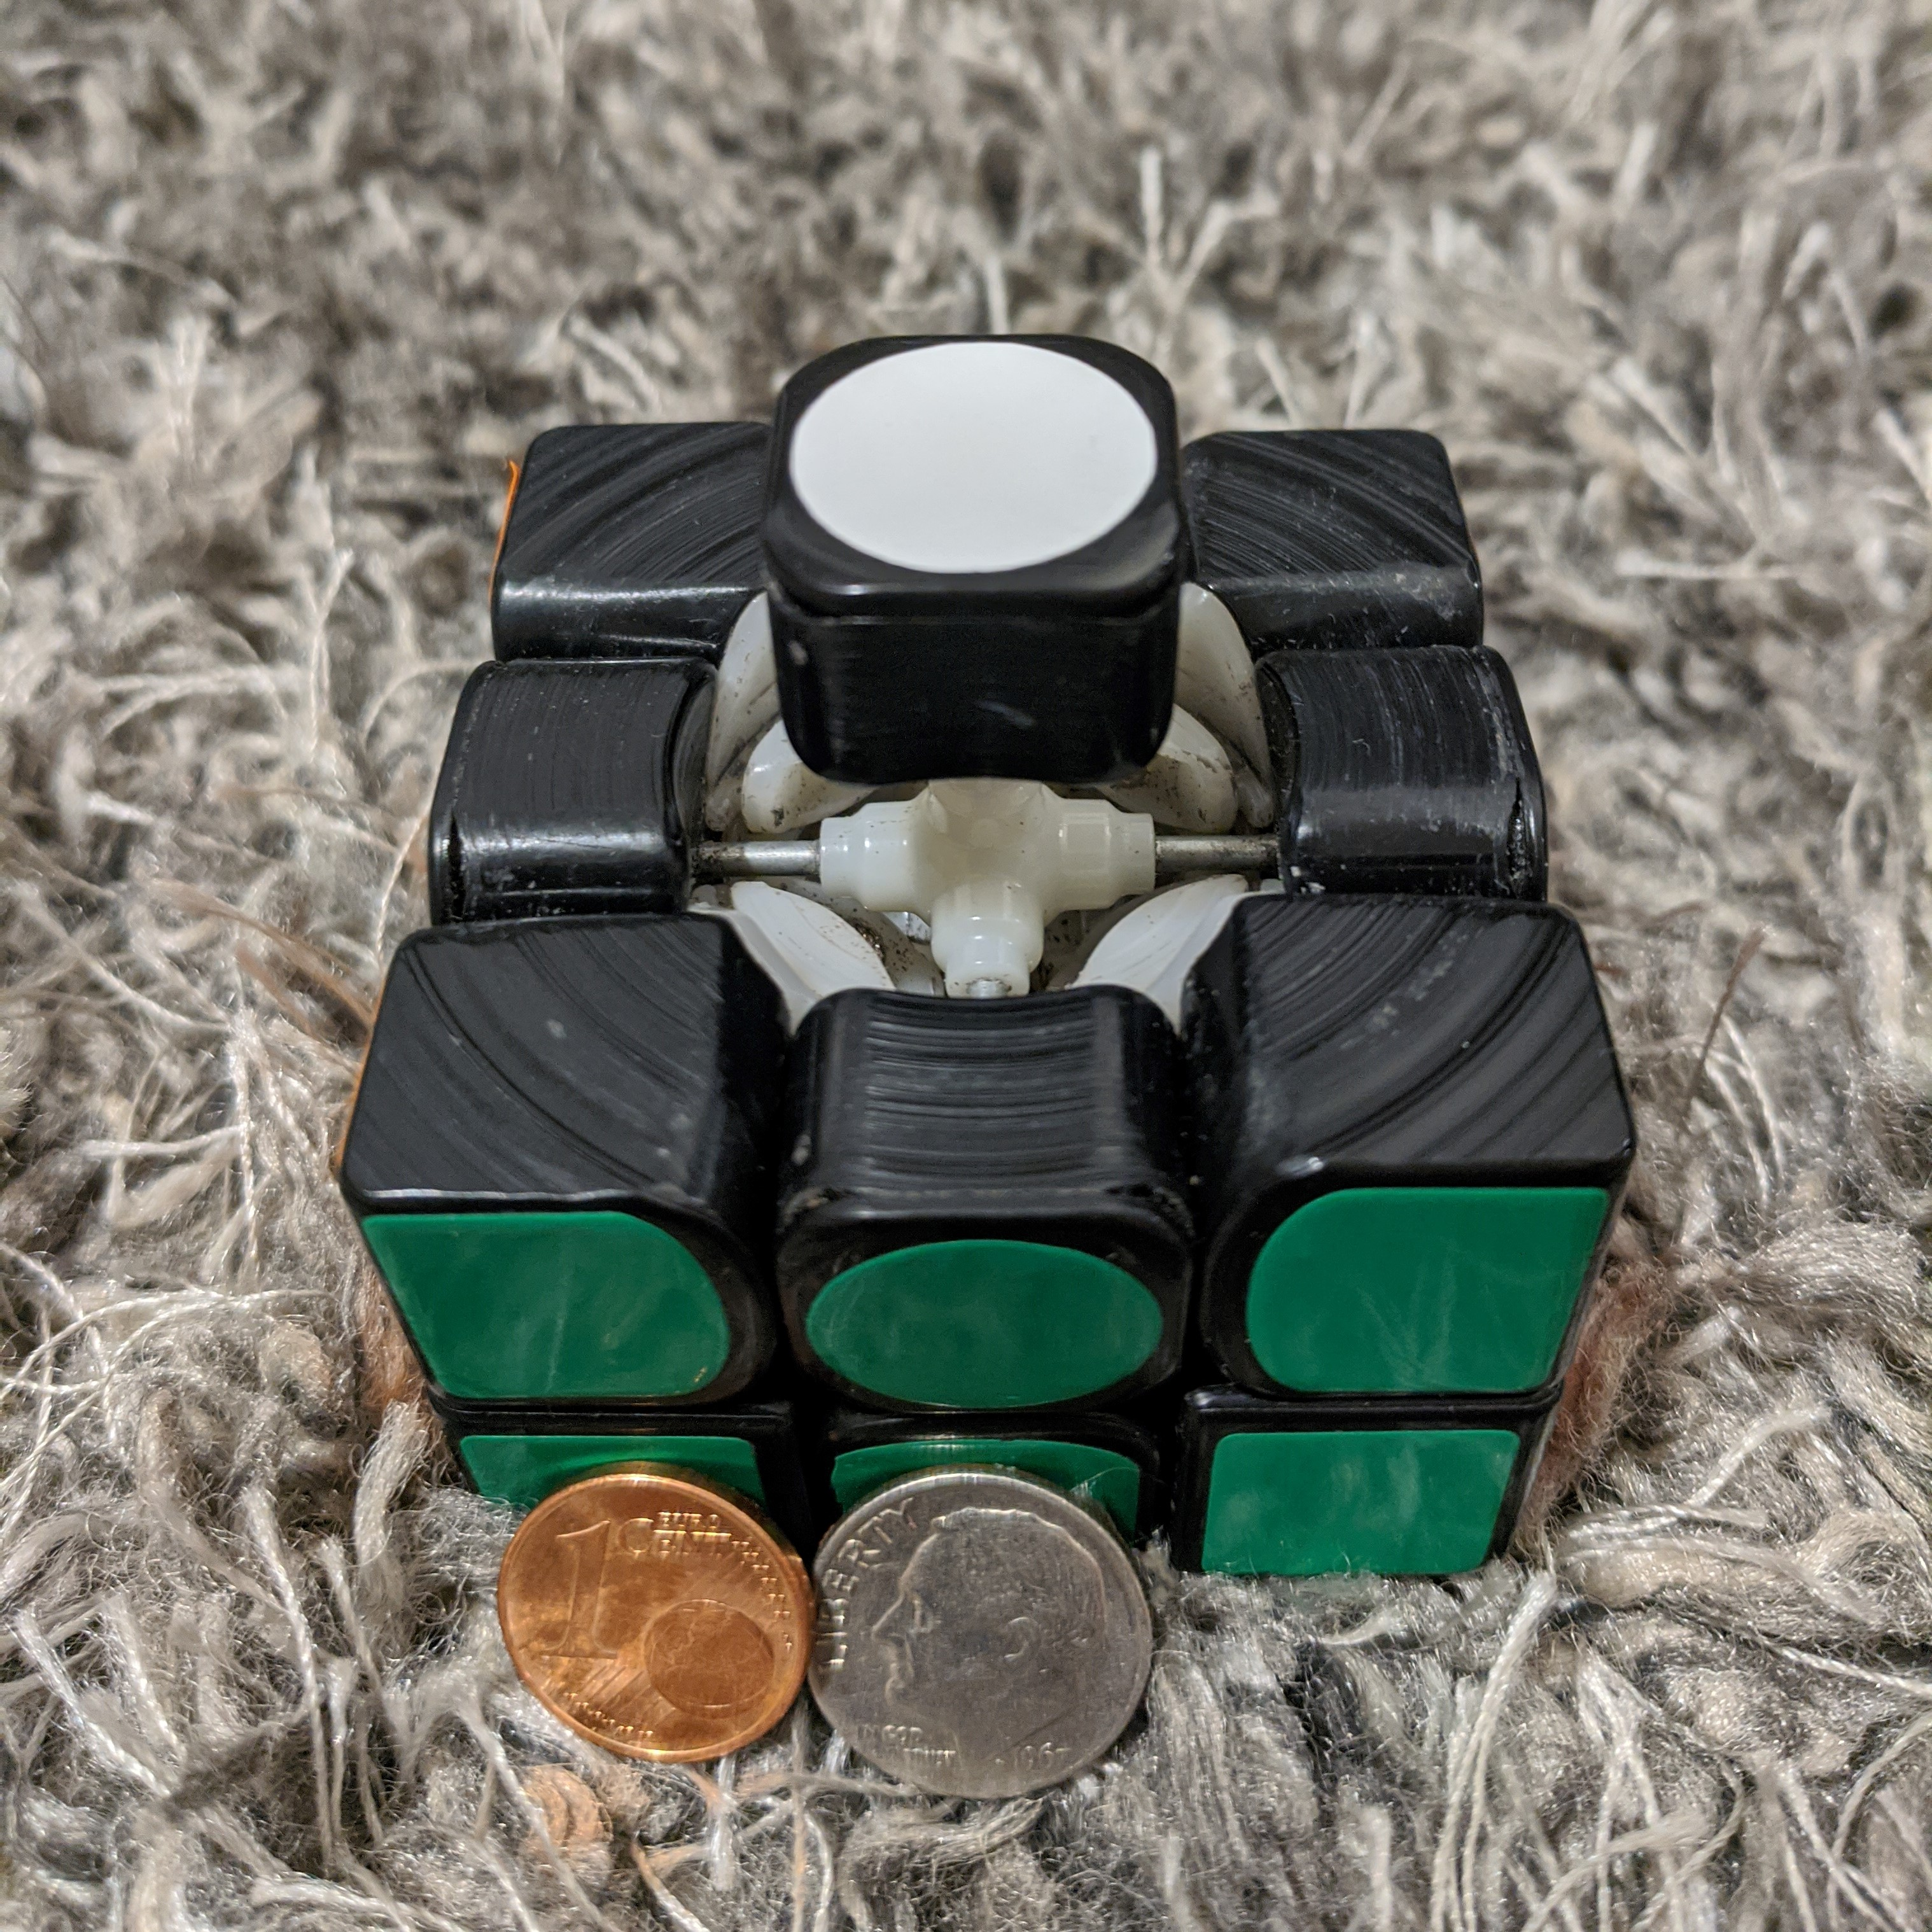
\includegraphics[width=\linewidth]{Figures/6 PCB Design/356_core_cropped.jpg}
    \end{subfigure}
    \begin{subfigure}{.45\textwidth}
        \centering
        \caption{View of the space inside the centerpiece}
        \label{fig:356-core-open}
        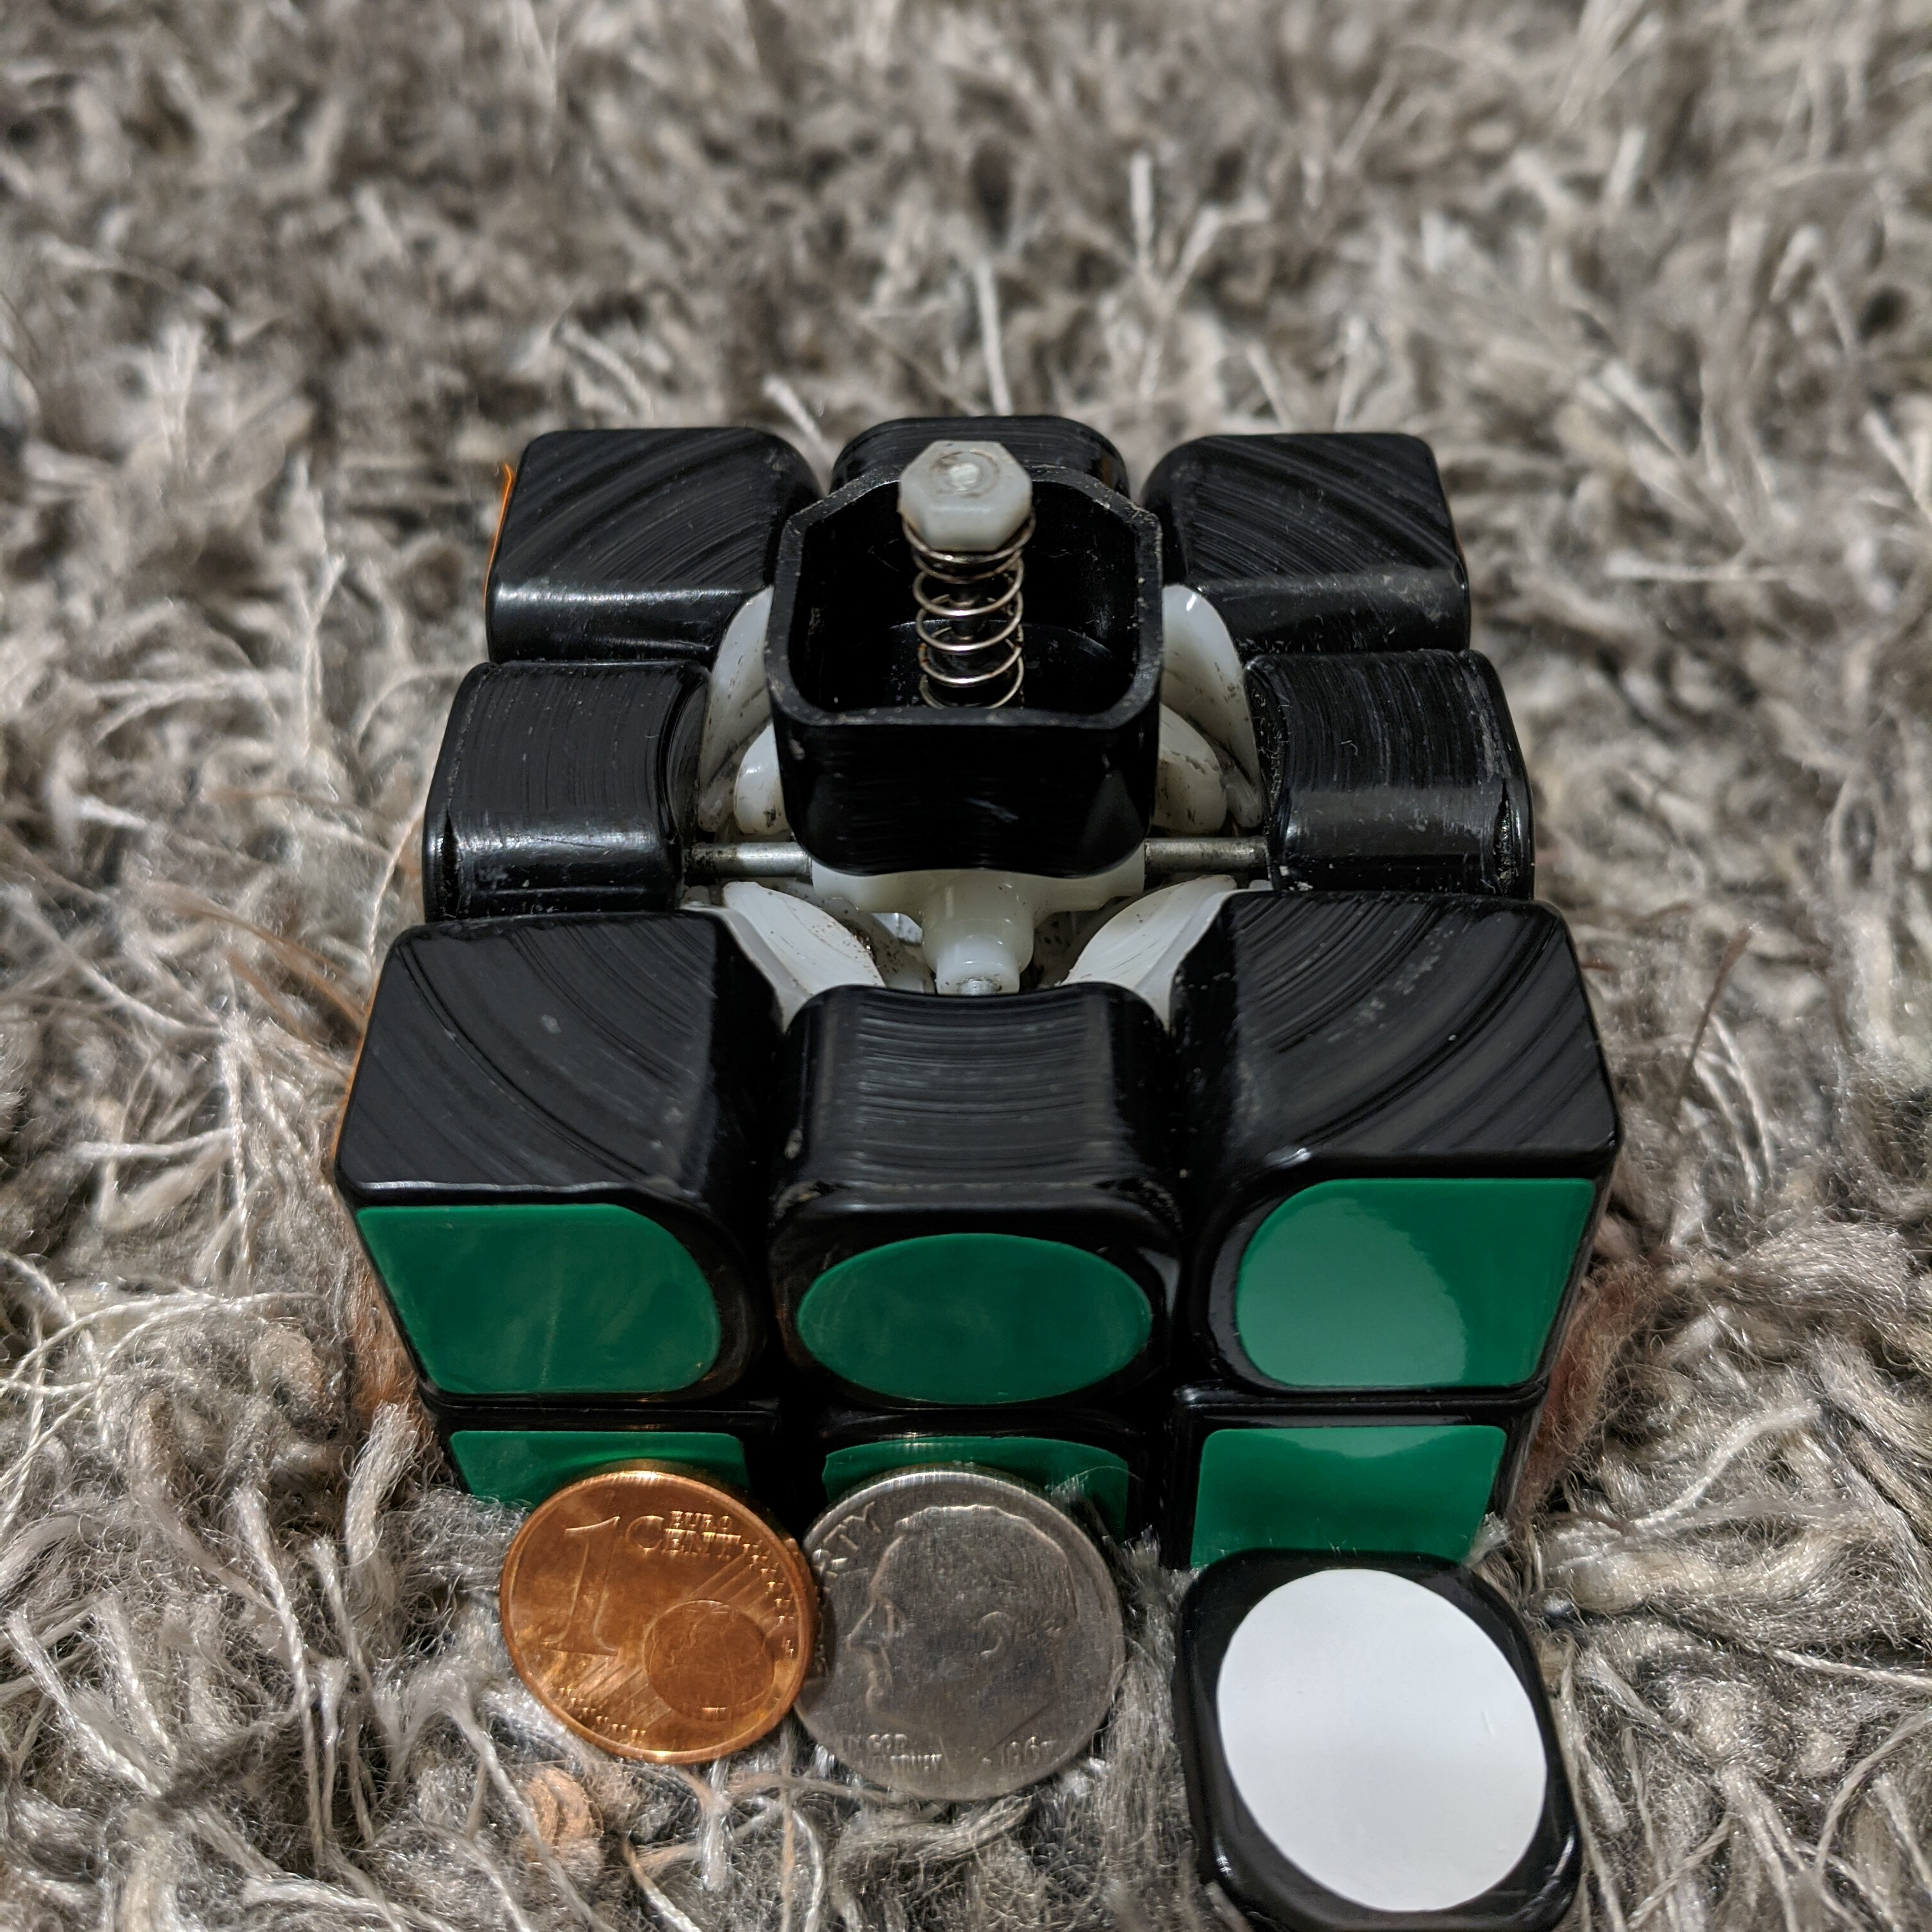
\includegraphics[width=\linewidth]{Figures/6 PCB Design/356_core_open_cropped.jpg}
    \end{subfigure}
\end{figure}

\subsection{Precision of Tone Generation}
\label{subsec:precision-of-tone-generation}

While the receiver specified in Chapter \ref{Chapter5} supports custom
state to frequency mappings, it expects that the frequency
corresponding to each centerpiece's state stays constant throughout the
entire audio recording. As such, the chosen transmitter design can
encode centerpiece states with any frequency (assuming the chosen
frequencies work within the constraints specified in Section
\ref{sec:protocol-requirements}), but it must produce its chosen
frequencies with high precision.

\subsection{Responsiveness to Face Turns}
\label{subsec:responsiveness-to-face-turns}

The chosen transmitter design must respond to an applied face turn by
changing the currently transmitted audio frequency to the frequency
corresponding to the new centerpiece state. Since top speedcubers can
reach a burst turn speed of 20 TPS (see Section
\ref{sec:alternatives}), this means this frequency change must complete
within 50ms.

\subsection{Signal-to-Noise Ratio}
\label{subsec:transmitter-signal-to-noise-ratio}

The transmitter must create tones loud enough to be easily
distinguished from ambient noise, including the sound of the Rubik's
Cube's own turns. In light of the above requirement for the transmitter
to fit within a center cubie
(\ref{subsec:prospects-of-miniaturization}), this requirement will also
require the transmitter design to consider how to overcome any audio
dampening caused by such an enclosure.


\section{Minimizing Sound Obstruction}
\label{sec:minimizing-sound-obstruction}

Section \ref{subsubsec:key-observations-from-the-spectrogram} talks
about the noise levels from various speedcubes. Constrast with the
noise levels produced here to show validity.

TODO Discuss the "tupperware" tests -> design of various center caps.

Voluptate labore quis aliqua laboris nulla reprehenderit ea incididunt
fugiat. Tempor ea ipsum in quis incididunt quis dolor pariatur ad
cillum irure ad aliquip aliqua. Mollit proident officia id excepteur.

Ut officia sit et consectetur reprehenderit nostrud consectetur. Nulla
culpa magna consequat elit excepteur. Nisi nisi ipsum reprehenderit
nisi commodo sit pariatur labore cupidatat cillum ullamco ut mollit.
Nostrud ipsum anim commodo ipsum sunt id consequat. Ex ut ullamco ea
exercitation est ad commodo est.

\section{Design}
\label{sec:transmitter-design}

Given the above constrains, this section will detail a design for a
printed circuit board capable of precisely generating four distinct
tones.

\subsection{The 555 Timer}
\label{sec:the-555-timer}

The core component in this PCB design is a 555 timer, which is a
computer chip that facilitates the generation of many types of voltage
frequencies in a circuit.

For this transmitter, the 555 timer will be configured to output a
square wave voltage signal with a 50\% duty cycle (i.e. "Astable
Operation") \cite{icm7555}. This means the voltage on the output pin
will alternate between low and high, spending equal amounts of time in
each state.

The attentive reader will notice that the square wave signal proposed
here differs from the sine wave used to create the synthetic audio in
Figure \ref{fig:code-generate-alg-audio}. Valid concerns may even be
raised about the fact that a square wave is actually a composite of a
fundamental sine wave and infinitely many harmonics \cite{harmonics}.
However, since the nearest harmonic in a square wave with a 50\% duty
cycle oscillates at a frequency three times as fast as the fundamental
\cite{square-waves}, then choosing a fundamental frequency of at least
6.67kHz places the nearest harmonics beyond the range of frequencies
measurable by a typical smartphone or laptop microphone (see Section
\ref{subsec:frequency-response-range}).

The standard schematic for creating this type of voltage signal is
depicted in Figure \ref{fig:555_astable}.

\begin{figure}[h]
    \centering
    \caption{Standard 555 Timer Circuit for Astable Operation \cite{icm7555}}
    \label{fig:555_astable}
    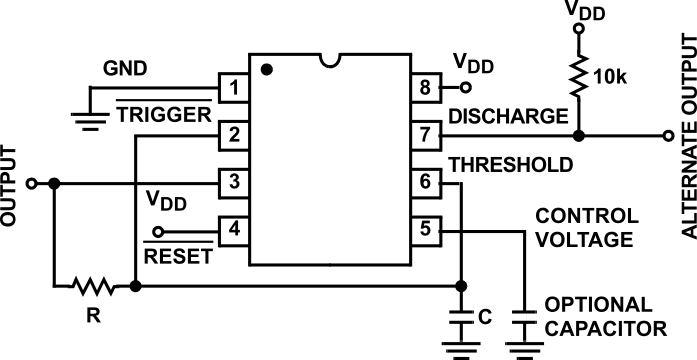
\includegraphics[width=0.75\linewidth]{Figures/6 PCB Design/555_astable.png}
\end{figure}

The two key components are the resistor \code{R} and the capacitor
\code{C} whose respective resistance and capacitance control the output
frequency \code{f} via the relation shown in Equation \ref{eq:555-freq}
\cite{icm7555}:

\begin{equation}\label{eq:555-freq}
    f = \frac{1}{1.4 R C}
\end{equation}

\subsection{Creating Audio}

The 555 timer's varying voltage output can be easily converted to
audible sound by attaching a voltage controlled speaker to the output
wire coming from pin 3 in Figure \ref{fig:555_astable}. However, this
will only produce one continuous tone, and each centerpiece will need
to be able to switch between four distinct tones. As such, the resistor
\code{R} will need to be replaced with four separate resistors (labeled
\code{R1}, \code{R2}, \code{R3}, \code{R4} in Figure
\ref{fig:555_astable_modded}) and a switch. The switch will be
connected to the cube so that a 90$^\circ$ rotation will change which
resistor is in series with the circuit, thus changing the output audio
frequency of the speaker.

\begin{figure}[h]
    \centering
    \caption{Centerpiece State Transmitter Circuit}
    \label{fig:555_astable_modded}
    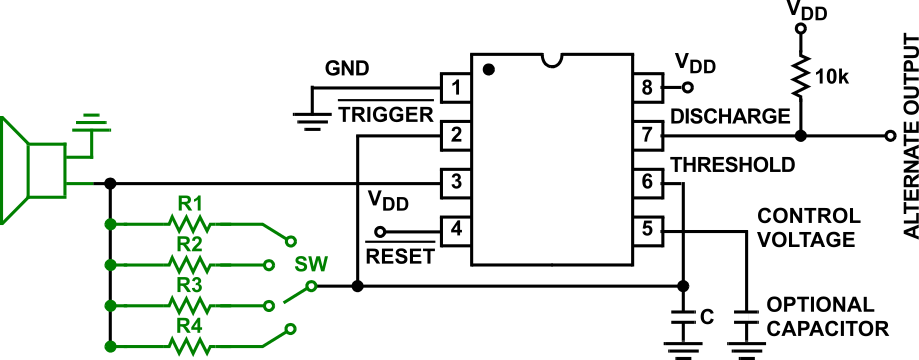
\includegraphics[width=\linewidth]{Figures/6 PCB Design/555_astable_modded.png}
\end{figure}

Alternatively, it is mathematically valid to instead switch between
four different capacitors of different capacitance. However, for the
reasons described in Section \ref{subsec:freq-selection}, opting to
switch between resistors proved more practical.

\subsection{Choosing the values of \code{R} and \code{C}}
\label{subsec:freq-selection}

\begin{sidewaysfigure}
    \centering
    \caption{Output Frequencies of Common \code{R} and \code{C} Values}
    \label{fig:freq-selection}
    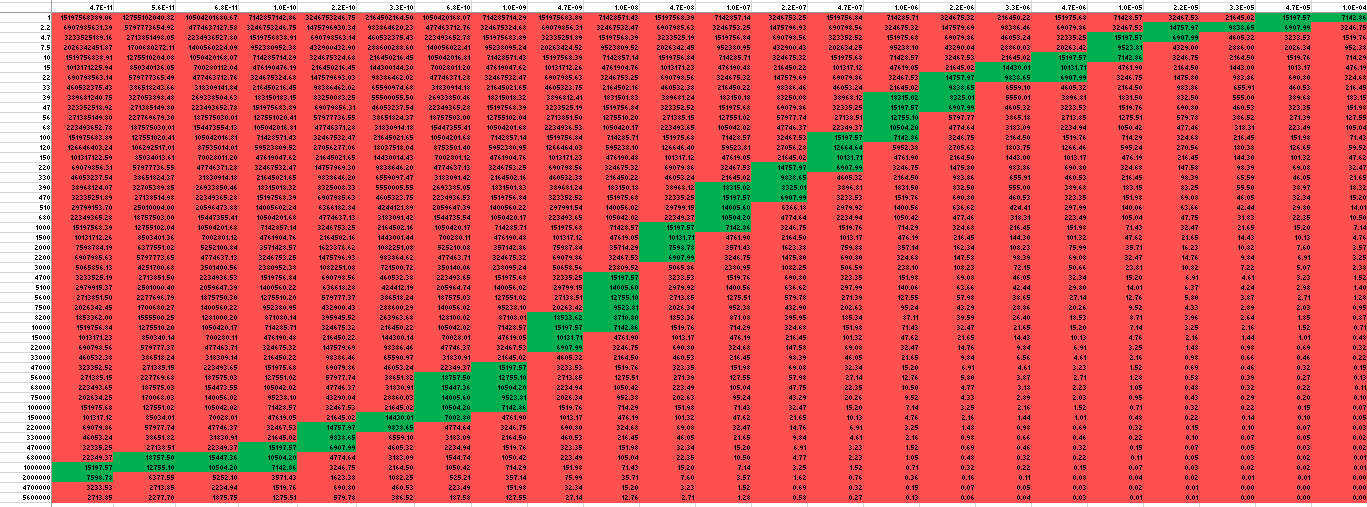
\includegraphics[width=\linewidth]{Figures/6 PCB Design/freq_selection.png}
\end{sidewaysfigure}

There are infinitely many combinations of \code{R} and \code{C} that
will produce any single desired output frequency \code{f}; however, the
set of resistances and capacitances of commonly produced resistors and
capacitors is finite. While multiple components can be combined to
produce more specific resistances and capacitances, doing so would
increase the overall component count for a circuit board that is
constrained to a small physical size. As such, this proof-of-concept
design will focus on producing frequencies attainable with a single
capacitor and resistor pair.

Since each centerpiece transmitter needs to produce four distinct
frequencies, four separate capacitor-resistor pairs are required.
However, since the output frequency can be varied by adjustments to
\emph{either} the capacitance \emph{or} resistance, one of those two
options can be held constant to reduce the overall component count.

To chose which one to hold constant, the output frequencies of all
possible pairings of capacitors and resistors from two cheap Amazon
kits \cite{amazon-capacitors} \cite{amazon-resistors} were calculated
using Equation \ref{eq:555-freq}. The resulting table was then color
coded to highlight the usable frequencies in green (6.67kHz to
20kHz)\footnote{6.67kHz is the lower bound derived in Section
\ref{sec:the-555-timer} and 20kHz the upper limit of the typical
frequency response range discussed in Section
\ref{subsec:frequency-response-range}} while leaving all other unusable
frequencies in red. The result is shown in Figure
\ref{fig:freq-selection} with the various resistances shown on the
vertical axis and the various capacitances along the horizontal axis.

A close observation of the resulting sigmoid shape of usable
frequencies reveals only one location where there are at least four
usable frequencies associated with a fixed resistance (i.e. row of
green cells), compared to ten locations where there are at least four
usable frequencies associated with a fixed capacitance (i.e. column of
green cells). As such, the most practical value to hold constant here
is the capacitance.

One of the locations with a viable fixed capacitance is shown in Figure
\ref{fig:freq-selection-r}. This pairing of a 10nF capacitor with four
resistors with respective resistances of 4.7k$\Omega$, 5.1k$\Omega$,
5.6k$\Omega$, and 7.5k$\Omega$ will be used in the prototype created in
Section \ref{sec:prototype}.

\begin{figure}[h]
    \centering
    \caption{Output Frequencies of Common \code{R} and \code{C} Values}
    \label{fig:freq-selection-r}
    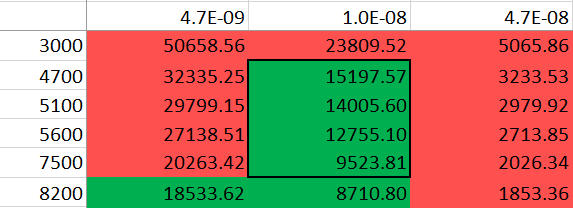
\includegraphics[width=0.8\linewidth]{Figures/6 PCB Design/freq_selection_r.png}
\end{figure}


\section{Prototyping}
\label{sec:prototype}

The key step to produce a proof-of-concept is to put everything
together on a breadboard and turn on the power while recording the
output audio to make sure four distinct tones are produced.

This step begins by gathering all the components from the schematic in
Figure \ref{fig:555_astable_modded} with the specific values of
\code{C}, \code{R1}, \code{R2}, \code{R3}, and \code{R4} shown in
Figure \ref{fig:freq-selection-r}. These components are then placed
onto a physical breadboard in accordance with the schematic's defined
layout. Connecting \code{VDD} and \code{GND} to power then causes the
speaker to produce a tone. With power still connected, the switch can
be moved to put any other resistor in series to change the resulting
tone of the speaker.

The result is shown in Figure \ref{fig:breadboard}. The left section of
the figure shows a spectrogram of the four distinct tones produced by
moving the green wire (representing the rotary switch) through each of
the four resistors on the breadboard in the right section of the figure.

\begin{figure}[h]
    \centering
    \caption{Breadboard Prototype}
    \label{fig:breadboard}
    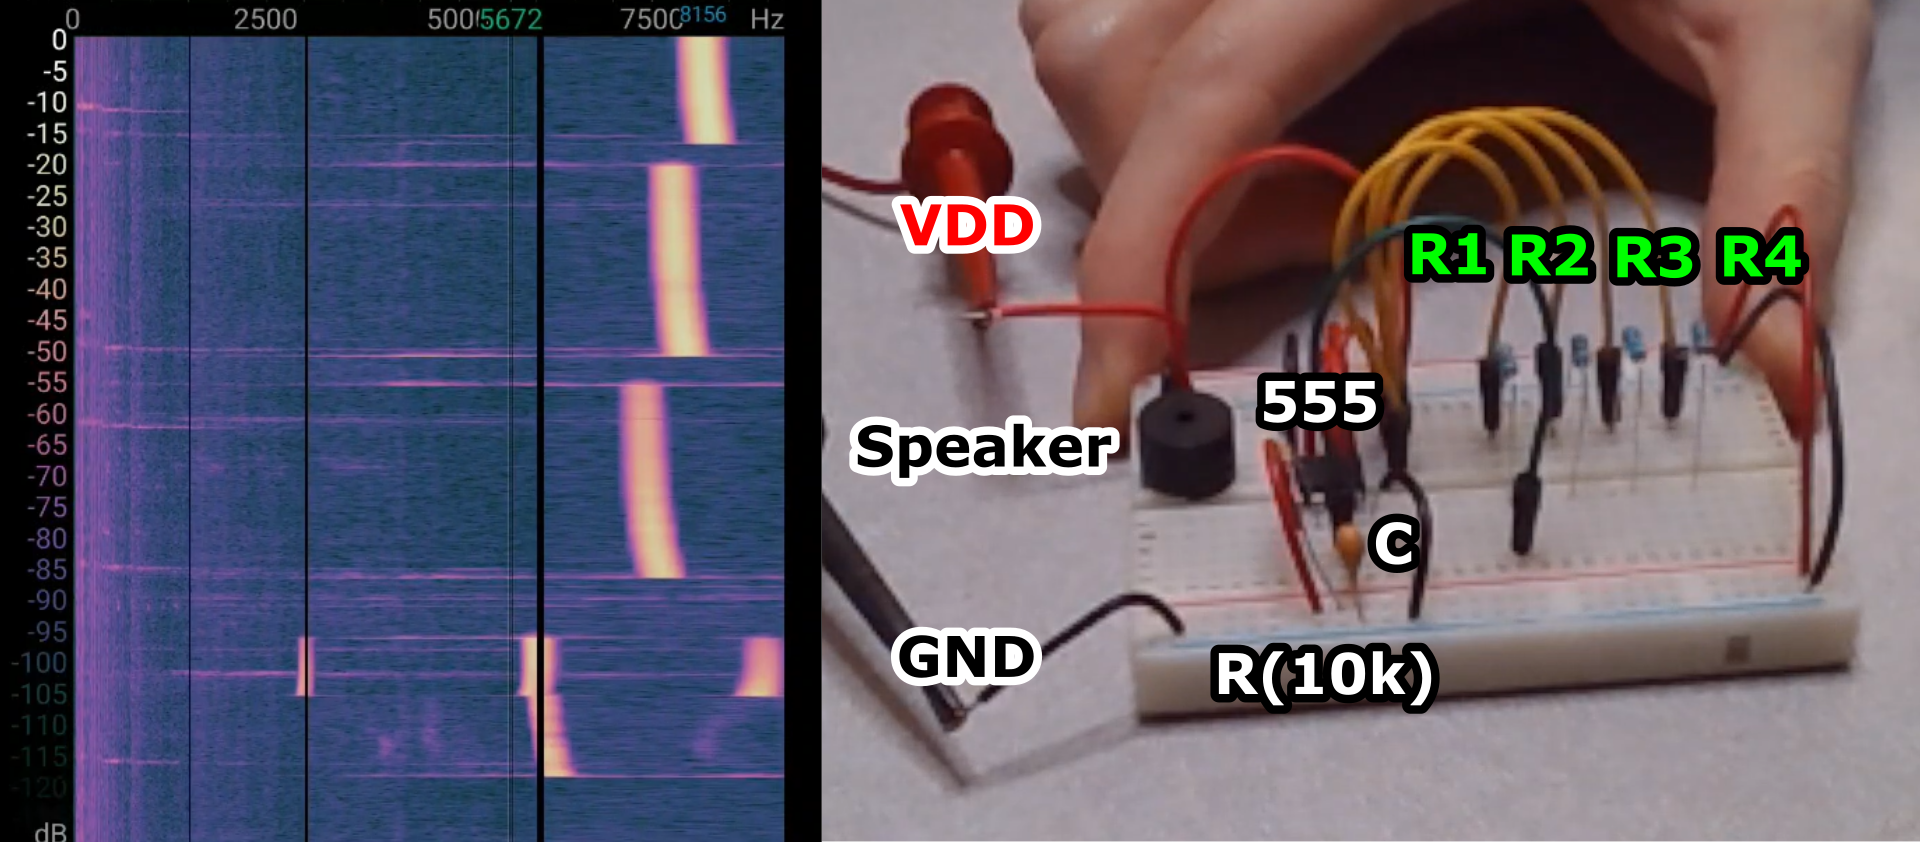
\includegraphics[width=\linewidth]{Figures/6 PCB Design/breadboard_spectrogram.png}
\end{figure}


\section{Miniaturization}
\label{sec:miniaturization}

To further prove the validity of the proof-of-concept finalized in
Section \ref{sec:prototype}, this section will demonstrate that all the
required components can fit within the limited 16mm$^2$ of space inside
a single center cap of a Gans 356 Speedcube.

Meeting this size constraint is best achieved by swapping out the large
through-hole resistors, capacitors, and 555 timer used in the prototype
for smaller surface mount (SMD) components. Additionally, the large
black buzzer can be swapped out for a much thinner piezo buzzer that
can lay on flat on top of a custom-designed replacement centercap.
Finally, the DC power supply can be changed out for a button-cell
battery oriented vertically. An example of the final result could look like Figure \ref{fig:core-placement}.

\begin{figure}[h]
    \centering
    \caption{Transmitter Circuit Inside a Custom Gans 356 Centercap}
    \label{fig:core-placement}
    \begin{subfigure}{.30\textwidth}
        \centering
        \caption{Internal View}
        \label{fig:core-circuit}
        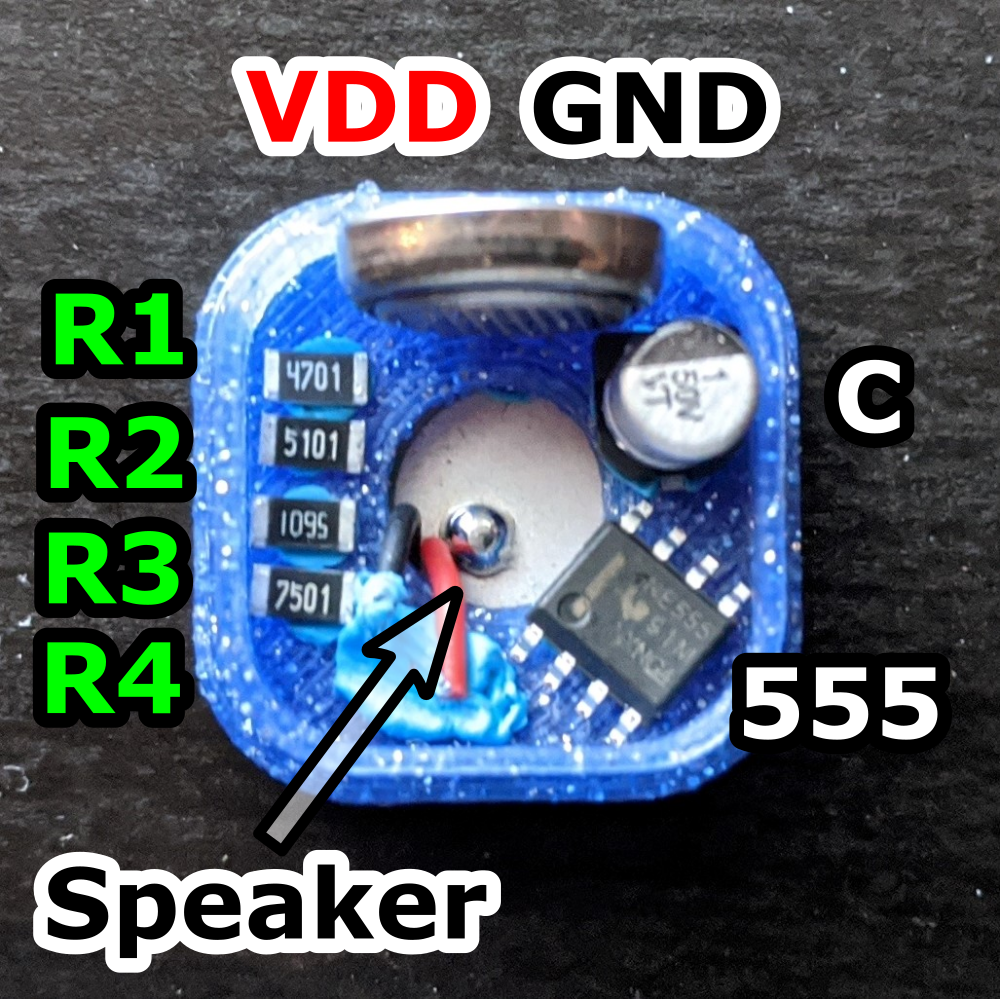
\includegraphics[width=\linewidth]{Figures/6 PCB Design/core_labelled.png}
    \end{subfigure}
    \begin{subfigure}{.30\textwidth}
        \centering
        \caption{Bird's Eye View}
        \label{fig:core-placement-birds-eye}
        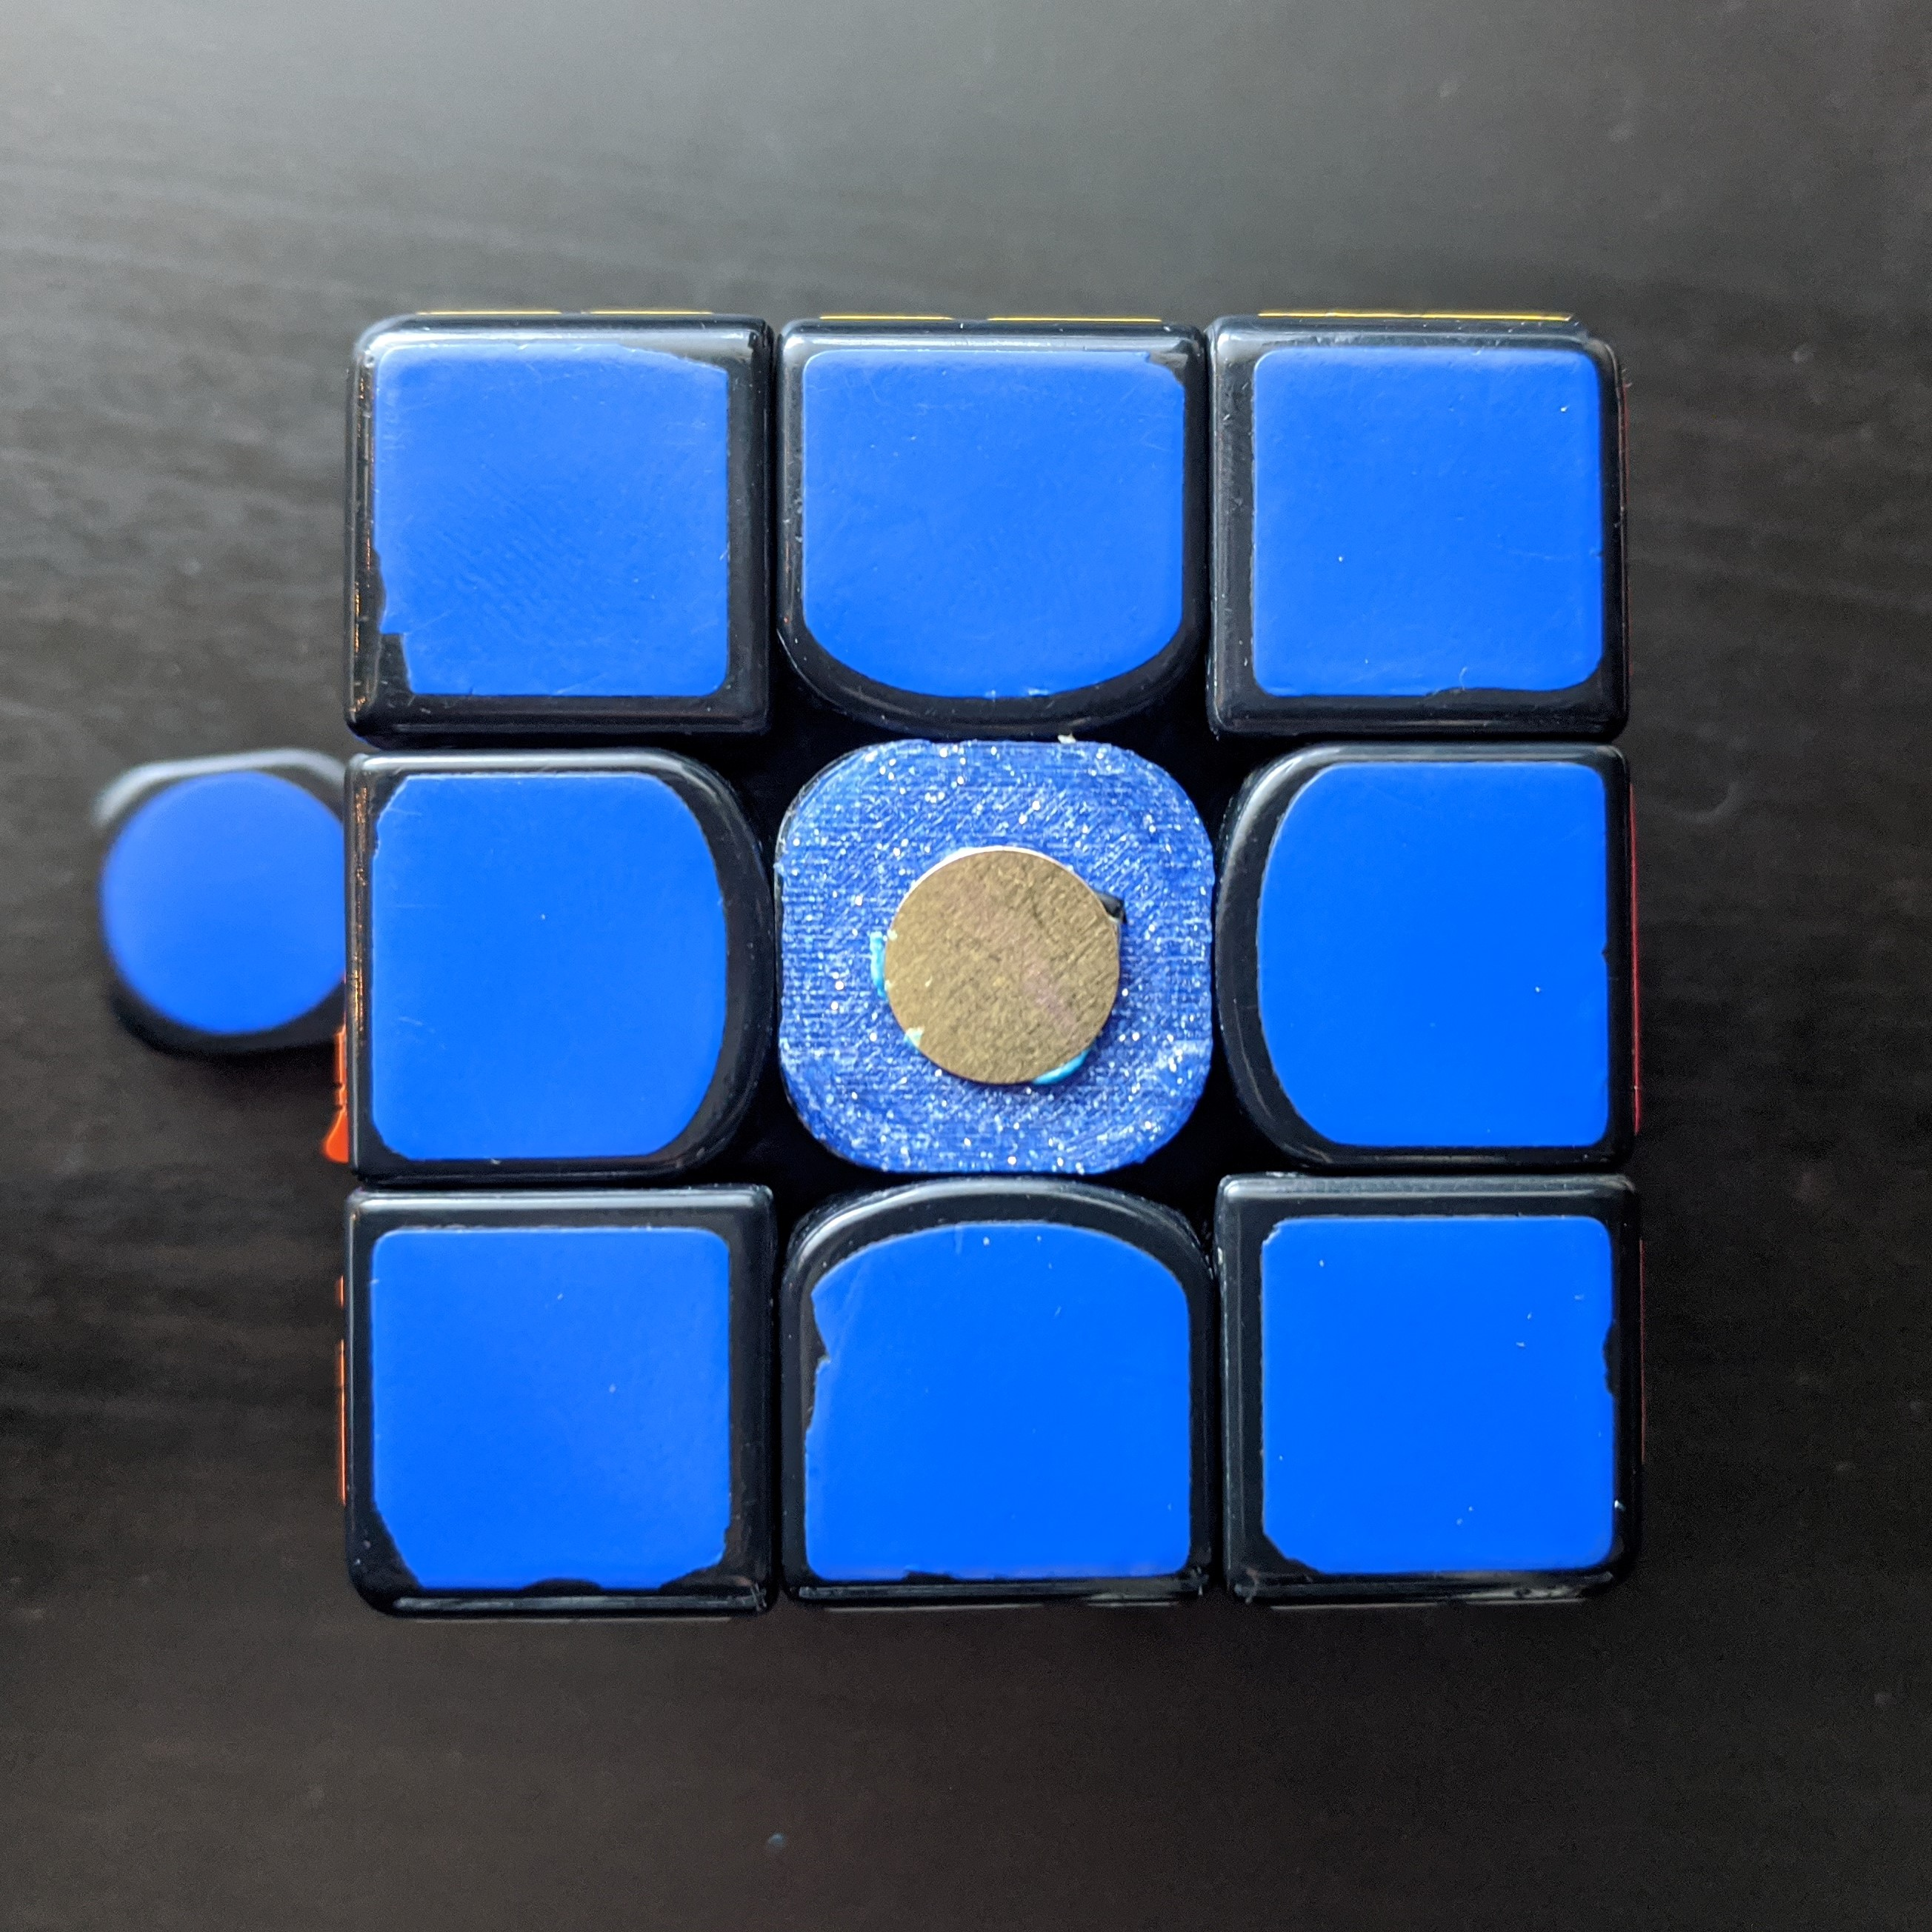
\includegraphics[width=\linewidth]{Figures/6 PCB Design/core_placement_birds_eye_square.jpg}
    \end{subfigure}
    \begin{subfigure}{.30\textwidth}
        \centering
        \caption{Isometric View}
        \label{fig:core-placement-isometric}
        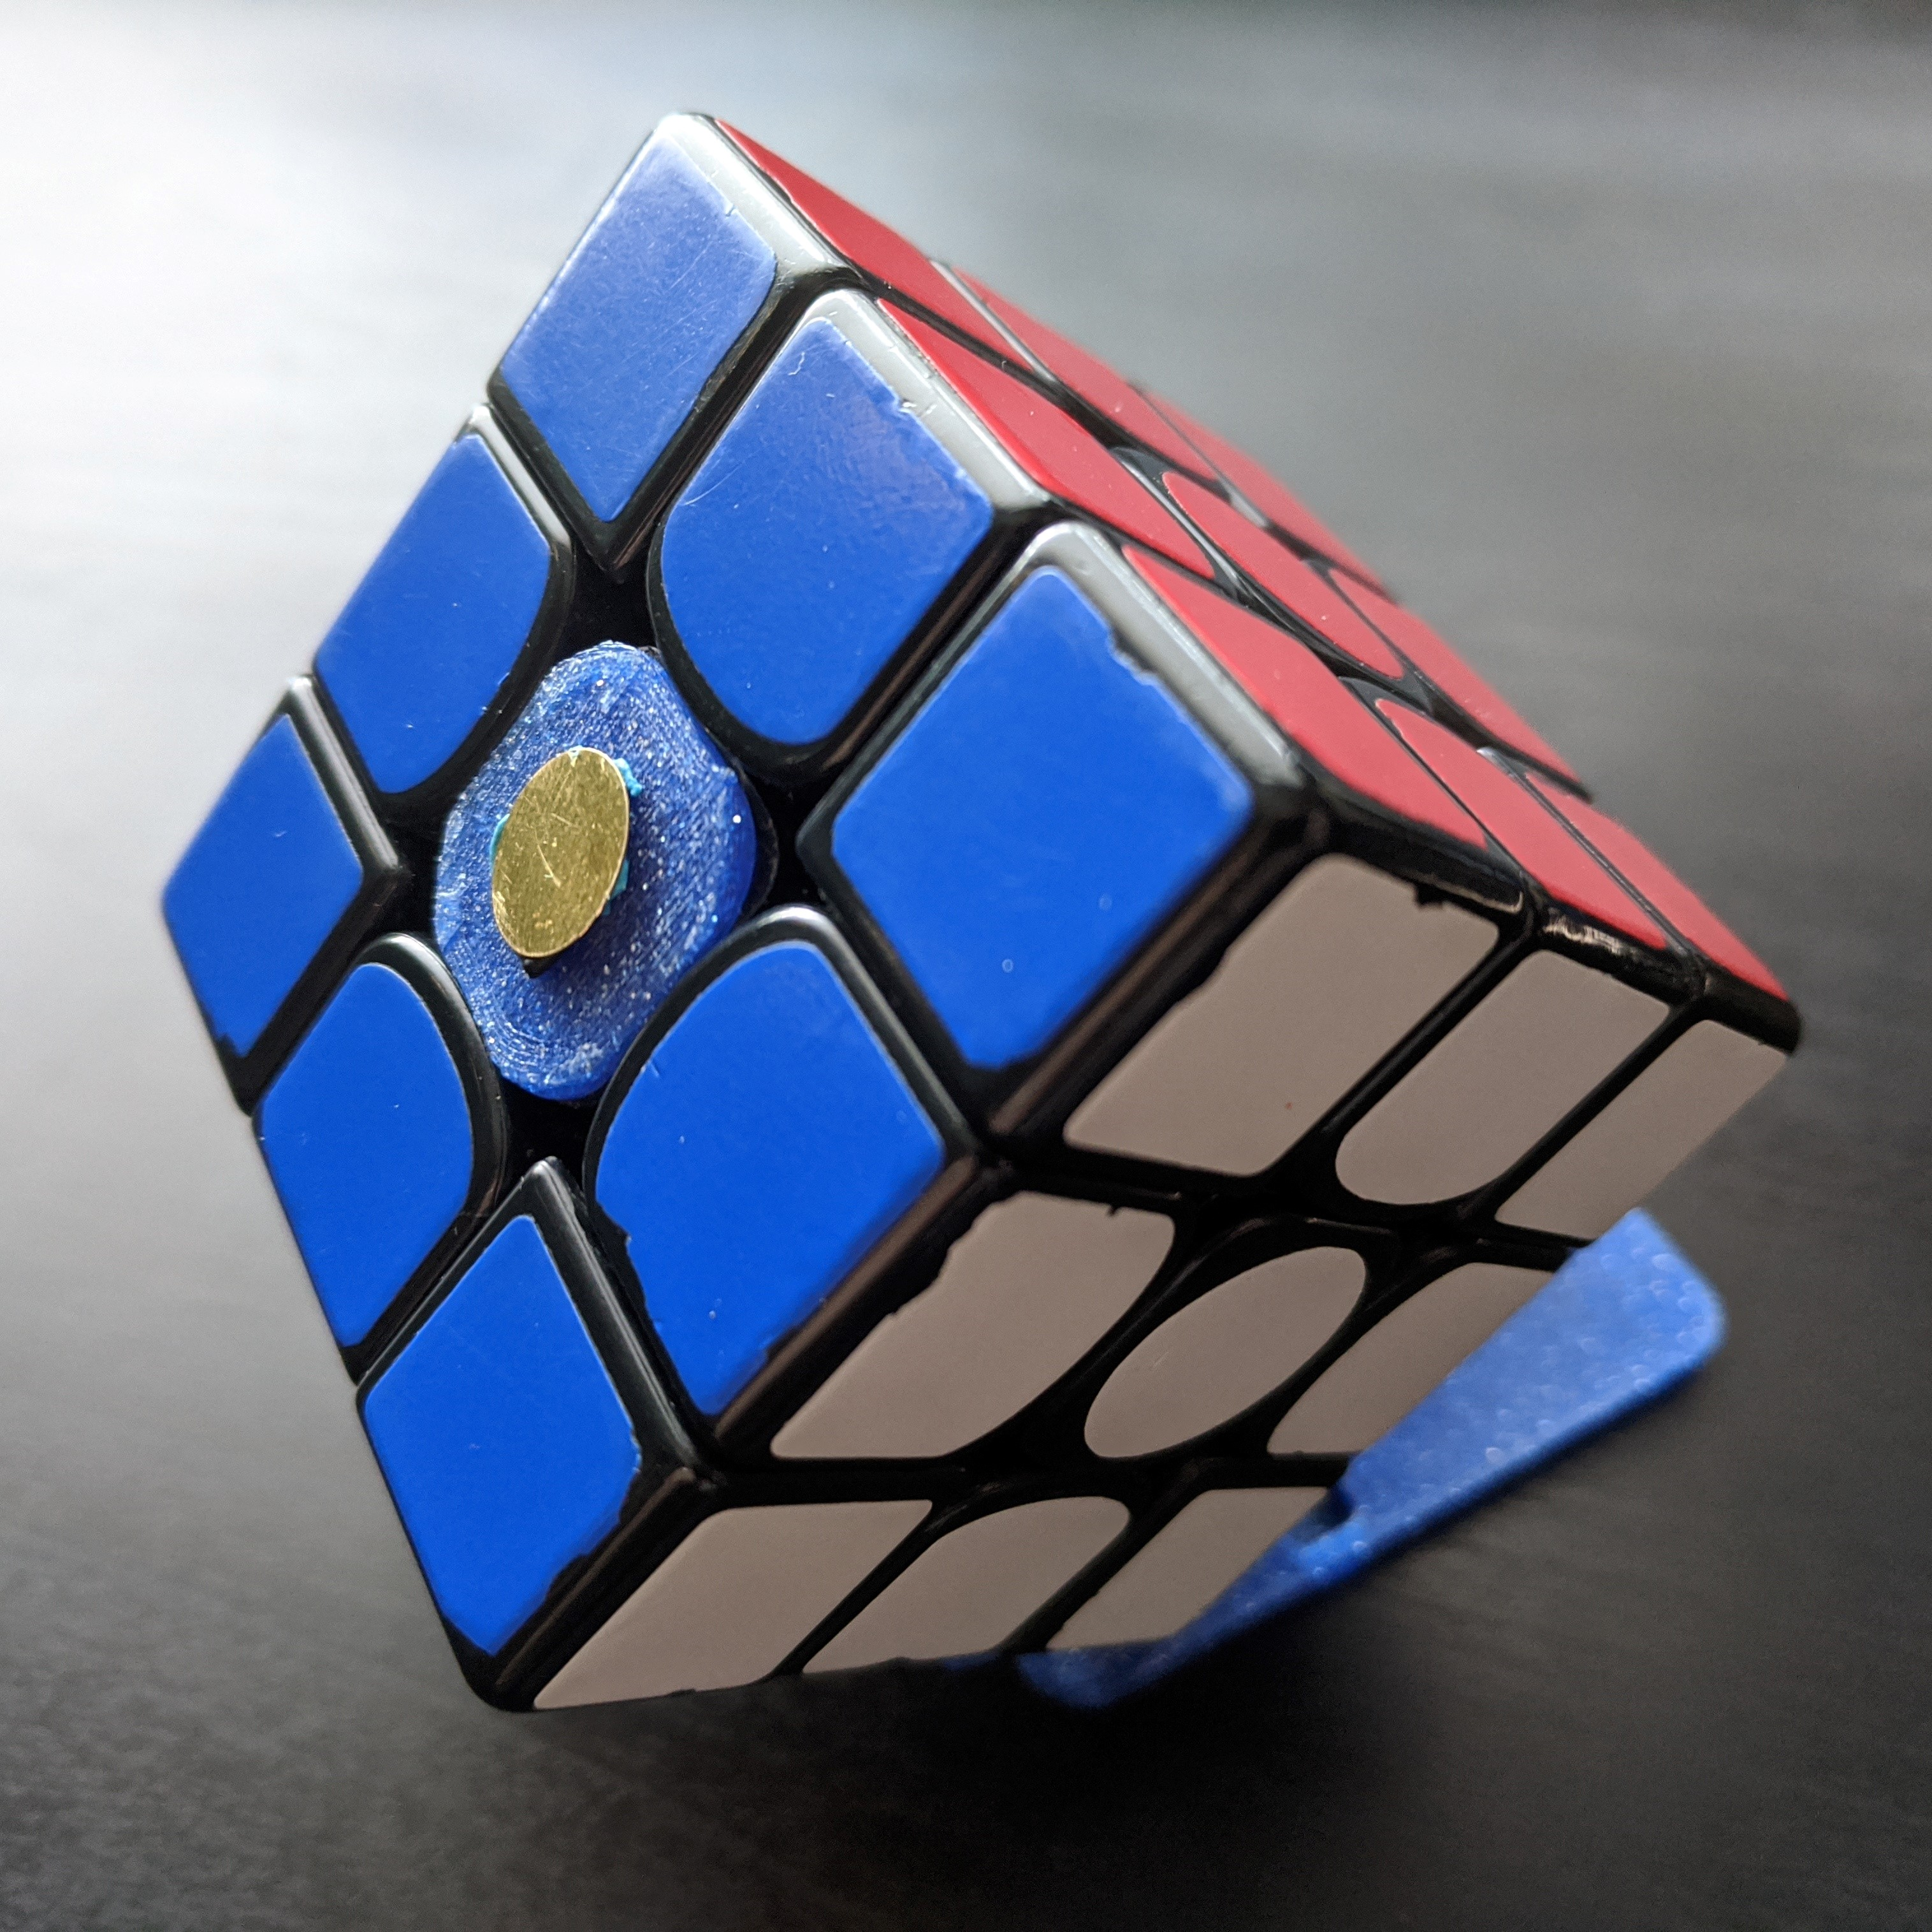
\includegraphics[width=\linewidth]{Figures/6 PCB Design/core_placement_isometric_square.jpg}
    \end{subfigure}
\end{figure}


\section{Summary}

TODO Write this summary
 
\chapter{Evaluation}
\label{Chapter7}

This chapter seeks to measure the effectiveness of the design proposed
in Chapters \ref{Chapter4}, \ref{Chapter5}, and \ref{Chapter6}. To do
so, this chapter will use four key benchmarks derived directly from the
research questions outlined in Section \ref{sec:research-questions}.

The benchmarks are as follows:

\begin{itemize}

    \item \emph{Move Tracking Accuracy}: How accurately can the design
    track the moves performed on the modified speedcube? (Section
    \ref{sec:move-tracking-accuracy})

    \item \emph{Compatibility with Standard Speedcubes}: How
    effectively can the design be deployed in a standard, non-smart
    speedcube without any permanent modifications or reducing the
    cube's performance? (Section
    \ref{sec:compatibility-with-standard-speedcubes})
    
    \item \emph{Move Tracking Granularity}: What other metrics can each 
    design provide (Section \ref{sec:move-tracking-granularity})?
    
    \item \emph{Competition Legality}: To what extent is the design
    compliant with existing competition regulations? (Section
    \ref{sec:competition-legality})
    
\end{itemize}


\section{Move Tracking Accuracy}
\label{sec:move-tracking-accuracy}

For the design to be usable it must be able to track the moves of a
traditional, non-smart speedcube. Furthermore, since untracked moves
render the final move sequence invalid unless manually reviewed and
corrected, it is critical that the design detect moves with high or
perfect accuracy.

While Chapter \ref{Chapter5} demonstrated a perfect detection of a
transmitted move sequence, this section seeks to explore the limits of
the software receiver. To do this, the receiver was subjected to a
battery of tests consisting of running several noisy synthetic audio
sequences (see Section \ref{sec:adding-realistic-noise}) through the
receiver algorithm with a variety of parameters and comparing the
detected move sequence to the one used to generate the audio.

The noisy synthetic audio samples used in this testing were engineered
to represent both the full range of face turns that could be performed
on the cube and the turn speeds of speedcubers that average 12-30
seconds per solve. To that end, the "demo alg" from Figure
\ref{fig:example-alg-audio} which sweeps through every possible
centerpiece state was rendered at 2 TPS and 5 TPS\footnote{Given a that
a typical speedsolver averages 60 moves per solve \cite{pochmann-hume}, 2TPS
corresponds to an average solve time of 30 seconds and 5TPS corresponds
to an average solve time of 12 seconds.} using the code shown in Figure
\ref{fig:code-generate-alg-audio}. Then, those two audio samples were
each augmented with the background noise of a quiet, normal volume, and
noisy speedcube (respectively the Gans 356, Gans X, and QiYi QiMeng
described in Section \ref{subsec:signal-to-noise-ratio}) using the
techniques discussed in Section \ref{sec:adding-realistic-noise} for a
total of 6 audio samples that serve as a basic cross-section of the
most common variations in cubes and turn speeds.

With this representative sample set of audio signals in hand, the
limits of the receiver could be tested. Each test comprised of setting
the three parameters of the receiver to a specific combination of
values (each chosen from a range of values determined emprically),
running all six audio samples through the receiver, then comparing the
detected move sequence with the actual move sequence for a percent
similarity calculation. The standard deviation threshold parameter
\code{stdv\_pct} (Section \ref{subsec:fine-tuning-threshold}) varied
through from 0.25 to 3 in increments of 0.25 for a total of 12 values.
The minimum threshold parameter \code{min\_thresh} (Section
\ref{subsec:fine-tuning-threshold}) varied from 50 to 550 in increments
of 50 for a total of 6 values. The window size parameter
\code{window\_size} (Section
\ref{subsec:ignoring-noise-when-extracting-move-sequences}) varied from
1 to 10 time steps in increments of 1 for a total of 10 values. In
total, the 12 standard deviation thresholds, 6 minimum thresholds, 10
window sizes, 2 turn speeds, and 3 cubes yielded 4,320 unique
combinations with which to test the receiver algorithm.

The insights gained from analyzing the resulting data are discussed in
the following subsections. Section
\ref{subsec:influence-cube-noisiness} explores the influence of cube
noisiness on detection accuracy. Section
\ref{subsec:influence-stdv-threshold} does the same for the standard
deviation threshold. Section \ref{subsec:influence-alt-min} covers the
minimum threshold. And Section \ref{subsec:influence-window-size}
reviews the window size. The turn speed factor is discussed in all
subsections as an additional angle for understanding each factor's
unique influence on detection accuracy.

\subsection{Influence of Cube Noisiness}
\label{subsec:influence-cube-noisiness}

The three cubes used for this analysis - the Gans 356, Gans XS, and
QiYi Qimeng - respectively represent quiet, normal, and loud speedcubes
(see Section \ref{subsec:signal-to-noise-ratio}). The louder speedcubes
were expected to cause more difficulties for decoding the transmitted
move sequence since they create more noise that may conflict with the
audible signal. Since all cubes produced more noise when turned at a
higher speed and there is less time for detection to complete, the
simulated turn speeds were also expected to experience inferior
performance during move sequence detection.

\begin{figure}
\caption{Perfect Detections by Cube}
\label{fig:perfect-detections-by-cube}
\begin{subfigure}{\textwidth}
    \centering
    \caption{Total number of perfect detections \\ (Aggregate of Figures \ref{fig:perfect-detections-by-cube-2tps} and \ref{fig:perfect-detections-by-cube-5tps})}
    \label{fig:perfect-detections-by-cube-total}
    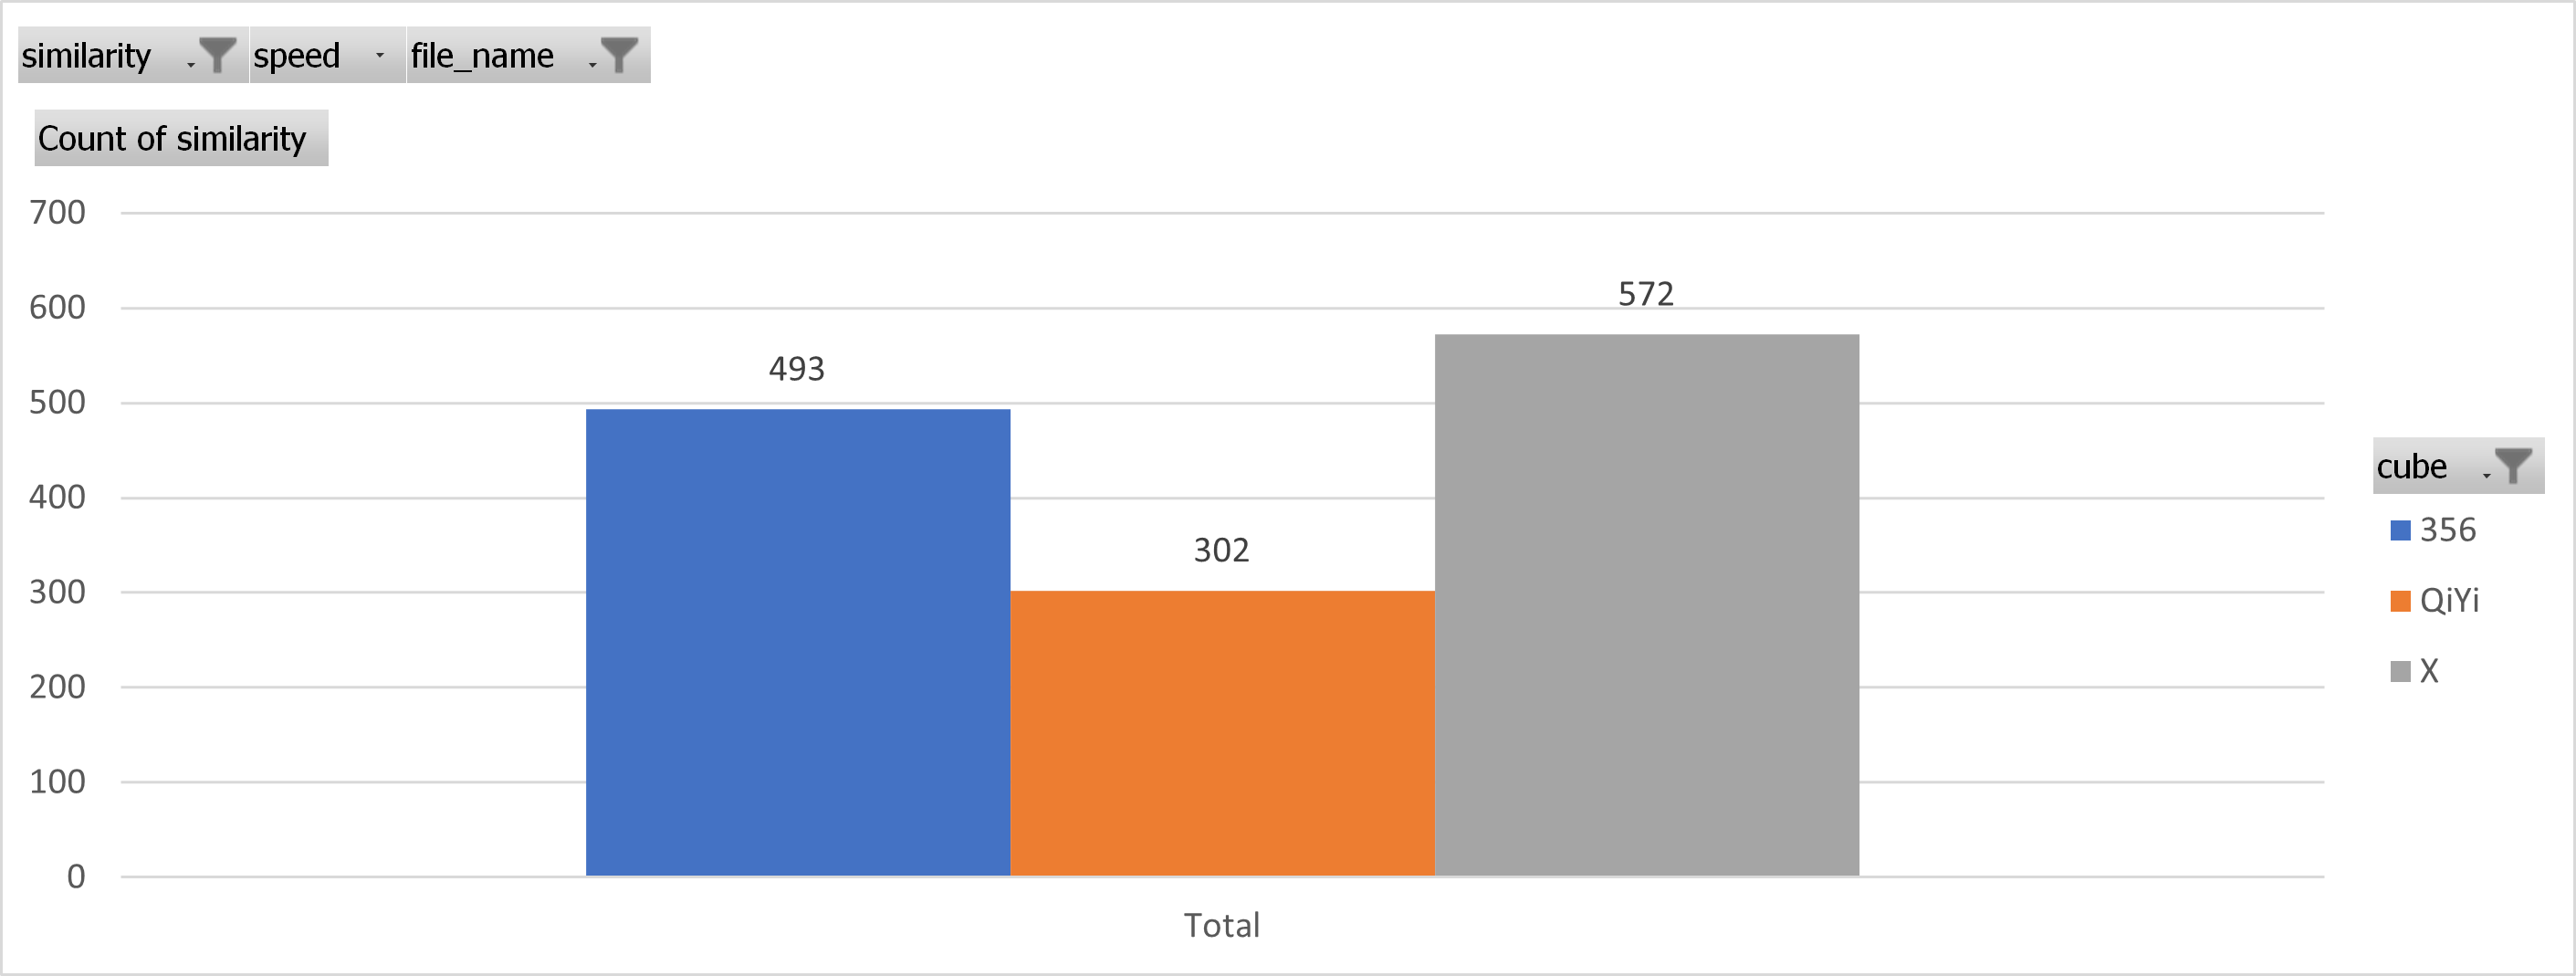
\includegraphics[width=\linewidth]{Figures/7 Evaluation/perfect_detections_by_cube.png}
    \vspace*{.1mm}
\end{subfigure}\\
\begin{subfigure}{\textwidth}
    \centering
    \caption{Total number of perfect detections at 2TPS}
    \label{fig:perfect-detections-by-cube-2tps}
    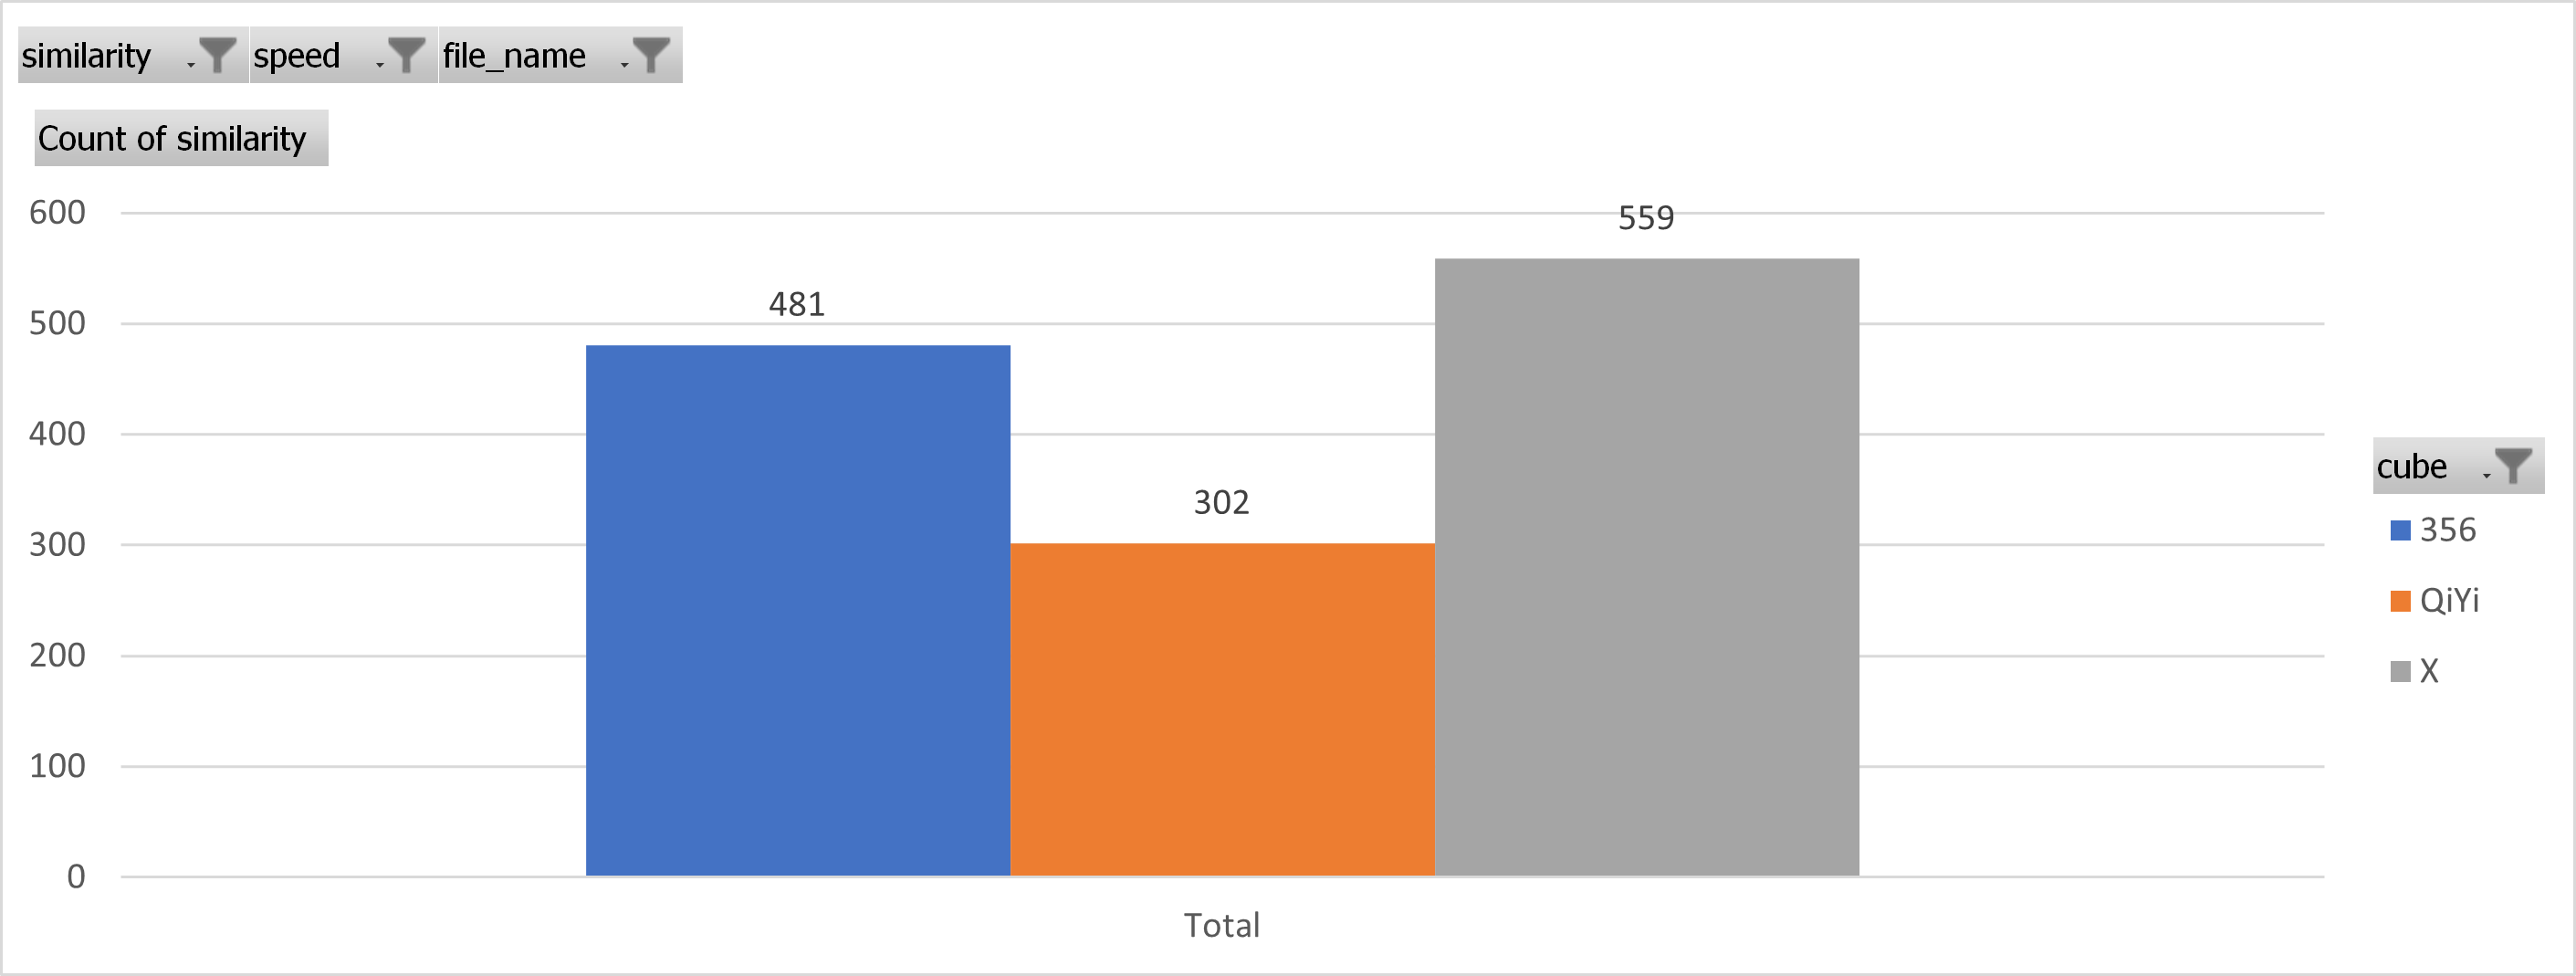
\includegraphics[width=\linewidth]{Figures/7 Evaluation/perfect_detections_by_cube_2tps.png}
    \vspace*{.1mm}
\end{subfigure}\\
\begin{subfigure}{\textwidth}
    \centering
    \caption{Total number of perfect detections at 5TPS}
    \label{fig:perfect-detections-by-cube-5tps}
    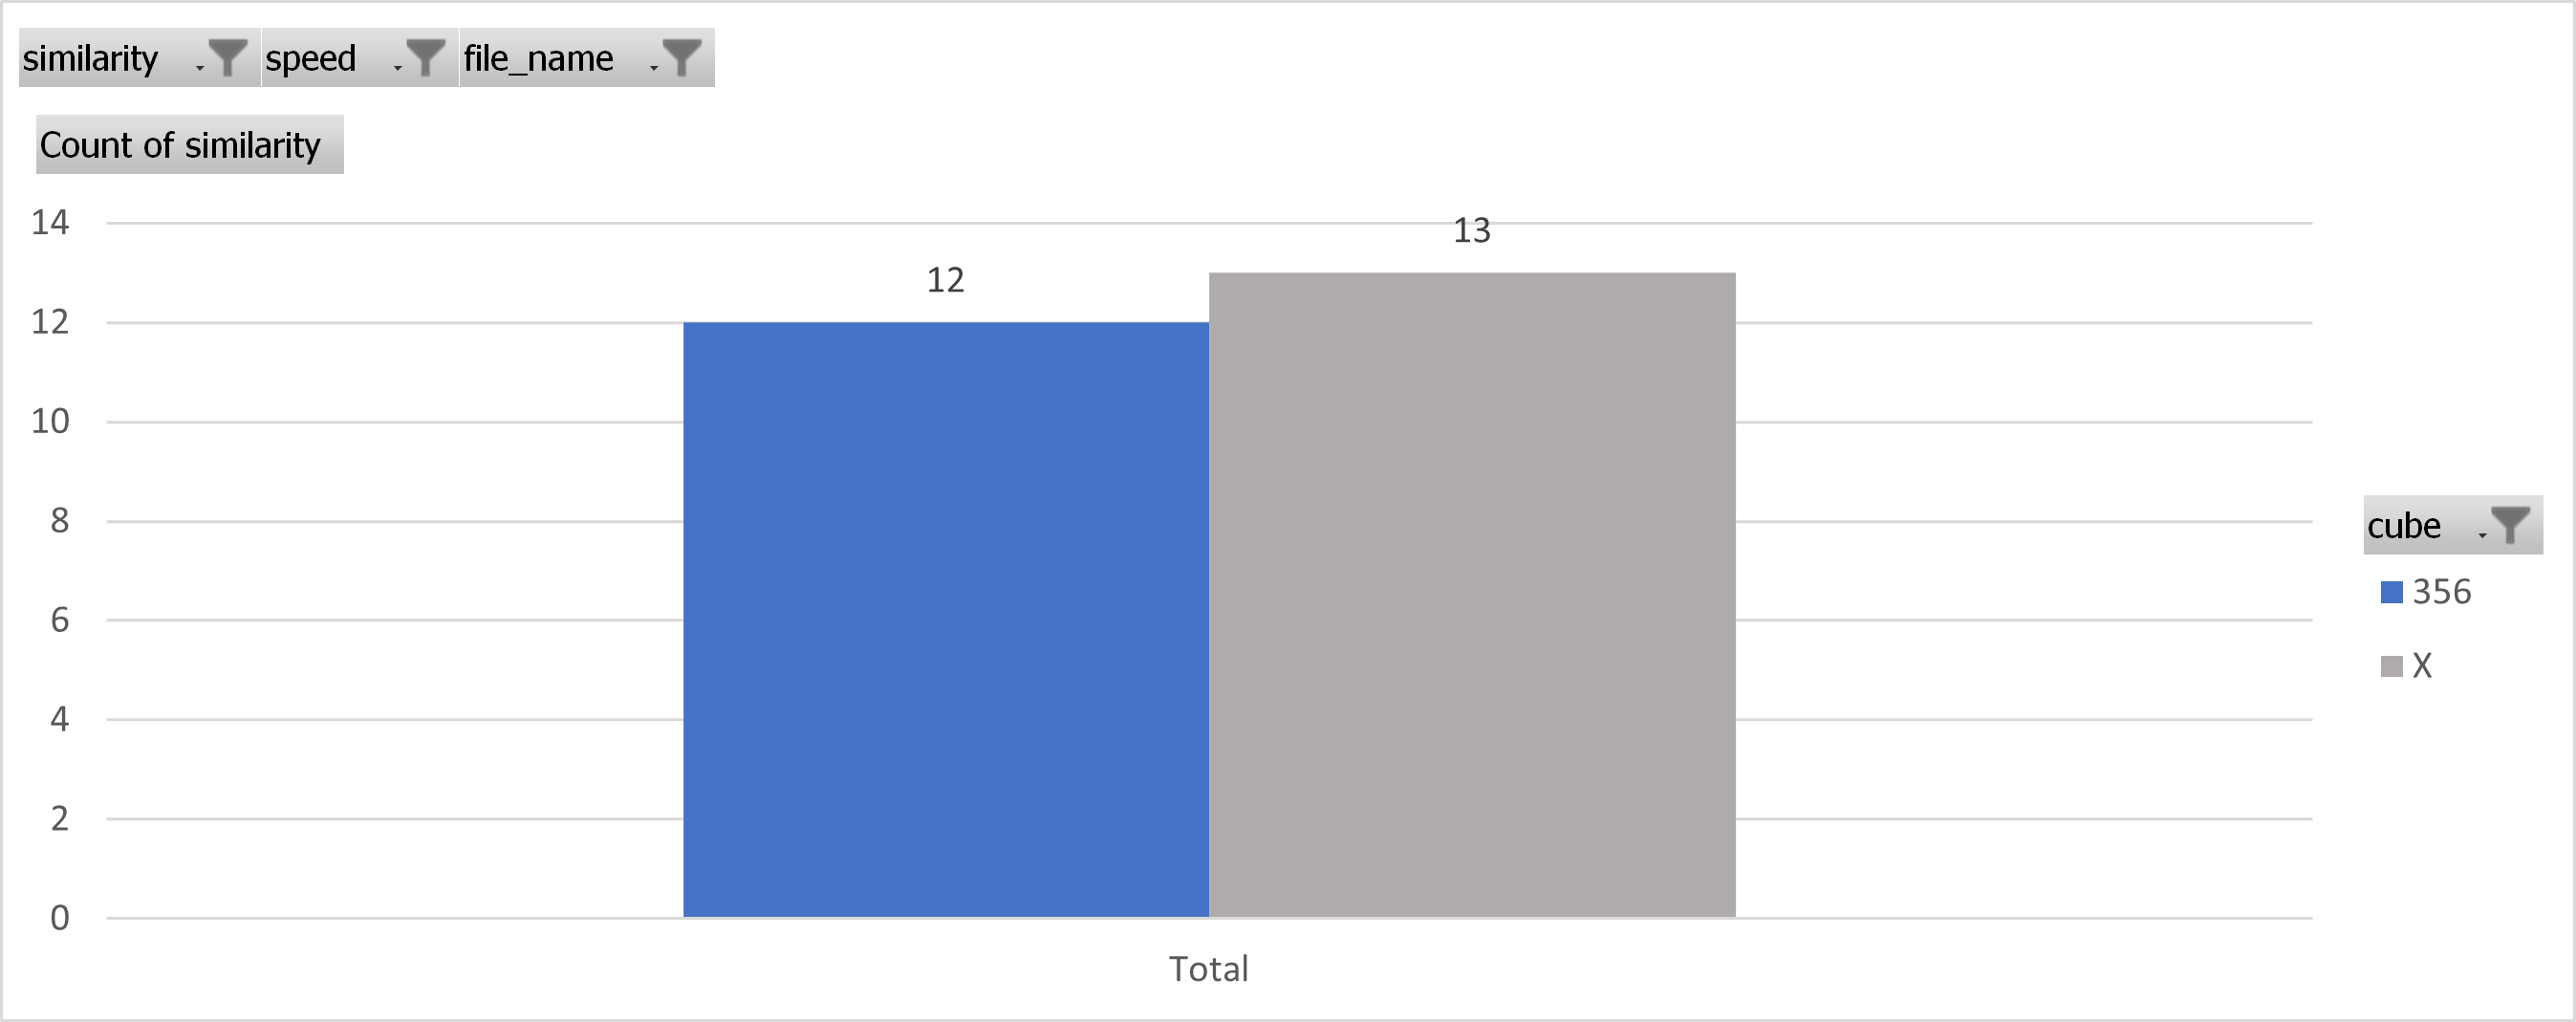
\includegraphics[width=\linewidth]{Figures/7 Evaluation/perfect_detections_by_cube_5tps.png}
    \vspace*{.1mm}
\end{subfigure}\\
\end{figure}

Figure \ref{fig:perfect-detections-by-cube} shows the total number of
perfect move sequence decodings broken down by cube type and simulated
turn speed. As expected, there were far fewer perfect detections at the
higher simulated turn speed compared to the lower simulated turn speed,
with the loud QiYi even failing to register a single perfect detection
at the higher turn speed. However, it was the normal noise Gans XS, not
the quiet Gans 356 that achieved the most perfect detections. This is a
peculiar result since Figure \ref{fig:signal-to-noise-ratio} shows that
the Gans XS is louder across a wider frequency spectrum than the Gans
356.

\subsection{Influence of the Standard Deviation Threshold}
\label{subsec:influence-stdv-threshold}

The standard deviation threshold was one piece of the threshold
calculation used to filter out background noise (see Section
\ref{subsec:fine-tuning-threshold}). Since frequency peaks tend to be
statistical outliers, higher thresholds were expected to filter out
more background noise, thus providing higher detection accuracy, so
long as the thresholds were not so high as to exclude the peaks
themselves.

Figure \ref{fig:influence-stdv-threshold-perfect} shows the total number of
perfect move sequence decodings broken down by the standard deviation
threshold. Contrary to the expectations, the slightly sinusoidal results show that lower thresholds generally corresponded to slightly better chances of achieving a perfect detection than higher thresholds.

However, Figures \ref{fig:influence-stdv-threshold-average-2tps} and
\ref{fig:influence-stdv-threshold-average-5tps} suggest that, overall,
a higher standard deviation threshold typically corresponds to a higher
average detection accuracy across all variations of the other parameters in
this experiment. Of particular interest is the continuous improvement
in detection accuracy experienced by the noisy QiYi Qimeng as the
standard deviation threshold increased, particularly for the 5TPS audio
sequences where it achieved a higher average accuracy than either of
its less noisy counterparts.

\begin{figure}
    \caption{Influence of Standard Deviation Threshold on Accuracy}
    \label{fig:influence-stdv-threshold}
    \begin{subfigure}{\textwidth}
        \centering
        \caption{Perfect Detections by Standard Deviation Threshold}
        \label{fig:influence-stdv-threshold-perfect}
        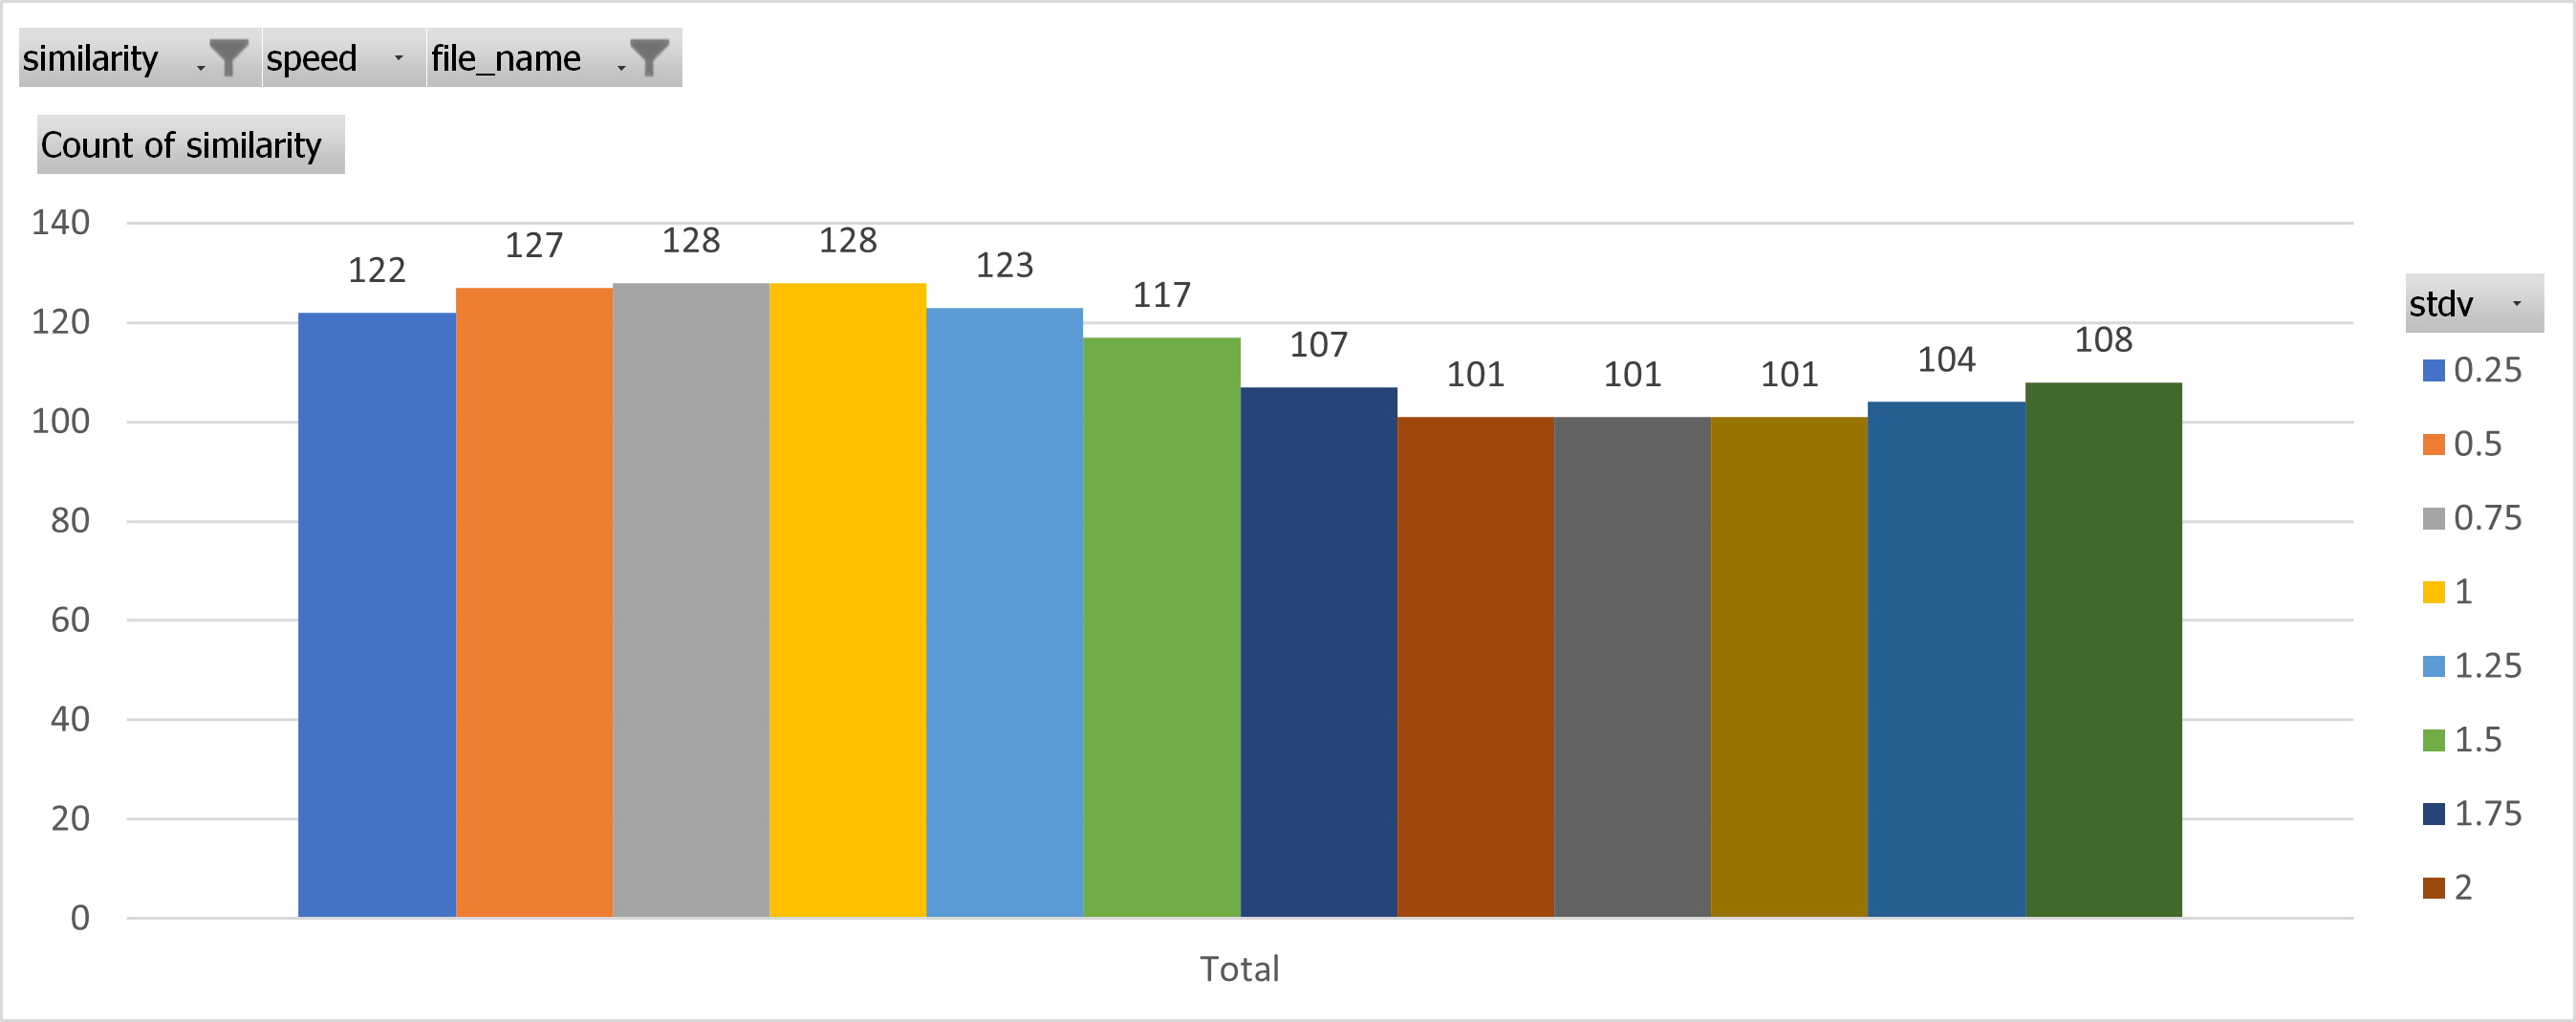
\includegraphics[width=\linewidth]{Figures/7 Evaluation/perfect_detections_by_stdv.png}
        \vspace*{.1mm}
    \end{subfigure}\\
    \begin{subfigure}{\textwidth}
        \centering
        \caption{Average Accuracy by Standard Deviation Threshold at 2 TPS}
        \label{fig:influence-stdv-threshold-average-2tps}
        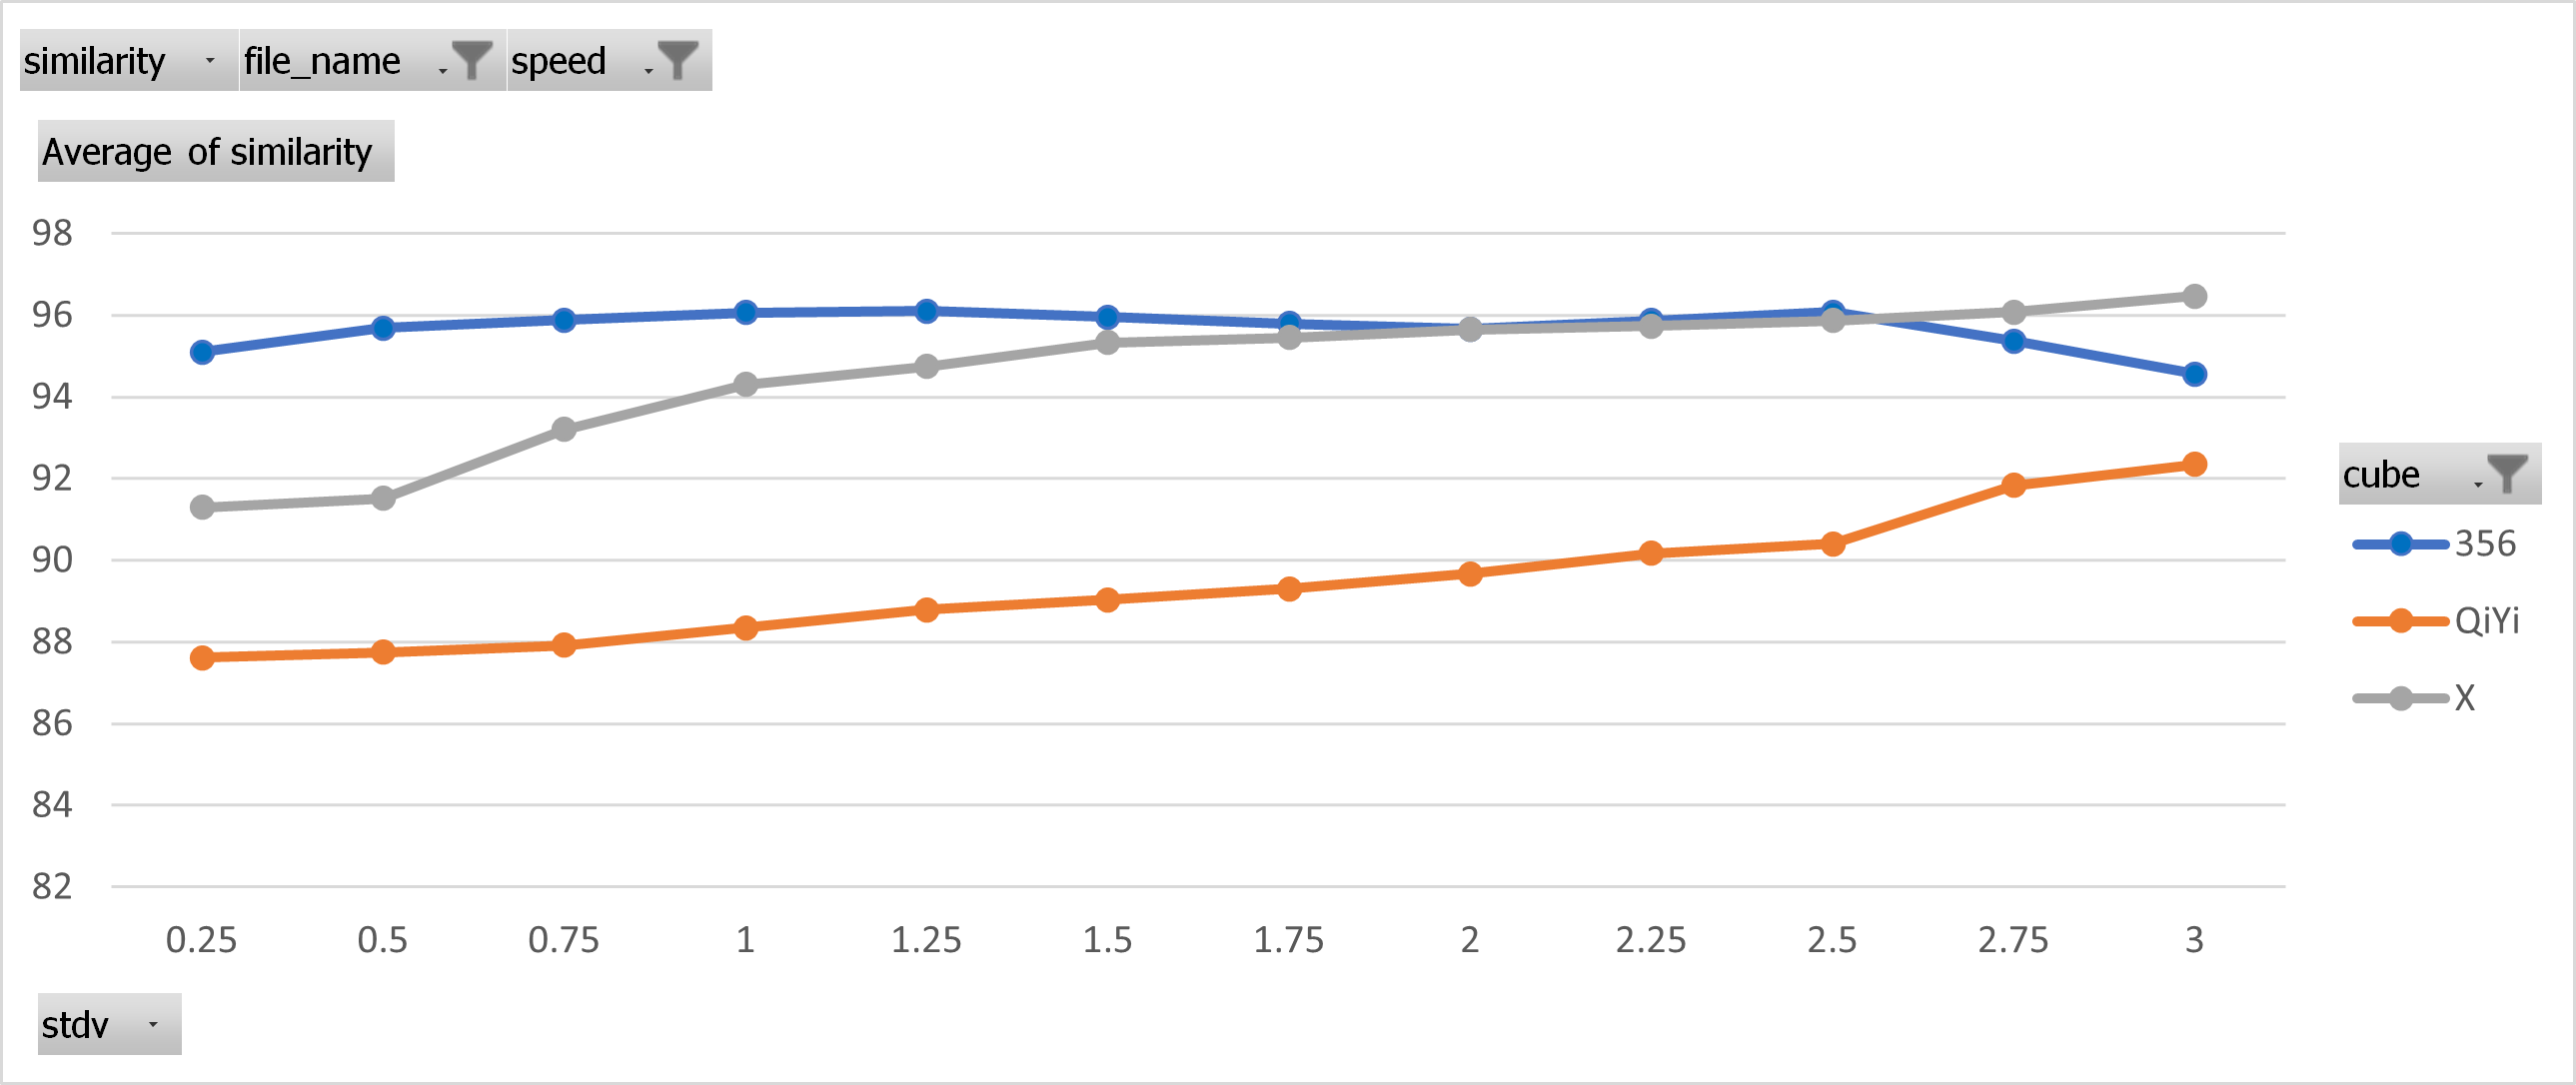
\includegraphics[width=\linewidth]{Figures/7 Evaluation/similarity_by_stdv_2tps.png}
        \vspace*{.1mm}
    \end{subfigure}\\
    \begin{subfigure}{\textwidth}
        \centering
        \caption{Average Accuracy by Standard Deviation Threshold at 5 TPS}
        \label{fig:influence-stdv-threshold-average-5tps}
        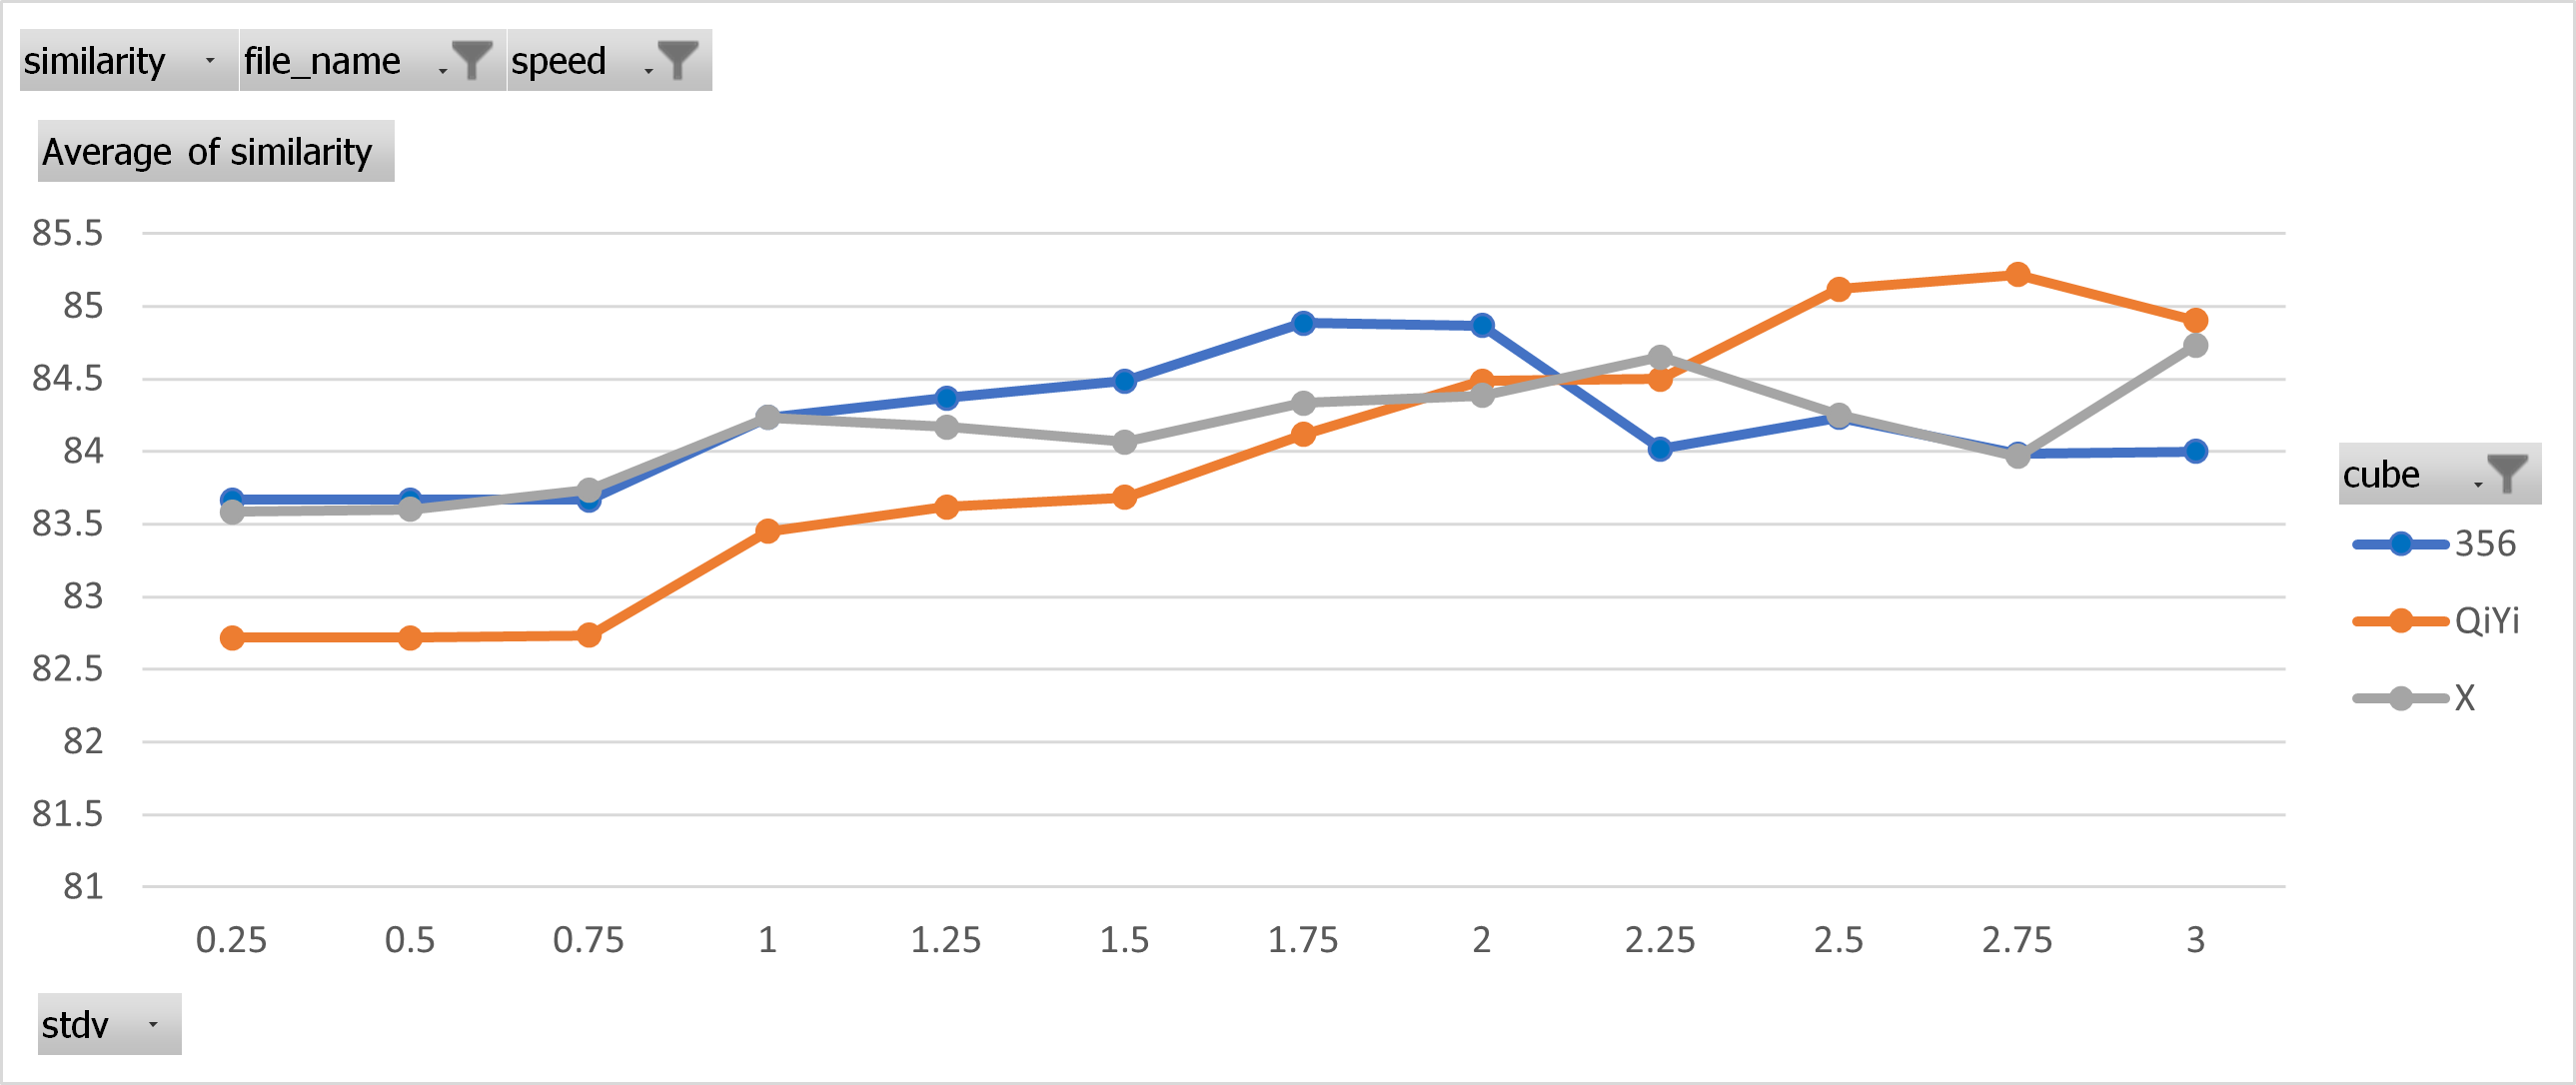
\includegraphics[width=\linewidth]{Figures/7 Evaluation/similarity_by_stdv_5tps.png}
        \vspace*{.1mm}
    \end{subfigure}\\
\end{figure}

\subsection{Influence of Minimum Threshold}
\label{subsec:influence-alt-min}

The minimum threshold was the second component in the threshold
calculation discussed in Section \ref{subsec:fine-tuning-threshold},
used primarily to filter out background noise during the quiet signal
period between face turns. Similar to the standard deviation threshold,
higher minimum thresholds were expected to yield higher detection
accuracies, particularly for noisy cubes.

Interestingly, the minimum threshold performed similarly to the
standard deviation threshold in regard to its correlation with perfect
move sequence detections (Figure
\ref{fig:perfect-detections-by-alt-min-total}). However, in contrast to
the standard deviation threshold, the minimum threshold corresponded to
far less variation in the average accuracy, though accuracy did trend
upwards as the minimum threshold increased.

\begin{figure}
    \caption{Perfect Detections by Minimum Threshold}
    \label{fig:influence-alt-min}
    \begin{subfigure}{\textwidth}
        \centering
        \caption{Total number of perfect detections}
        \label{fig:perfect-detections-by-alt-min-total}
        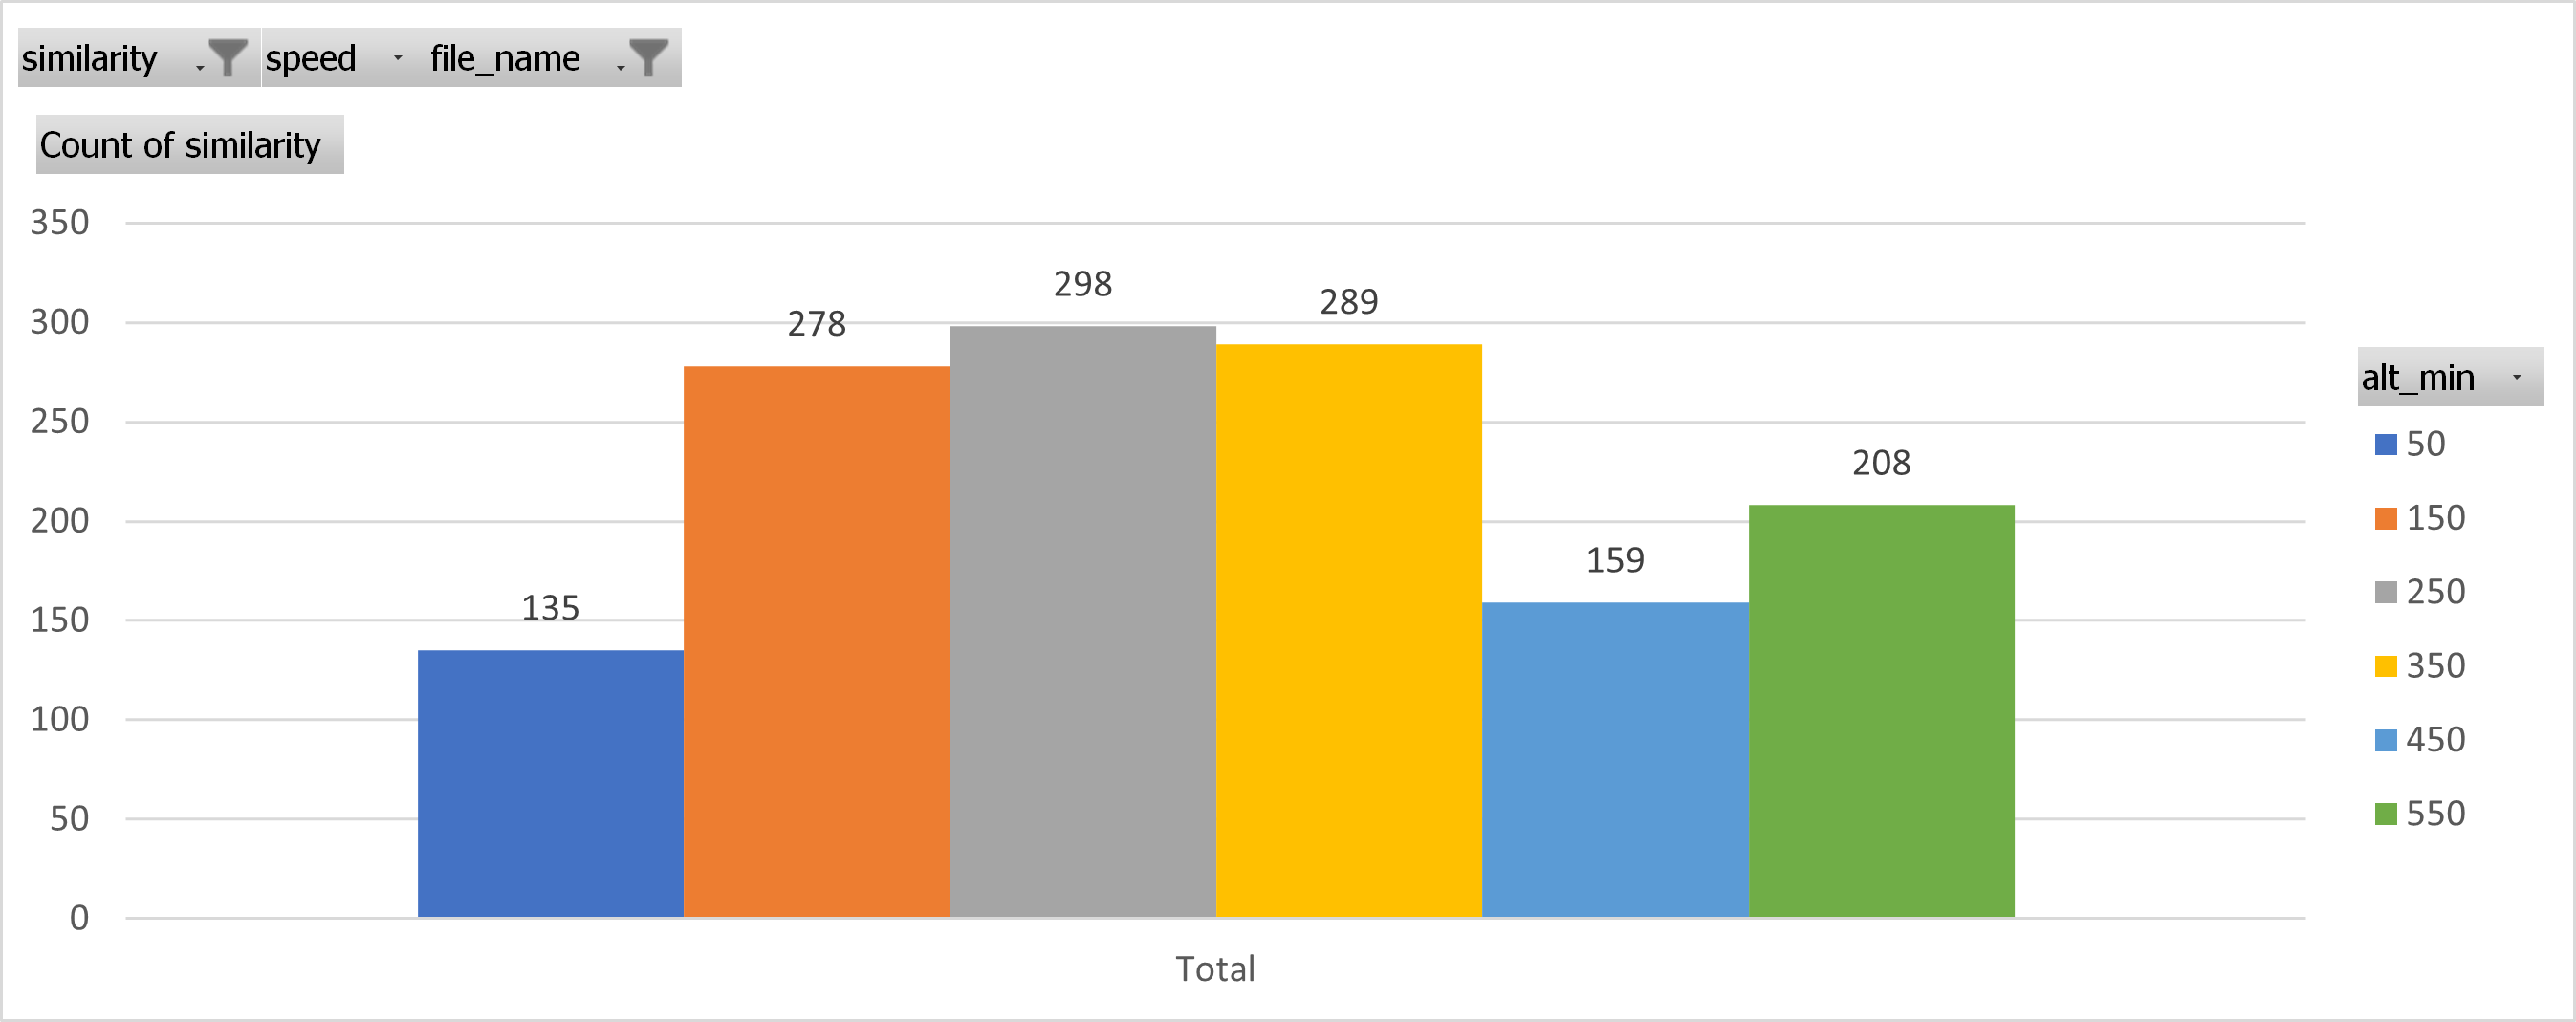
\includegraphics[width=\linewidth]{Figures/7 Evaluation/perfect_detections_by_alt_min.png}
        \vspace*{.1mm}
    \end{subfigure}\\
    \begin{subfigure}{\textwidth}
        \centering
        \caption{Average Accuracy by Minimum Threshold at 2 TPS}
        \label{fig:influence-alt-min-average-2tps}
        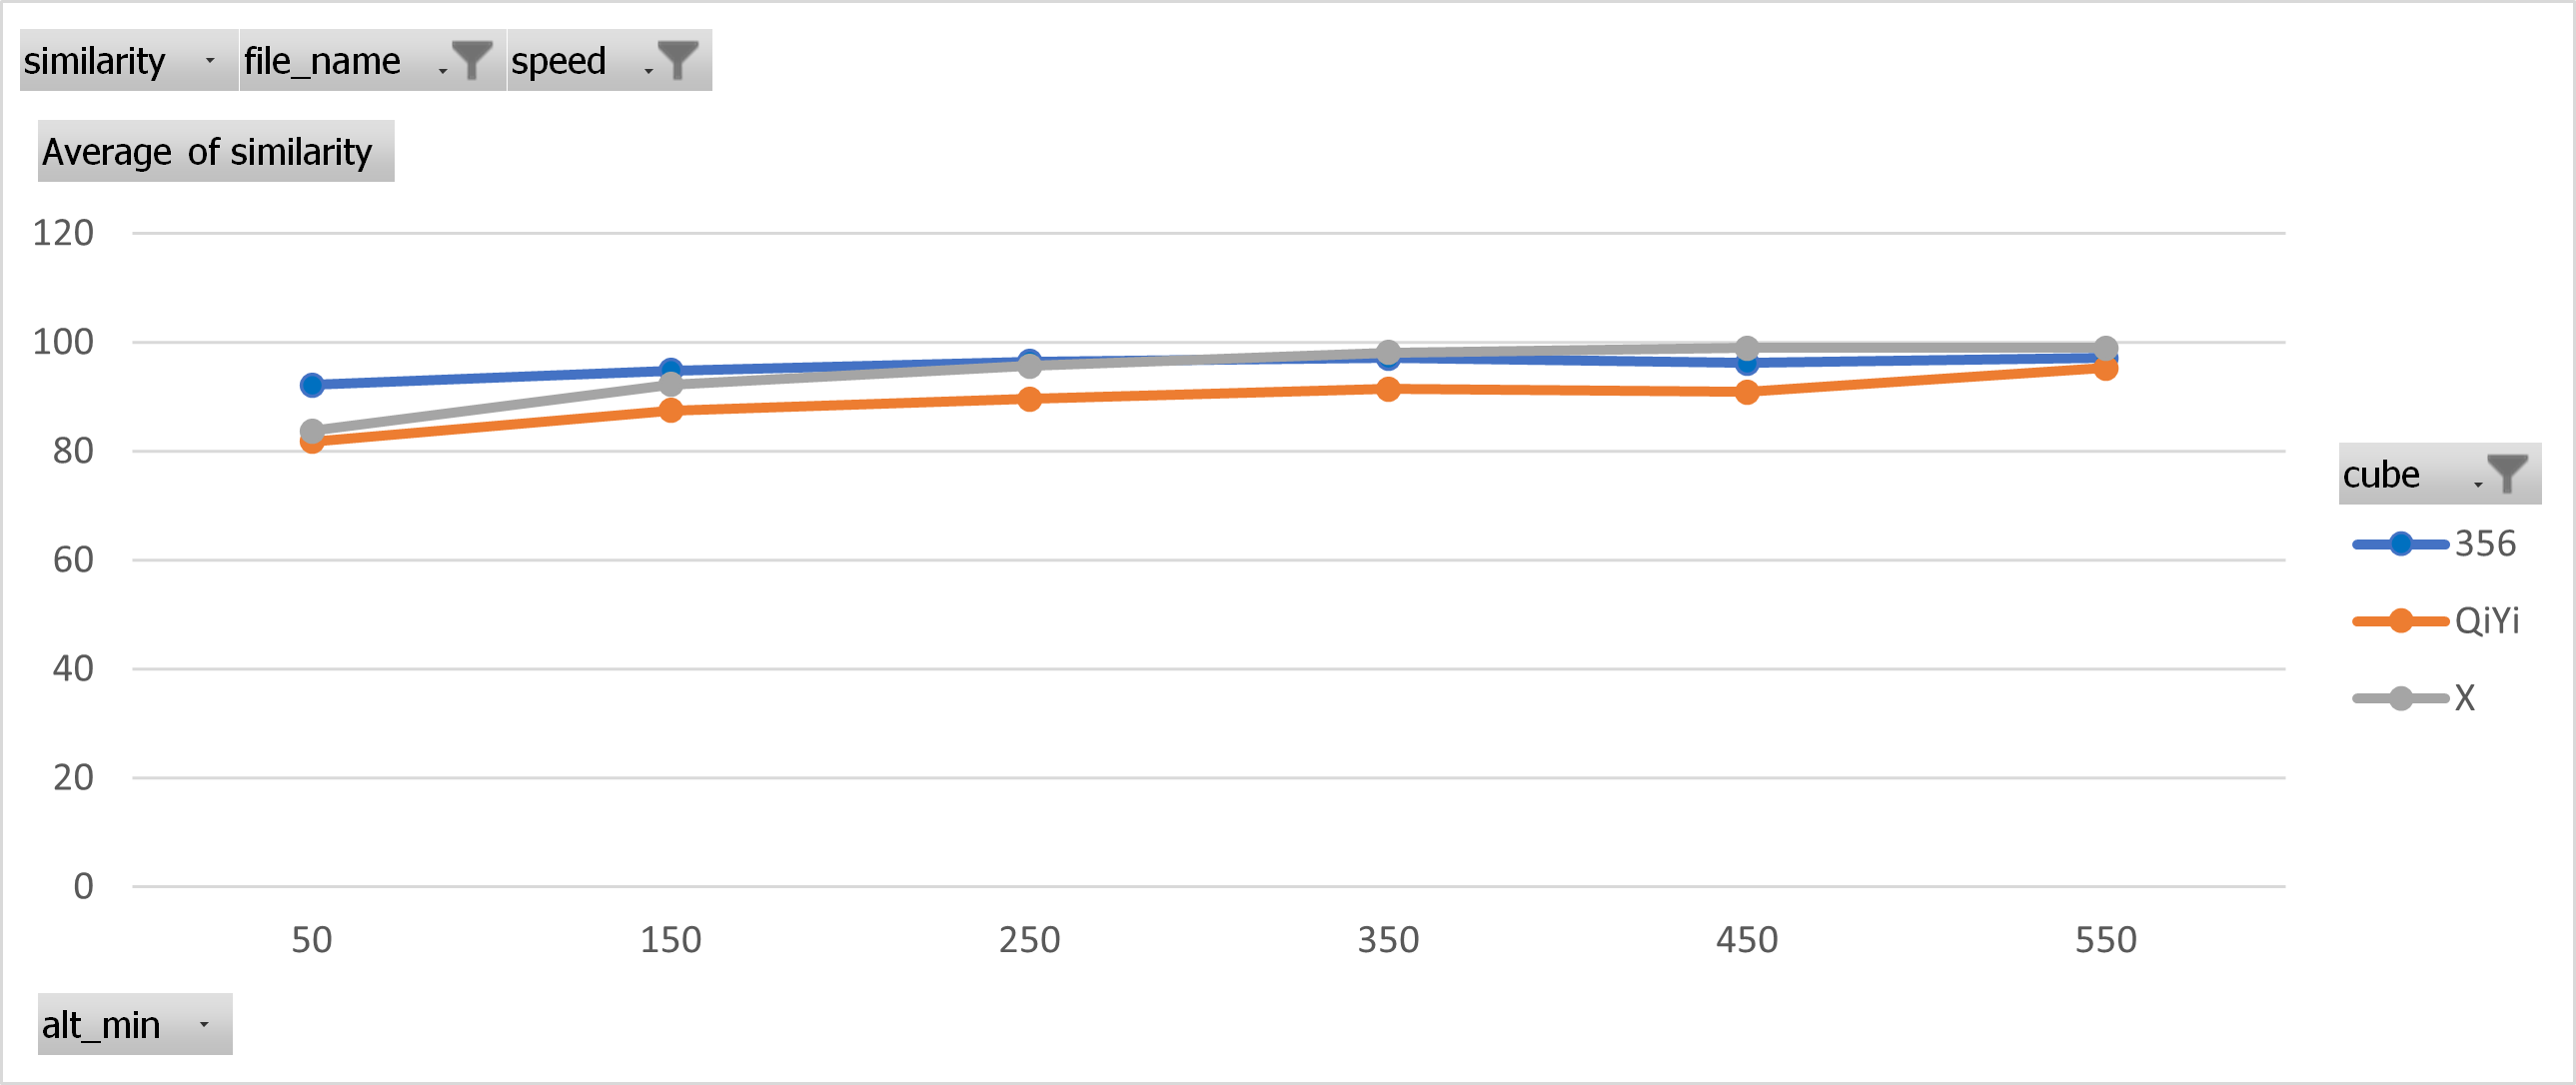
\includegraphics[width=\linewidth]{Figures/7 Evaluation/similarity_by_alt_min_2tps.png}
        \vspace*{.1mm}
    \end{subfigure}\\
    \begin{subfigure}{\textwidth}
        \centering
        \caption{Average Accuracy by Minimum Threshold at 5 TPS}
        \label{fig:influence-alt-min-average-5tps}
        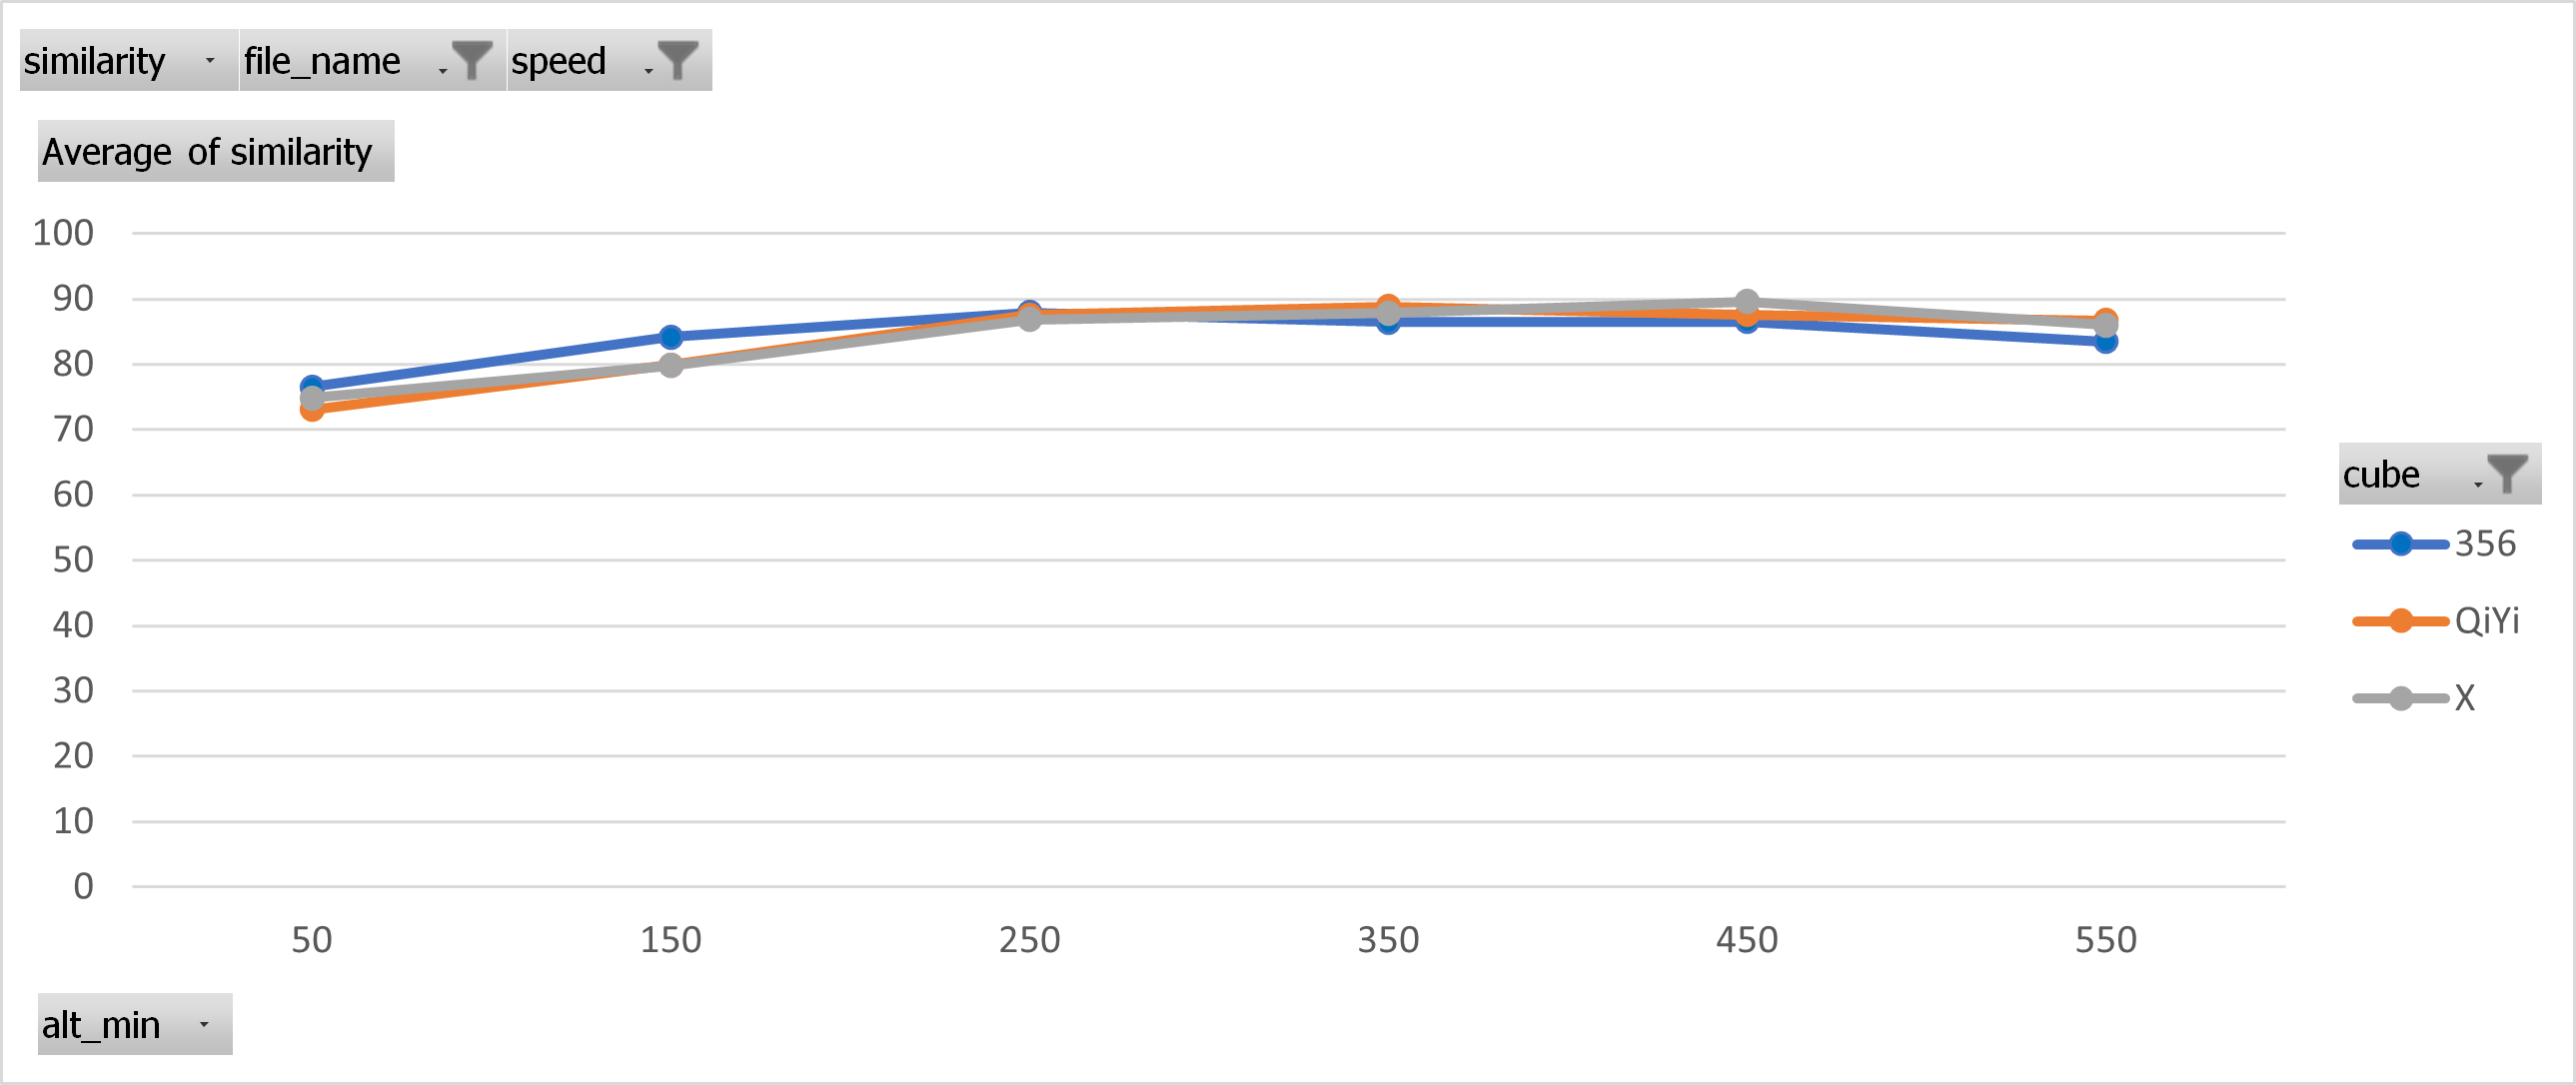
\includegraphics[width=\linewidth]{Figures/7 Evaluation/similarity_by_alt_min_5tps.png}
        \vspace*{.1mm}
    \end{subfigure}\\
\end{figure}


\subsection{Influence of Window Size}
\label{subsec:influence-window-size}

The final parameter tested in this experiment was the size of the
sliding window used to ensure that detected face turns had stabilized
before accepting them as real face turns. Since erroneous detections
rarely last for more than a few time steps, a higher window size was
expected to correspond to a higher detection accuracy.

Figure \ref{fig:influence-window-size} clearly shows that a window size
of five to ten time steps was consistently correlated with a higher
accuracy of detection. In fact, at 2 TPS, a window size of five to ten
corresponded to a nearly perfect \emph{average} detection for all
cubes, across the wide variation in the threshold parameters.

Furthermore, Figure \ref{fig:influence-window-size-average-5tps} shows
that a window size between five and eight time steps corresponded to
>90\% detection accuracy across all variations in the threshold
parameters, three to ten percentage points higher than the best
averages achieved by either threshold parameter.

\begin{figure}
    \caption{Perfect Detections by Window Size}
    \label{fig:influence-window-size}
    \begin{subfigure}{\textwidth}
        \centering
        \caption{Total number of perfect detections}
        \label{fig:perfect-detections-by-window-size-total}
        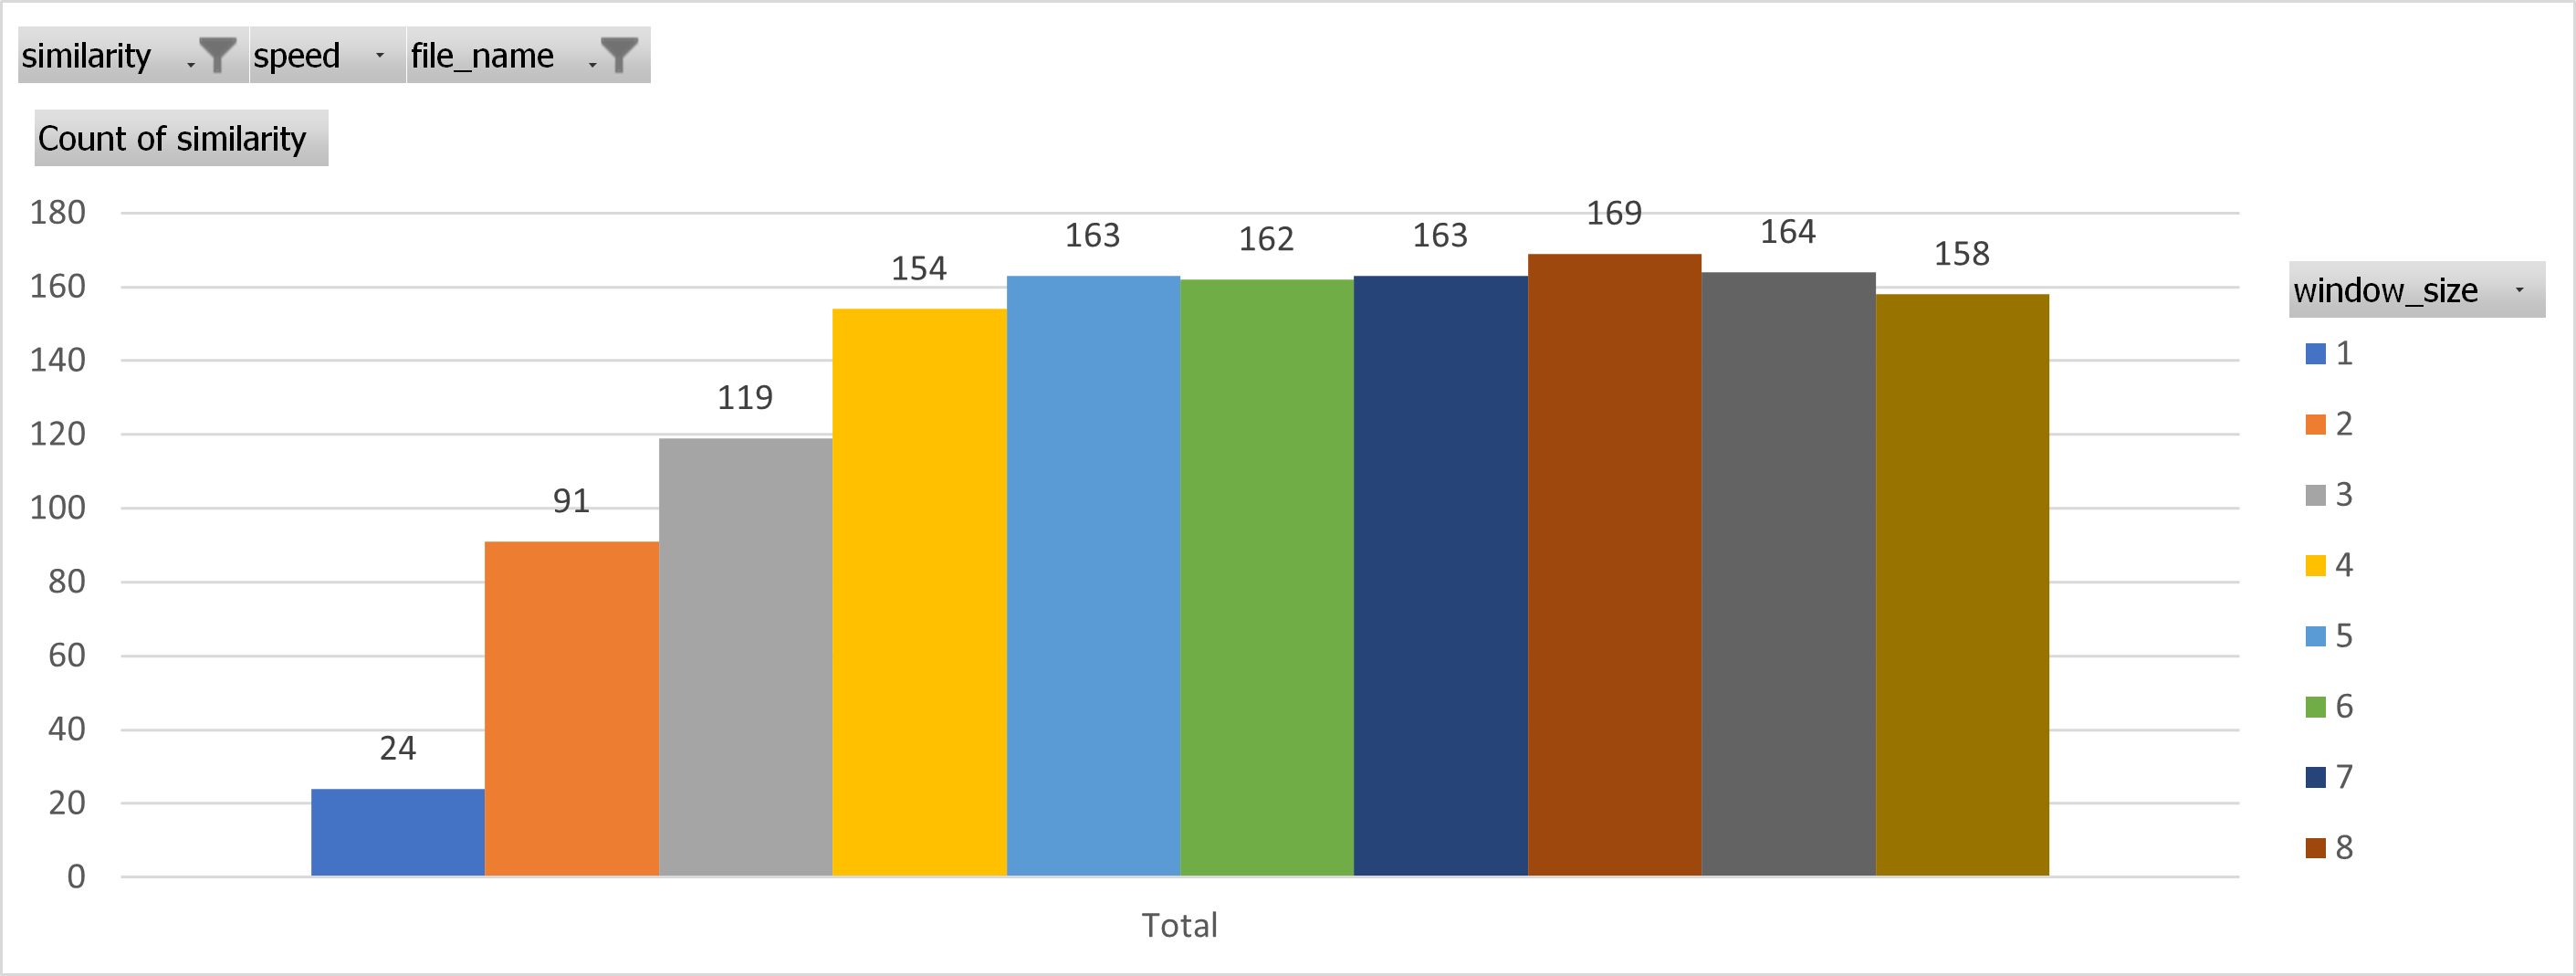
\includegraphics[width=\linewidth]{Figures/7 Evaluation/perfect_detections_by_window_size.png}
        \vspace*{.1mm}
    \end{subfigure}\\
    \begin{subfigure}{\textwidth}
        \centering
        \caption{Average Accuracy by Window Size at 2 TPS}
        \label{fig:influence-window-size-average-2tps}
        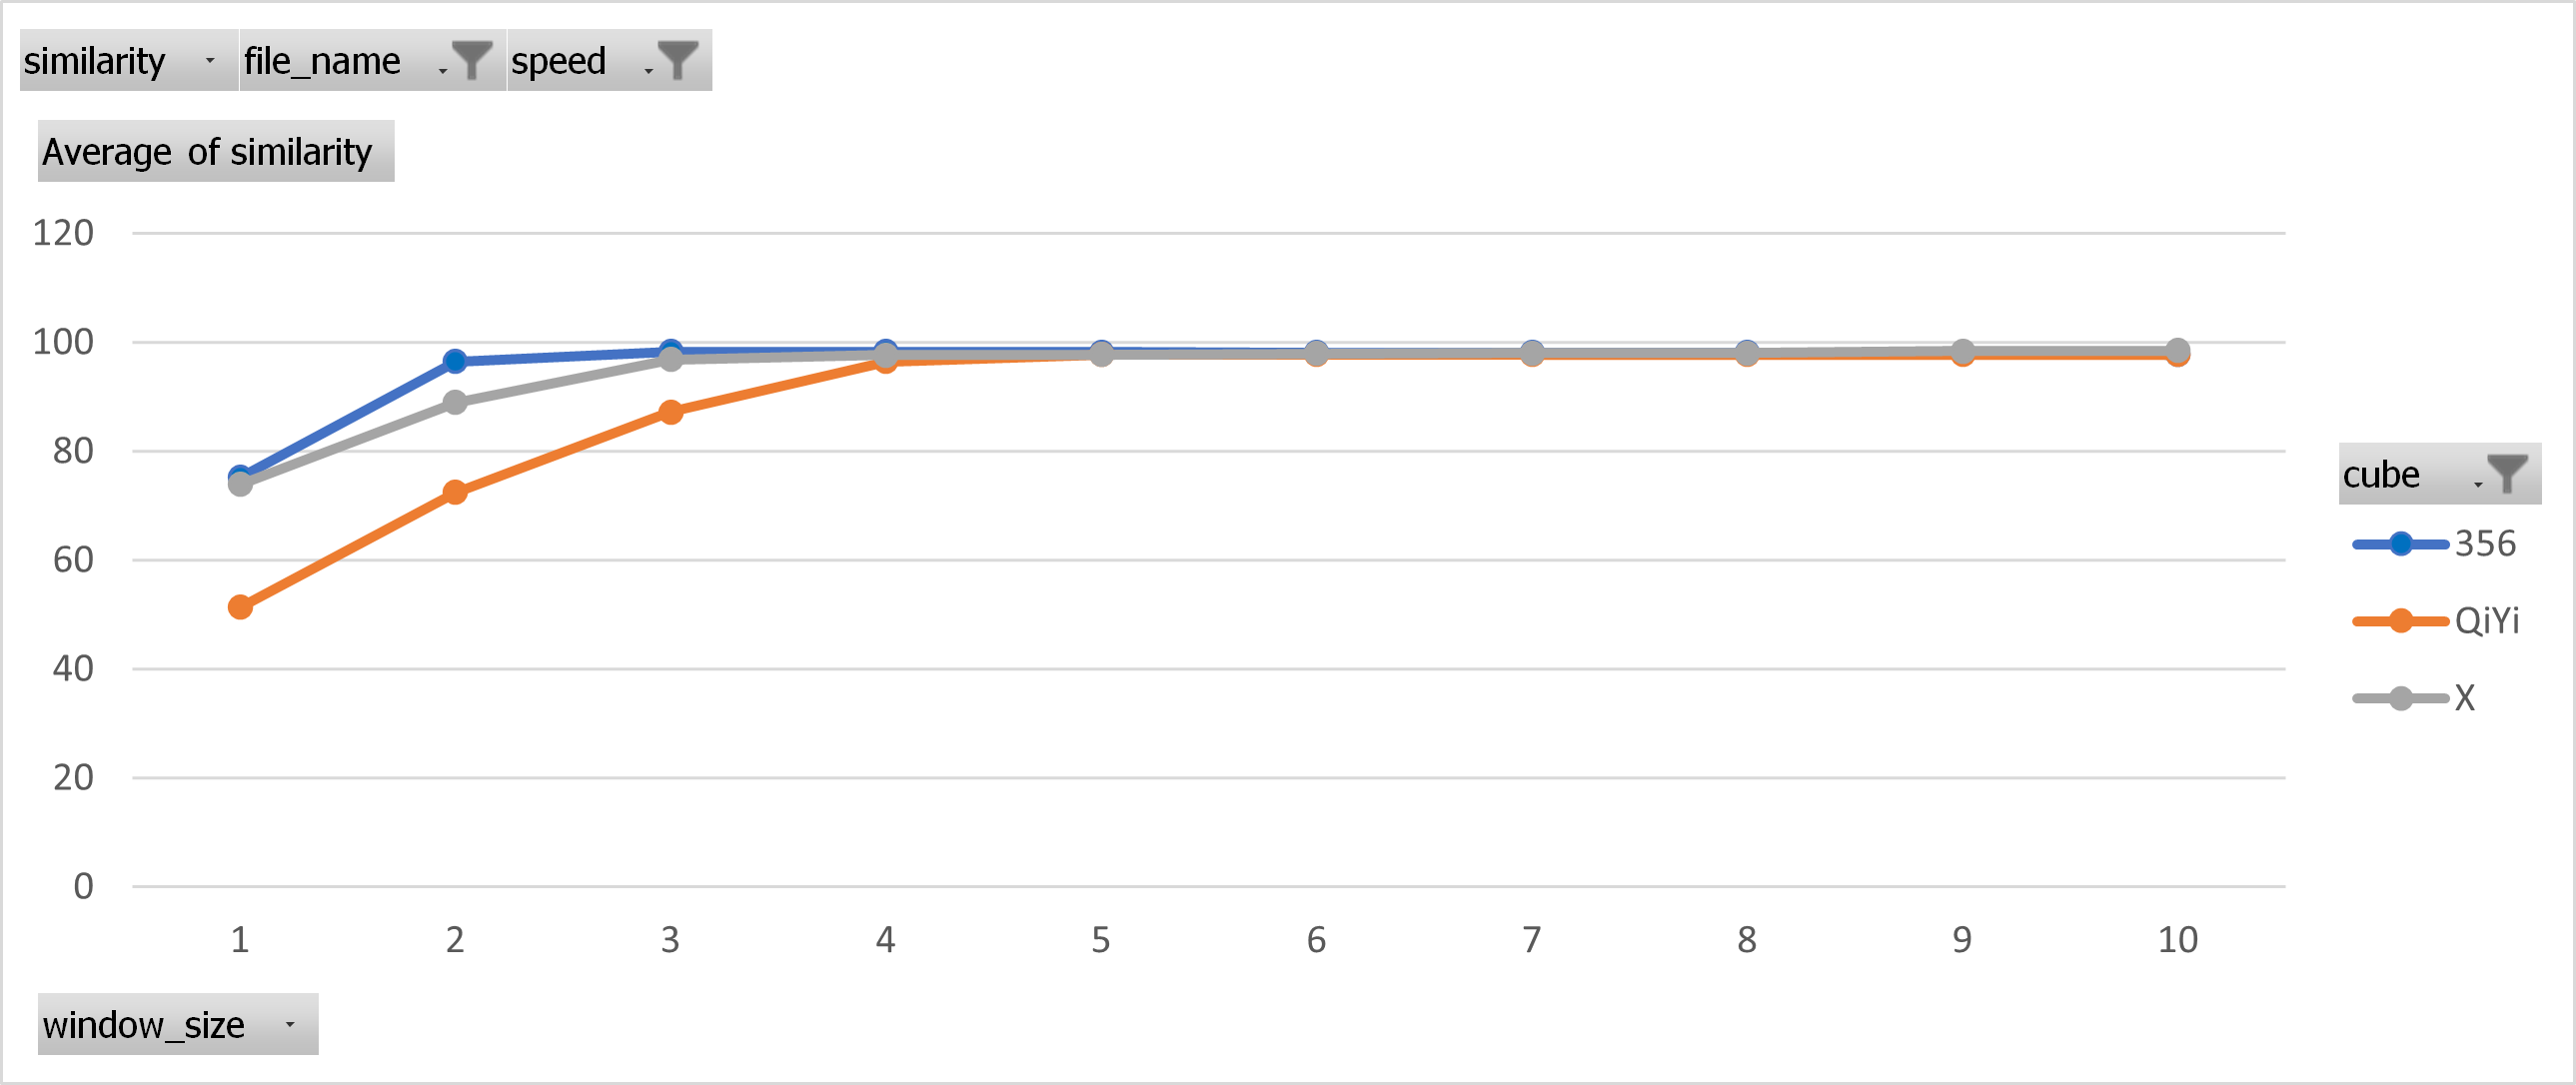
\includegraphics[width=\linewidth]{Figures/7 Evaluation/similarity_by_window_size_2tps.png}
        \vspace*{.1mm}
    \end{subfigure}\\
    \begin{subfigure}{\textwidth}
        \centering
        \caption{Average Accuracy by Window Size at 5 TPS}
        \label{fig:influence-window-size-average-5tps}
        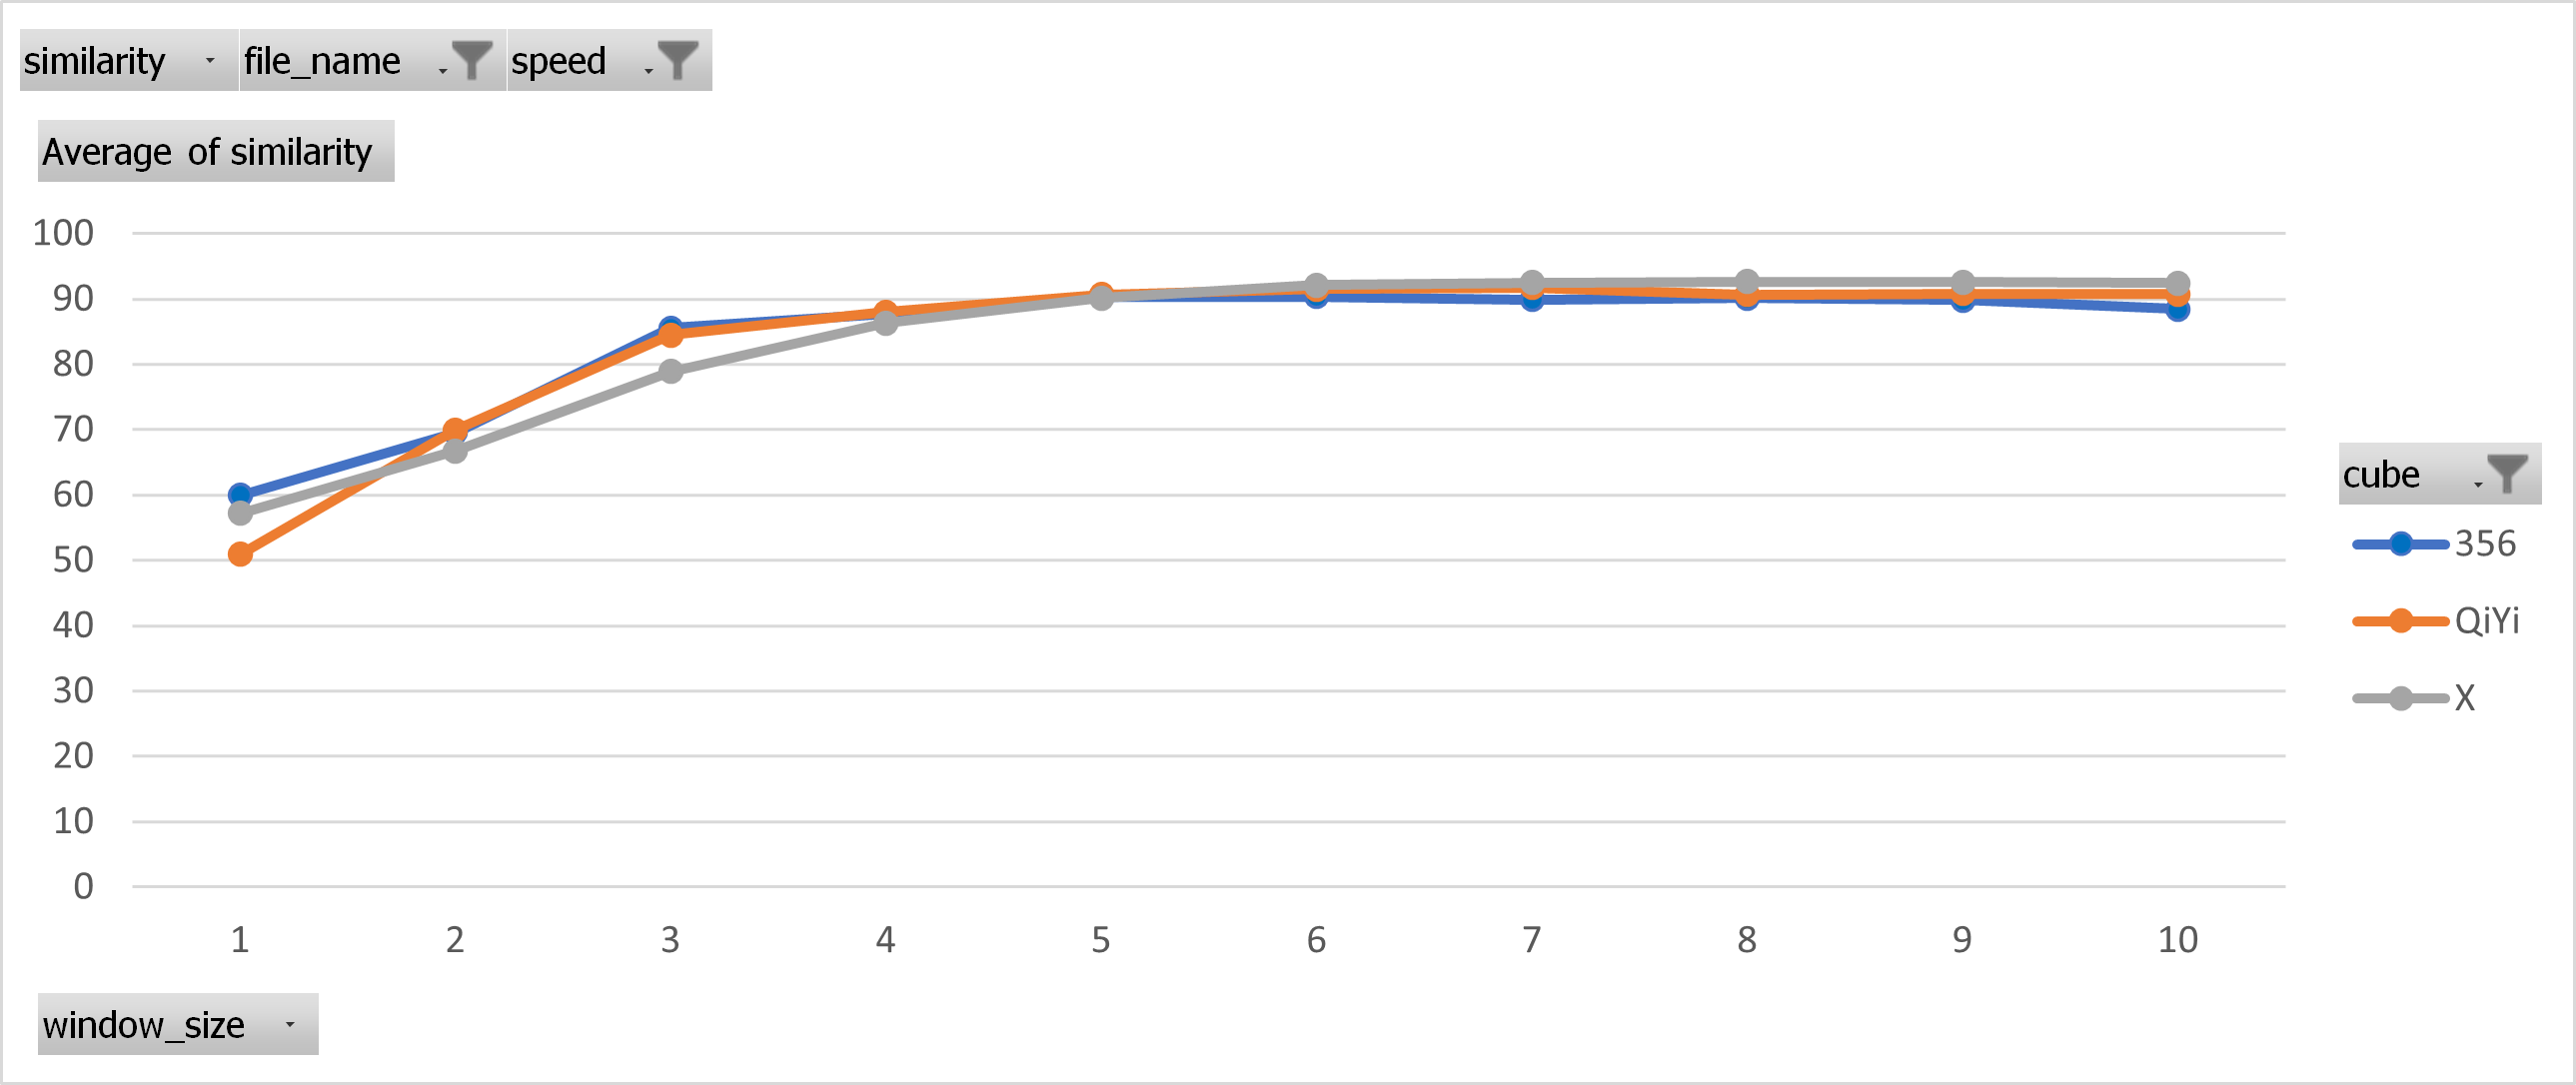
\includegraphics[width=\linewidth]{Figures/7 Evaluation/similarity_by_window_size_5tps.png}
        \vspace*{.1mm}
    \end{subfigure}\\
\end{figure}


\section{Compatibility with Standard Speedcubes}
\label{sec:compatibility-with-standard-speedcubes}

Since a major goal of this research project is to allow speedcubers to
practice with the same cube they compete with, it is imperative that
the proposed design function without requiring permanent modifications
to the original speedcube. For the same reason, the design must also
retain the original performance of the speedcube as much as possible.

As shown in Figure \ref{fig:core-placement}, the proposed PCB
transmitter can be deployed in a Gans 356 speedcube by simply changing
out the original centercap for a custom-built one containing the
transmitter. The modifications to the cube are purely temporary since
the original cube can be perfectly restored by simply replacing the
original centercaps.

The performance impact of the custom centercaps with the transmitters
is also small since the little weight they add to the cube is placed
close to the axes of rotation. On the Gans 356, a stock centercap has a
mass of 0.6719 grams, while the custom centercap shown in Figure
\ref{sec:miniaturization} has a mass of 1.6905 grams. Multiplying the
approximately 1.2 gram difference per centercap by the six centercaps
on the cube results in a 7.2 gram increase in mass for the entire
speedcube for a total mass of 91.3104 grams. Since the stock Gans 356
has a mass of 84.1204 grams, this is only an 8.6\% increase in mass,
which is within the range of variation between different
speedcubes.\footnote{For example, the acclaimed MoYu WeiLong GTS3 M has
a mass of 92g \cite{moyu-thecubicle}. More information about the
variation in masses of different speedcubes can be found at
\href{https://www.thecubicle.com/collections/3x3-speed-cubes}{TheCubicle.com}.}
This additional weight does increase the moment of interia of each
face; however, this increase is small because the added weight placed
close to the axes of rotation. As such, the corresponding performance
penalty of the extra weight would be small.


\section{Move Tracking Granularity}
\label{sec:move-tracking-granularity}

While tracking the moves performed on the speedcube constitutes the
minimum viable functionality for a design, additional features make a
design a more useful solution to the speedcubing community. Of most
value is the ability to track the amount of time spent performing each
face turn; from that single metric many other highly valuable metrics
can be derived like TPS over time, and time spent completing each stage
of the solution.

Though not shown in the pretty printed algorithm from Section
\ref{subsec:ignoring-noise-when-extracting-move-sequences}, the
proposed software receiver also records the time stamp at which it
detected each face turn. By computing the difference between time
stamps, one can calculate the amount of time spent performing each
individual face turn. While not implemented in this design, a more
sophisticated software receiver could provide even more precise
measurements from the same source data by measuring the amount of time
between stable signals for each centerpiece state.

However, since this design does not include a gyroscope, it cannot
provide metrics about cube orientation over time like the highest-end
commercial smartcubes. As such, this design cannot be used to directly
report x, y, and z cube rotations, those sophisticated post-processing
heuristics could predict their locations with decent accuracy.


\section{Competition Legality}
\label{sec:competition-legality}

As discussed in Section \ref{subsec:competition-regulations},
speedsolving competitors cannot use any electronics or audio equipment
while solving the cube in competition. Since a major goal of this
research project is to allow speedcubers to practice with the same cube
they compete with, a design must either inherently comply with existing
competition rules against the use of electronics or must result in a
cube that can be easily modified to regain compliance.

While the design proposed in this thesis, certainly does not inherently
comply with the existing competition regulations since it requires
embedding electronics into the cube, it does result in a cube that can
be easily modified to regain compliance. As mentioned in Section
\ref{sec:compatibility-with-standard-speedcubes}, the only modification
to the cube is an interchangeable centercap that can be easily removed
and replaced with the original centercap to produce a perfectly
competition-legal cube.

Interestingly, the sound-based nature of this design provides a
potential compromise on the use of smart cubes in competition. As
mentioned at the end of Section \ref{sec:minimizing-sound-obstruction},
a sound-based transmitter only works at a short range and can easily be
rendered inaccessible to a competitor by scrambling cubes several
meters away from the competitors (especially in a different room), or
playing audio at the same frequencies as the transmitter. As such,
these properties of sound-based turn tracking could provide an avenue
in which smart cubes could be safely allowed in competitions to aid in
solve reconstructions without enabling competitors to spy on scrambles.

\section{Summary}

In summary, this chapter explored the effectiveness of the design
proposed in Chapters \ref{Chapter4}, \ref{Chapter5}, and \ref{Chapter6}
against four benchmarks derived from the research questions outlined in
Section \ref{sec:research-questions}.

The analysis of the receiver algorithm revealed many configurations
that enabled it to achieve a perfect detection accuracy. Most impactful
in that detection was the usage of a high \code{window\_size} which
achieved accuracies of over 90\% across all variations in the other
parameters. Additionally beneficial is the receiver's ability to detect
the time between face turns which opens the door to calculating useful
metrics like TPS over time.

The analysis of the transmitter also found promising results. A rough
prototype of the PCB was small enough to fit into a single centercap
without requiring any permanent modifications to the cube. Furthermore,
since the centercap was interchangeable, the electronic components
impermissible in competition could easily be removed to return the cube
to a competition-legal state. In addition, the added mass of the
electrical components did not significantly increase the weight of the
puzzle, nearly retaining its original performance.
 
% Chapter Template

\chapter{Conclusion} % Main chapter title

\label{Chapter8} % Change X to a consecutive number; for referencing this chapter elsewhere, use \ref{ChapterX}


\section{Summary}

TODO summarize the goals from the Introduction and broadly describe
what techniques were most helpful in reaching them. Also detail a
summary of exactly how effective they were.

\section{Answering Research Questions}
\label{sec:answering-research-questions}

Chapter \ref{Chapter3} concluded with a detailed list of research
questions that would be explored in this thesis (see Section
\ref{sec:research-questions}). This section provides direct, summarized
answers to each of those questions.

Section \ref{subsec:answer-feasibility} summarizes the constraints for
a sound-based move tracking protocol. Section
\ref{subsec:answer-accuracy} then reports on the accuracy achieved by
the proof-of-concept proposed earlier in the thesis. Section
\ref{subsec:answer-compatibility} continues by reviewing the challenges
associated with building a transmitter small enough to
non-destructively embed into an existing speedcube. From there, Section
\ref{subsec:answer-granularity} discusses additional data points that
can be inferred from the transmitted audio. Finally, Section
\ref{subsec:answer-competition-legality} addresses the ways in which a
sound-based smartcube design can comply with competition regulations
banning the usage of electronics.

\subsection{Feasibility on Consumer Hardware}
\label{subsec:answer-feasibility}

\emph{What are the constraints for a sound-based smart cube design
compatible with consumer-grade microphones like those found in common
smartphones and laptops?}

As discussed in Chapter \ref{Chapter4}, there are four main factors
that affect the viability of a sound-based smart cube design: 

\begin{enumerate}
    \item the achievable \textbf{signal-to-noise ratio} of the transmitter
    \item the \textbf{distinctiveness of the tones} used for the protocol
    \item the \textbf{frequency response range of consumer hardware} used to implement the protocol
    \item the \textbf{range of tones audible} to the human ear
\end{enumerate}

An analysis of these factors found that the tones used in the protocol
should be (1) broadcast with an audio intensity of -30dB or greater
(see Section \ref{subsec:signal-to-noise-ratio}) and (2) spaced at
least 100Hz apart (see Section \ref{subsec:tone-distinctiveness}) in
order to have a sufficiently strong signal-to-noise ratio for clear
detection. Furthermore, the specific tones chosen for the protocol
would ideally fit within the "musical range" of 500Hz and 4000Hz to
simultaneously (4) avoid irritating human solvers (see Section
\ref{subsec:human-auditory-range}) and (3) leverage the optimizations
built into consumer audio recording hardware in smartphones and laptops
(see Section \ref{subsec:frequency-response-range}).

\subsection{Move Tracking Accuracy}
\label{subsec:answer-accuracy}

\emph{How could a sound-based smart cube design track the face turns of
a Rubik's Cube with high accuracy?}

As discussed in Section \ref{sec:move-tracking-accuracy}, the receiver
from Chapter \ref{Chapter5} and the transmitter from Chapter
\ref{Chapter6} were able to transmit and decode a sequence of face
turns with perfect accuracy across a variety of input parameters within
a controlled environment. \footnote{Specifically, this controlled
environment consisted of synthetically generated audio representative
of the output of an ideal transmitter (see Sections
\ref{sec:synthetic-audio-generation} and
\ref{sec:adding-realistic-noise}) played from a Google Pixel phone and
recorded by an HP Spectre laptop in a quiet room (see Section
\ref{subsec:signal-to-noise-ratio}).}

Various factors aided in these results. First, each face position is
associated with a signal present in a unique frequency band (See
Section \ref{subsec:tone-distinctiveness}). This separation of
frequencies makes it easier to distinguish changes in the state of
independent faces on the cube. Second, the current position of each
face is continuously broadcast, increasing the amount of time available
for the receiver to detect and decode each position over time (See
Section \ref{sec:alternatives}). Third, multiple layers of noise
filters were applied within the receiver to better focus on the true
signal frequencies and boost confidence in the accuracy of the decoded
face turns (See Section \ref{sec:decoding-realistic-noise}).


\subsection{Compatibility with Standard Speedcubes}
\label{subsec:answer-compatibility}

\emph{How could a sound-based smart cube design be deployed within a
standard, "non-smart" speedcube without requiring permanent
modifications to the original cube?}

The key challenges involved in creating a sound-based smartcube
enhancement for an existing speedcube stem from the size constraints
imposed by the structure of the cube. Since all modifications must be
non-destructive, the required electronics must be embedded into the
empty spaces within the cubies on the cube. Furthermore, since neither
the edges nor the corners on the cube have access to the axles on which
the cube rotates, the best place for these electronics is within the
centercaps themselves. Unfortunately, these centercaps offer little
space for add-ins. For example, as discussed in Sections
\ref{subsec:prospects-of-miniaturization} and
\ref{sec:miniaturization}, the relatively spacious Gans 356 only offers
space for a $16mm^2$ PCB with rounded corners and a $6mm$ diameter hole
in the middle.

Despite these stringent size constraints, Chapter \ref{Chapter6}
specifies a promising transmitter design consisting of less than 10
discrete electrical components. With this limited component count, a
PCB consisting of SMD components would be able to fit within a
custom-printed centercap for a Gans 356 speedcube as shown in Figure
\ref{fig:core-placement}.\footnote{Note that an actual PCB was not
constructed nor was a PCB layout attempted for any other cube than the
Gans 356.}

As discussed in Section
\ref{sec:compatibility-with-standard-speedcubes}, since the required
electronics are contained within a replaceable, custom centercap, the
modifications can be easily reversed by replacing the custom centercaps
with the originals.


\subsection{Move Tracking Granularity}
\label{subsec:answer-granularity}

\emph{How could a sound-based smart cube design record the time spent
executing each individual face turn of a Rubik's Cube?}

The receiver proposed in Chapter \ref{Chapter5} decodes face turns by
iterating over a time series of audio data. As a result, when a face
turn is detected, the receiver also knows the time at which it
occurred. By computing the difference between the times at which two
successive turns occurred, the time spent executing an individual face
turn can be computed. Thus, as long as the receiver can detect the face
turns applied to the cube with high accuracy, then the time spent
executing each one can be easily calculated (See also Section
\ref{sec:move-tracking-granularity}).


\subsection{Competition Legality}
\label{subsec:answer-competition-legality}

\emph{How could a sound-based smartcube design comply with competition
regulations prohibiting the use of electronics while performing a
competitive solve?}

Since the use of electronics while competitively solving a Rubik's Cube
is banned by WCA regulation 2i \cite{wca-regulations}, any move
tracking solutions must not permanently embed electronics into the
structure of the cube.

The solution proposed in Section
\ref{subsec:prospects-of-miniaturization} is to create a tiny sound
transmitter that can be embedded into a custom centercap. Such a
transmitter can be temporarily installed during personal practice then
replaced with the original centercaps during competitions.

Alternatively, since the signal of a sound-based transmitter can be
blocked by by a physical wall or purposefully broadcasting interfering
signals in the same frequency range, it's possible that, with proper
negotiation with the WCA, a sound based move tracking solution could be
deemed competition legal.


\section{Limitations}
\label{sec:limitations}

As stated in Section \ref{sec:research-questions}, the overarching goal
of this thesis is to present a proof-of-concept for a sound-based smart
cube design. Like all proofs-of-concept, the design proposed in this
thesis contains some inherent flaws and underlying assumptions that limit
its ability to be successfully deployed in existing speedcubes.

First, while Chapter \ref{Chapter6} demonstrates that its proposed
transmitter design appropriately considers all relevant requirements, a
fully functional transmitter was never built and deployed within an
existing speedcube. As such, the viability of this transmitter design
cannot be fully verified until a transmitter is fully constructed,
deployed, and tested.

Second, while great care was taken to extensively test the receiver,
all tests were conducted with realistic, but synthetic audio samples
since a physical transmitter was never built (See Section
\ref{sec:adding-realistic-noise}). As such, it is possible that further
refinements to the receiver will be required if the signals from a real
transmitter substantially differ from those synthesized for testing the
receiver.

Third, though not a functional limitation, since the typical frequency
response range of consumer hardware is entirely within the human
auditory range (see Sections \ref{subsec:frequency-response-range} and
\ref{subsec:human-auditory-range}), all frequencies selected for
transmitting the state of the cube will be human-audible. If the chosen
frequencies are higher in pitch (as recommended by Section
\ref{subsec:freq-selection}), the sounds produced by the transmitter
may prove irritating to the speedcuber. 

Fourth and finally, while the tests of the receiver achieved perfect
accuracy on all test cases (see Section \ref{subsec:answer-accuracy}),
the specific parameters used to achieve perfect accuracy differed
between each one. Since there is not one set of parameters that worked
for all test cases, additional experimentation and refinement will be
necessary to determine the best parameters for decoding face turns in
any given cube/environment combination.


\section{Outlook}
\label{sec:outlook}
TODO If I had more time/resources to work on it, what would I do next
with this project?

- Live algorithm
- build it small enough to fit in the cube.
- supersonic frequencies.

%----------------------------------------------------------------------------------------
%	THESIS CONTENT - APPENDICES
%----------------------------------------------------------------------------------------

\appendix % Cue to tell LaTeX that the following "chapters" are Appendices

% Include the appendices of the thesis as separate files from the Appendices folder
% Uncomment the lines as you write the Appendices

% Appendix A

\chapter{Longer Code Snippets} % Main appendix title
\label{appendix:code} % For referencing this appendix elsewhere, use \ref{AppendixA}

\section{Spectrogram Generation from Section \ref{subsec:decode-component-frequencies}}
This code snippet actually generates a full animation of how the component frequencies change over time. Figure \ref{fig:spectrogram} is only one frame of this animation.
\begin{verbatim}
# Heavily aided by https://matplotlib.org/stable/gallery/animation/simple_anim.html
import matplotlib.pyplot as plt
import matplotlib.animation as animation
import numpy as np
from scipy import signal
from scipy.io import wavfile

def animate(wav_path: str, alg: str):
    # Parse the audio sample into its spectrogram
    SAMPLES_PER_WINDOW = 1024  # Seems balance frequency precision with time precision.
    sample_rate, audio_samples = wavfile.read(wav_path)
    freq, time, Zxx = signal.stft(audio_samples, fs=sample_rate,
        nperseg=SAMPLES_PER_WINDOW, noverlap=(SAMPLES_PER_WINDOW // 4) * 3)
    spectrogram = np.abs(Zxx).transpose()

    # Generate the plots
    fig, (ax_spectrogram, ax_fourier) = plt.subplots(2)

    # Set the spectrogram
    ax_spectrogram.specgram(audio_samples,
        Fs=sample_rate, 
        NFFT=SAMPLES_PER_WINDOW, 
        noverlap=SAMPLES_PER_WINDOW // 4 * 3)  # 3/4 of the window size
    line_spectrogram, = ax_spectrogram.plot([], [], '-', color='red')
    time_tracker_spectrogram = ax_spectrogram.axvline(0, color='red')
    ax_spectrogram.set_ylim(0, 4000)
    ax_spectrogram.set_title(f"Spectrogram")
    ax_spectrogram.set_ylabel('Frequency [Hz]')
    ax_spectrogram.set_xlabel('Time [sec]')

    # Set the Fourier transform
    STEP = 10
    indices = np.arange(0, len(time) + 1, step=STEP)
    line_fourier, = ax_fourier.plot(freq, spectrogram[0], color='red')
    ax_fourier.set_title("")
    ax_fourier.set_xlim(0, 4000)  # Frequency
    ax_fourier.set_xlabel("Frequency [Hz]")
    ax_fourier.set_ylim(0, np.amax(spectrogram))  # Strength
    ax_fourier.set_ylabel("Strength")

    # Space figures nicely
    fig.suptitle(alg)
    fig.tight_layout(h_pad=3)

    def draw_frame_at(i):
        time_tracker_spectrogram.set_xdata(time[i])
        line_fourier.set_ydata(spectrogram[i])
        ax_fourier.set_title(f"Frequencies at {time[i]:.2f} seconds")
        return line_spectrogram, line_fourier

    ani = animation.FuncAnimation(fig, draw_frame_at,
        frames=indices, interval=1, blit=True, save_count=len(time)/STEP)
    ani.save(f"plt/animation/{wav_path[:-4]}.mp4",
        fps=len(time)/STEP/5, dpi=300)
    plt.show()

animate(demo_wav_path, demo_alg)
\end{verbatim}


%\include{Appendices/AppendixB}
%\include{Appendices/AppendixC}

%----------------------------------------------------------------------------------------
%	BIBLIOGRAPHY
%----------------------------------------------------------------------------------------

\printbibliography[heading=bibintoc]

%----------------------------------------------------------------------------------------

\end{document}  
